\documentclass[10pt,a4paper,twoside,openright]{book}

\input{../../../Libri/template_dispense.tex}

	\usepackage{geometry}
	\geometry{
		nomarginpar, % Toglie doppi margini
		margin=1in, % Imposta i margini a 1 inch
	}

%\usepackage{chngcntr}
%\counterwithout{figure}{chapter}
%\counterwithout{equation}{chapter}

\allowdisplaybreaks[4] % Consente di rompere equazioni su più pagine

%%%%%%%%%%%%%%%%%%%%%%%%%%%%%%%%%%%%%%%%%%%%%%%
%%%%%%%%%%%%%%%%%%%%%%%%%%%%%%%%%%%%%%%%%%%%%%%


\begin{document}


%%%%%%%%%%%%%%%%%%%%%%%%%%%%%%%%%%%%%%%%%%%%%%%
%%%%%%%%%%%%%%%%%%%%%%%%%%%%%%%%%%%%%%%%%%%%%%%

\frontmatter
\pagestyle{empty} % SWITCHA PER NON AVERE NUMERO PAGINA
\vspace*{\fill}
%Teo Bucci \\
\begin{center}
	{\large \textsc{Appunti di}}\\
	\vspace*{0.4cm}
	{\Huge \textsc{Equazioni alle Derivate Parziali}}\\
	\vspace*{0.3cm}
	{\huge \textsc{Parte Analitica}}\\
	\vspace*{1cm}
	{\large {Dalle lezioni del Prof. Sandro Salsa \& Gianmaria Verzini}}\\
	\vspace*{0.1cm}
	{\large per il corso di Ingegneria Matematica}\\
	\vspace*{0.4cm}
	{\large {di Teo Bucci \& Filippo Cipriani}}\\
	\vspace*{1cm}
	Politecnico di Milano\\A.A. 2020/2021
\end{center}
\vspace*{\fill}
\newpage

%%%%%%%%%%%%%%%%%%%%%%%%%%%%%%%%%%%%%%%%%%%%%%%
%%%%%%%%%%%%%%%%%%%%%%%%%%%%%%%%%%%%%%%%%%%%%%%

{\Large \textit{Appunti di Equazioni alle Derivate Parziali}}

\vspace*{\fill}

\textcopyright \ Gli autori, tutti i diritti riservati

Sono proibite tutte le riproduzioni senza autorizzazione scritta degli autori.

Revisione del \today

Developed by\\
Teo Bucci - \texttt{teobucci8@gmail.com}\\
Filippo Cipriani - \texttt{filippcipriani@gmail.com}\\ \\
Compiled with \ensuremath\heartsuit \\

%\textbf{Prefazione}

Per segnalare eventuali errori o suggerimenti potete contattare gli autori.

\newpage

%%%%%%%%%%%%%%%%%%%%%%%%%%%%%%%%%%%%%%%%%%%%%%%
%%%%%%%%%%%%%%%%%%%%%%%%%%%%%%%%%%%%%%%%%%%%%%%

% INDICE
\addtocontents{toc}{\protect\thispagestyle{empty}}
\tableofcontents
%\newpage

%%%%%%%%%%%%%%%%%%%%%%%%%%%%%%%%%%%%%%%%%%%%%%%
%%%%%%%%%%%%%%%%%%%%%%%%%%%%%%%%%%%%%%%%%%%%%%%

% PAGINA VUOTA PER FAR PARTIRE IL CAPITOLO IN UNA PAGINA DISPARI
%\myNewEmptyPage

\AtEndDocument{\cleardoublepage}

%%%%%%%%%%%%%%%%%%%%%%%%%%%%%%%%%%%%%%%%%%%%%%%
%%%%%%%%%%%%%%%%%%%%%%%%%%%%%%%%%%%%%%%%%%%%%%%

\mainmatter
\pagestyle{fancy} % RISWITCHA PER RIAVERE IL NUMERO PAGINA
%\setcounter{page}{1} % FA RIPARTIRE IL CONTATORE PAGINA DA 1

%%%%%%%%%%%%%%%%%%%%%%%%%%%%%%%%%%%%%%%%%%%%%%%
%%%%%%%%%%%%%%%%%%%%%%%%%%%%%%%%%%%%%%%%%%%%%%%


















































































































































































































































































































































\part{Equazioni alle Derivate Parziali}
\chapter{Modelli matematici}

Un modello matematico è un compromesso tra complessità del mondo reale e idee astratte della matematica. Li applicheremo spesso nel contesto della meccanica dei continui.

Ci serviranno due mattoni principali
\begin{itemize}
\item leggi generali (conservazione, bilancio dell'energia, della massa, della carica
\item leggi costitutive, di natura sperimentale, costruite ad hoc per catturare la natura essenziale del fenomeno che osserviamo (di Fourier, di Fiek, di Ohm...)
\end{itemize}

Si perviene quindi a equazioni o sistemi di equazioni ordinarie o alle derivate parziali.

Una EDP è un'equazione della forma
\begin{equation*}
F( x,t,u,u_{t},u_{x_{j}},u_{x_{i} x_{j}},\dotsc)
\end{equation*}
L'ordine di un'equazione è l'ordine massimo di derivazione.
\section{Distinzione di EDP}

Si distinguono
\begin{itemize}
\item equazioni lineari: $F$ è un polinomio di primo grado in $u$ e in tutte le derivate parziali
\item equazioni non lineari
\begin{itemize}
\item semilineari: $F$ è non lineare solo rispetto ad $u$
\item quasilineari: $F$ è lineare nelle derivate di ordine massimo, con coefficiente che possono dipendere da $u$ e dalle derivate di ordine inferiore
\item completamente non lineari: $F$ è non lineare nelle derivate di ordine massimo
\end{itemize}
\end{itemize}
\begin{definition}
[Laplaciano] Definiamo il laplaciano di $\displaystyle u=u( x_{1},\dotsc,x_{n})$
\begin{equation*}
\Delta u=\sum ^{n}_{j=1}\frac{\partial ^{2} u}{{\partial x_{j}}^{2}}
\end{equation*}
\end{definition}
\textit{Esempi.}
\begin{itemize}
\item Lineare

\textit{Calore o diffusione}

\begin{equation*}
u_{t} -D(x,t) \Delta u=f
\end{equation*}

\textit{Laplace/Poisson}

\begin{equation*}
\Delta u=f(x,t)
\end{equation*}

\textit{Onde}

\begin{equation*}
u_{tt} -c^{2} \Delta u=0\ \ \ c(x,t)
\end{equation*}
\item Non lineare
\begin{itemize}
\item Semilineare

\textit{Fisher-Kolmogorov}\begin{equation*}
u_{t} -D\Delta u=f(u) =ru(1-u)
\end{equation*}
\item Quasi lineare

\textit{Burgers}\begin{equation*}
u_{t} +u\cdotp u_{x} =\varepsilon u_{xx} \ \ \ \ x\in \mathbb{R}
\end{equation*}

\textit{Equazione delle superfici minime (o delle bolle di sapone)}\begin{equation*}
\mathrm{div}\left(\frac{\nabla u}{\sqrt{1+| \nabla u| ^{2}}}\right) =0
\end{equation*}
\item Completamente non lineare

\textit{Iconale} (ottica geometrica)\footnote{$c(x)$ è l'indice di rifrazione.}\begin{equation*}
| \nabla u| ^{2} =c(x)
\end{equation*}

\textit{Altro esempio di equazione completamente non lineare.}

Sia $u=u(x),x\in \mathbb{R}$, consideriamo un'equazione del secondo ordine lineare\begin{equation*}
\mathcal{L} u=\sum ^{n}_{i,j=1} a_{ij}(x) u_{x_{i} x_{j}} =a_{11}(x) u_{x_{1} x_{1}} +\dotsc +a_{nn}(x) u_{x_{n} x_{n}}
\end{equation*}Prendo due operatori del tipo $\mathcal{L}_{1} u$ e $\mathcal{L}_{2} u$. Allora\begin{equation*}
F(u)(x) =\max\{\mathcal{L}_{1} u(x),\mathcal{L}_{2} u(x)\}
\end{equation*}è completamente non lineare.
\end{itemize}
\end{itemize}

Se è presente il tempo, si possono assegnare delle condizioni iniziali.
\section{Problema ben posto}

Compito dell'analisi teorica è, una volta costruito il modello consono, è stabilire quale tipo di dati è necessario assegnare per ottenere
\begin{enumerate}
\item Esistenza di una soluzione
\item Unicità
\item Dipendenza continua dai dati
\end{enumerate}

Un problema di questo tipo è un problema ben posto\footnote{secondo Hadamand.}.



L'esistenza è un controllo di consistenza, perché il modello non è la realtà, ma cerca di copiarla.
\begin{gather*}
\mathrm{div}(\nabla u) =\Delta u=0\\
\mathrm{div}(a(x) \nabla u) =\nabla a\cdotp \nabla u+a\Delta u
\end{gather*}
Voglio $u\in C^{2}$, ci sono problemi se esce un termine $a$ che tiene conto dell'anisotropia (discontinuità), perché $\nabla a$ non ha senso, essendo discontinuo.



L'unicità è importante per l'approssimazione, vogliamo essere certi che ci sia un'unica soluzione a cui far tendere l'approssimazione.



La dipendenza continua dai dati è importante perché è una forma di \textit{stabilità} rispetto all'argomento. In generale, siano $g_{1},g_{2}$ i dati di un problema e $u_{1},u_{2}$ le corrispondenti soluzioni. Vi è stabilità se
\begin{equation*}
\text{dist}(g_{1},g_{2})\rightarrow 0\ \ \Rightarrow \ \ \text{dist}(u_{1},u_{2})\rightarrow 0
\end{equation*}
Non abbiamo ancora definito quale distanza utilizzare, ricordiamone alcune per il momento. Supponiamo che $g_{1},g_{2}$ siano due funzioni definite su una certa regione in $R\subseteq \mathbb{R}^{n}$.
\begin{itemize}
\item norma infinito\begin{equation*}
\Vert g_{1} -g_{2}\Vert _{L^{\infty }(R)} =\sup _{x\in R}| g_{1}(x) -g_{2}(x)| 
\end{equation*}
\item media quadratica\begin{equation*}
\left(\frac{1}{| R| }\int _{R}| g_{1}(x) -g_{2}(x)| ^{2} dx\right)^{1/2}
\end{equation*}
\end{itemize}

L'obiettivo delle prossime lezioni è guardare un'equazione del tipo
\begin{equation*}
u_{t} -D\Delta u+\mathbf{v} \cdotp \nabla u+ru=f(x,t)
\end{equation*}
e dedurre subito che
\begin{itemize}
\item il primo è un tasso di variazione di $u$ nel tempo
\item il secondo è un termine di diffusione
\item il terzo è trasporto
\item il quarto è una reazione o decadimento
\item l'ultimo è una sorgente esogena
\end{itemize}



\textit{Lezione 2 23/02/2021}
\section{Topologia di \texorpdfstring{$\mathbb{R}^{n}$}{Rn}}
\begin{definition}
[Palla aperta] Definiamo il concetto generale di intorno \textbf{aperto}, di raggio $\displaystyle r$ centrato in $\displaystyle x$
\begin{equation*}
B_{r}(x) =\left\{y\in \mathbb{R}^{n} :| y-x| < r\right\}
\end{equation*}
\end{definition}
Sia $E\subseteq \mathbb{R}^{n}$, $x\in \mathbb{R}^{n}$ si dice
\begin{itemize}
\item \textbf{punto interno} ad $E$ se $x\in E$ ed esiste una sfera tale che $B_{r}(x) \subset E$
\item \textbf{punto esterno} ad $E$ se esiste una sfera $B_{r}(x) \subset \mathbb{R}^{n} \setminus E$
\item \textbf{punto di frontiera} per $E$ se in \textbf{ogni} sfera $B_{r}(x)$ esistono punti di $E$ e del complementare. I punti di frontiera possono appartenere ad $E$ o meno.
\end{itemize}

Definiamo inoltre
\begin{itemize}
\item \textbf{punto limite o di accumulazione} per $E$ se $\forall B_{r}(x)$ contiene $\infty $ punti di $E$. Equivalentemente: se $\exists \{x_{k}\} \subset E:x_{k}\rightarrow x,k\rightarrow +\infty $.
\item Un punto che non è di accumulazione è un \textbf{punto isolato.}
\end{itemize}

Sia $E\subseteq \mathbb{R}^{n}$, $E$ si dice
\begin{itemize}
\item \textbf{aperto} se $\forall x\in E$, $x$ è interno ad $E$\footnote{per esempio $B_{r}(x)$ è un aperto.}
\begin{itemize}
\item Un aperto $E$ si dice \textbf{connesso} se non si può scrivere come unione di due aperti non vuoti e disgiunti, oppure se esiste una curva contenuta nell'insieme che congiunge tutti i punti.

Chiameremo \textbf{dominio} un aperto connesso.
\end{itemize}
\item \textbf{chiuso} se $\mathbb{R}^{n} \setminus E$ è aperto, oppure se contiene tutti i propri punti di frontiera $\partial E\subseteq E$, oppure se contiene tutti i propri punti limite.
\item si dice \textbf{chiusura} di $E$ l'insieme $\displaystyle \overline{E} =\partial E\cup E$
\item si dice \textbf{convesso} se $\forall x,y\in E$ il segmento che li congiunge è contenuto nell'insieme\begin{equation*}
[ x,y] =\{tx+(1-t) y,0\leqslant t\leqslant 1\} \subseteq E
\end{equation*}Un insieme convesso è automaticamente connesso, ma non in generale il contrario.
\item si dice \textbf{compatto} se da \textit{qualunque} copertura aperta di $E$ si può estrarre una sottocopertura finita.\footnote{In $\displaystyle \mathbb{R}^{n}$ vale l'implicazione
\begin{equation*}
\text{compatto} \Leftrightarrow \text{chiuso e limitato}
\end{equation*}}
\item si dice \textbf{limitato} se esiste una sfera $B_{r}(0)$ che contiene $E$, cioè se $\displaystyle \exists B_{r}(0) :E\subset B_{r}(0)$
\end{itemize}
\begin{nb}
$\mathbb{R}^{n}$ è sia aperto che chiuso, ma allora anche il suo complementare, l'insieme vuoto, lo è. Sono gli unici due insiemi in $\mathbb{R}^{n}$ che lo sono.
\end{nb}
\begin{definition}
[Copertura] Una famiglia $\mathcal{F}$ di aperti si dice copertura di $E$ se
\begin{equation*}
\bigcup _{A\in \mathcal{F}} A\supset E
\end{equation*}
\end{definition}
\textit{Esempio.}

Tipici esempi di compatti sono gli intervalli \textbf{chiusi} e \textbf{limitati} in $\mathbb{R}$
\begin{equation*}
E=[ a,b] \subset \mathbb{R}
\end{equation*}
\textit{Controesempio.}

Se consideriamo $\displaystyle E=( 0,1]$ non è chiuso. Consideriamo la famiglia di aperti
\begin{equation*}
A_{k} =\left(\frac{1}{k},1+\frac{1}{k}\right),k=1,2,\dotsc \ \ \Rightarrow \ \ \bigcup ^{\infty }_{k=1} A_{k} \supset E
\end{equation*}
Tuttavia non riesco a estrarre nessuna sottocopertura \textit{finita}, perché lascerei fuori degli elementi vicino all'origine.
\section{Topologia indotta}

Sia $X$ un insieme. Introdurre una topologia in $X$ significa (per esempio) introdurre una famiglia $\mathcal{A}$, i cui elementi chiameremo \textbf{aperti}, con le seguenti proprietà
\begin{itemize}
\item $X$ e $\emptyset $ appartengono ad $\mathcal{A}$
\item Unione di aperti di $\mathcal{A}$ è ancora un elemento di $\mathcal{A}$
\item Intersezione di un numero \textbf{finito} di elementi di $\mathcal{A}$ è un elemento di $\mathcal{A}$
\end{itemize}



\textit{Controesempio. }

Un'intersezione infinita di aperti può essere un insieme chiuso:
\begin{gather*}
C_{k} =\left\{(x,y) \in \mathbb{R}^{2} :x^{2} +y^{2} < 1+\frac{1}{k}\right\}\\
\\
\bigcap\limits ^{\infty }_{k=1} C_{k} =\left\{x^{2} +y^{2} \leqslant 1\right\} \ \text{chiuso!}
\end{gather*}

\begin{definition}
[Insieme aperto rispetto a topologia indotta] Sia $\Omega $ dominio di $\mathbb{R}^{n}$ con bordo $\partial \Omega $. Si dice che $\displaystyle A\subset \partial \Omega $ è aperto relativamente a $\displaystyle \partial \Omega $, rispetto alla topologia indotta da $\displaystyle \mathbb{R}^{n}$, se $\exists $ un aperto $E$ di $\mathbb{R}^{n}$ tale che $A=E\cap \partial \Omega $
\end{definition}


\textit{Esempio.}

$X=[ -1,1] \subset \mathbb{R}$

L'insieme $A=( -1,1]$ lo posso vedere come $\subset \mathbb{R}$ o come $\subset X$. Relativamente a $\displaystyle \mathbb{R}$ non è né aperto né chiuso. Nel secondo caso lo posso scrivere come
\begin{equation*}
( -1,1] =[ -1,1] \cap (-1,2)
\end{equation*}
quindi è un \textit{aperto relativamente a X, rispetto alla topologia indotta da }$\displaystyle \mathbb{R}$!
\section{Ripasso di Analisi 2 e 3}

\textbf{Serie di funzioni}

Sia $\Omega \subseteq \mathbb{R}^{n}$, data una successione di funzioni $\displaystyle f_{k} :\Omega \rightarrow \mathbb{R}$, definiamo:
\begin{equation*}
S(x) =\sum\limits ^{\infty }_{k=1} f_{k}(x) \ \ \ \ S_{N}(x) =\sum\limits ^{N}_{k=1} f_{k}(x)
\end{equation*}
\begin{itemize}
\item \textbf{Convergenza uniforme} di una serie di funzioni: 

$\sum f_{k}$ converge uniformemente in $\Omega $ se \begin{equation*}
\sup _{\Omega }| S_{N}(x) -S(x)| \rightarrow 0,\ N\rightarrow +\infty 
\end{equation*}
\item \textbf{Test di Weierstrass} (condizione sufficiente per la convergenza uniforme):

Se $\forall k\geqslant 1$ esiste $a_{k}$ tale che\begin{equation*}
| f_{k}(x)| \leqslant a_{k} \ \forall x\in \Omega \ \ \land \ \ \sum\limits ^{\infty }_{k=1} a_{k} < \infty 
\end{equation*}

$\Rightarrow \sum f_{k}$ converge uniformemente in $\Omega $


\item \textbf{Scambio limite sommatoria: }

Se $\sum f_{k}$ converge uniformemente in $\Omega $ e $f_{k}$, $k\geqslant 1$, è continua in $\Omega $, allora $S$ è continua in $\Omega $ e\begin{equation*}
x_{0} \in \Omega \ \ \lim\limits _{x\rightarrow x_{0}}\sum f_{k}(x) =\sum f_{k}(x_{0})
\end{equation*}


\item \textbf{Scambio limite derivata: }

Siano $f_{k},k\geqslant 1$ derivabili in $\Omega $, inoltre
\begin{itemize}
\item $\exists x_{0} \in \Omega :\sum f_{k}(x_{0})$ è convergente
\item $\sum \frac{\partial f_{k}(x)}{\partial x_{j}}$ è uniformemente convergente
\end{itemize}

Allora\begin{equation*}
\frac{\partial }{\partial x_{j}}\sum f_{k}(x) =\sum \frac{\partial f_{k}(x)}{\partial x_{j}}
\end{equation*}
\end{itemize}



\textbf{Integrali}
\begin{itemize}
\item \textbf{Disuguaglianza di Holder}\begin{equation*}
\left| \int _{\Omega } fg\right| \leqslant \left(\int _{\Omega }| f| ^{p}\right)^{1/p}\left(\int _{\Omega }| g| ^{q}\right)^{1/q}
\end{equation*}

dove \begin{equation*}
\frac{1}{p} +\frac{1}{q} =1\ \ \ p,q\geqslant 1
\end{equation*}
\item \textbf{Disuguaglianza di Schwarz (}se $p=2=q$) \begin{equation*}
\left| \int _{\Omega } fg\right| \leqslant \left(\int _{\Omega } f^{2}\right)^{1/2}\left(\int _{\Omega } g^{2}\right)^{1/2}
\end{equation*}
\end{itemize}

\textbf{Funzioni}
Sia $\Omega \subseteq \mathbb{R}^{n}$. Definisco:

$C(\Omega)$, l'insieme delle funzioni continue in $\displaystyle \Omega $.

$C(\overline{\Omega }) \subset C(\Omega)$, l'insieme delle funzioni estendibili con continuità fino al bordo di $\displaystyle \Omega $. Se $\Omega $ è limitato, $\overline{\Omega }$ è compatto. 

$C(\overline{\Omega })$ è uno spazio di Banach rispetto alla norma $\displaystyle \Vert g\Vert _{C(\overline{\Omega })} =\ \max_{\overline{\Omega }}| g| $



Posso estendere le definizioni a ordini di derivazione maggiori:

$C^{1}(\Omega) \dotsc C^{k}(\Omega)$, $\displaystyle k\ $ordine di derivazione

Per $C^{1}(\overline{\Omega }) \dotsc C^{k}(\overline{\Omega })$ tutte le derivate fino alla $\displaystyle k$-esima sono estendibili con continuità fino al bordo di $\displaystyle \Omega $.



Definisco le norme per gli spazi $L^{p},1\leqslant p\leqslant +\infty $

\begin{equation*}
\begin{array}{ l l }
\Vert f\Vert _{L^{1}(\Omega)} =\int _{\Omega }| f|  & \ \ \ \ p=1\\
\Vert f\Vert _{L^{p}(\Omega)} =\left(\int _{\Omega }| f| ^{p}\right)^{1/p} \  & \ 1< p< \infty \\
\Vert f\Vert _{L^{\infty }(\Omega)} =\sup\limits _{\Omega }| f|  & \ \ \ p=\infty 
\end{array}
\end{equation*}
Gli spazi $\displaystyle L^{p}$ sono spazi di Banach, $\displaystyle L^{2}$ è anche di Hilbert.


\section{Domini regolari e Lipschitziani}

Avremo bisogno di classificare i domini $\Omega $ in $\mathbb{R}^{n}$ secondo il grado di regolarità della loro frontiera.

Possiamo descrivere il pezzo di bordo dentro la sferetta tramite un grafico cartesiano del tipo $y_{2} =\varphi (y_{1})$. Se il grafico è sufficientemente liscio, quella $\varphi $ sarà almeno $C^{1}$. Se la funzione è $C^{k}$ dire che il dominio è di classe $C^{k}$, ovviamente per ogni punto del bordo.

\fg{0.7}{dominio-regolare}

Un dominio $\Omega $ si dice di classe $C^{1}$ se per ogni punto $p\in \partial \Omega $ esiste un sistema di assi cartesiani $(y',y_{n}),y'\in \mathbb{R}^{n-1},y_{n} \in \mathbb{R}$, con origine in $p$, una sfera $B(p)$, una funzione $\varphi _{p}$ definita in un intorno $\mathcal{N}_{p} \subset \mathbb{R}^{n-1}$ di $y'=0'$, tale che
\begin{equation*}
\varphi _{p} \in C^{1}(\mathcal{N}_{p}),\ \varphi (0') =0
\end{equation*}
e che
\begin{enumerate}
\item $\partial \Omega \cap B(p) =\{(y',y_{n}) :y_{n} =\varphi _{p}(y'),y'\in \mathcal{N}_{p}\}$

cioè il bordo coincide col grafico della funzione
\item $\Omega \cap B(p) =\{(y',y_{n}) :y_{n}  >\varphi _{p}(y'),y'\in \mathcal{N}_{p}\}$

cioè l'insieme sta tutto da una parte del grafico
\end{enumerate}

Le coppie $( \varphi,\mathcal{N})$ sono dette \textit{carte locali}.

Se $\Omega $ è limitato, può essere descritto da un numero finito di carte locali $( \varphi _{p},B_{p})$.

Se $\varphi _{p}$ è Lipschitziana il dominio si dice \textbf{dominio Lipschitziano.}
\begin{definition}
[Funzione Lipschitziana] Una funzione $u:\Omega \rightarrow \mathbb{R}^{n}$ è Lipschitziana se
\begin{equation*}
| u(x) -u(y)| \leqslant L| x-y|,\ \ \forall x,y\in \Omega 
\end{equation*}
\end{definition}
Poiché il grafico di una funzione Lipschiziana può presentare angoli e/o spigoli, non ci si può aspettare l’esistenza di un iperpiano tangente in ogni suo punto. Tuttavia, l’insieme dei punti ``irregolari'' costituisce un insieme di misura nulla (secondo Lebesgue). Precisamente, vale il seguente teorema.
\begin{theorem}
[di Rademacher] Se $f$ è lipschitziana in $\mathbb{R}^{n} \Rightarrow f$ è differenziabile q.o. in $\mathbb{R}^{n}$.
\end{theorem}
\section{Formule di integrazione per parti}

Sia $\Omega $ di classe $C^{1}$
\begin{equation*}
d\sigma =\sqrt{1+| \nabla \varphi (y')| ^{2}} dy'
\end{equation*}
Vale il teorema della divergenza
\begin{equation*}
\int _{\Omega }\mathrm{div}\mathbf{F} dx=\int _{\partial \Omega }\mathbf{F} \cdotp \mathbf{\nu } d\sigma 
\end{equation*}
Sia $v$ scalare, vale l'identità
\begin{equation*}
\mathrm{div}(v\mathbf{F}) =v\mathrm{div}(\mathbf{F}) +\nabla v\cdotp \mathbf{F} \ \ \Rightarrow \ \ v\mathrm{div}(\mathbf{F}) =\mathrm{div}(v\mathbf{F}) -\nabla v\cdotp \mathbf{F}
\end{equation*}
Integrando e applicando il teorema della divergenza otteniamo una \textbf{formula di integrazione per parti} in $\mathbb{R}^{n}$
\begin{equation*}
\boxed{\int _{\Omega } v\ \mathrm{div}(\mathbf{F}) =\int _{\partial \Omega } v\mathbf{F} \cdotp \mathbf{\nu } \ d\sigma -\int _{\Omega } \nabla v\cdotp \mathbf{F}}
\end{equation*}
se $\mathbf{F}$ è un gradiente, ovvero $\mathbf{F} =\nabla u$, $u\in C^{2}$, si ha che $\mathrm{div} \nabla u=\Delta u$, tale formula diventa l'identità di Green
\begin{equation}
\boxed{\int _{\Omega } v\Delta u\ dx=-\int _{\Omega } \nabla v\cdotp \nabla u+\int _{\partial \Omega } v\partial _{\mathbf{\nu }} u\ d\sigma }
\label{eq:id-green}
\end{equation}
in particolare se $v=1$
\begin{equation}
\int _{\Omega } \Delta u\ dx=\int _{\partial \Omega } \partial _{\mathbf{\nu }} u\ d\sigma 
\label{eq:id-green-v1}
\end{equation}
\textit{Lezione 3 25/2/2021}
\section{Ripasso}

Consideriamo un dominio $\Omega \subseteq \mathbb{R}^{n}$, $(a,b) \subseteq \mathbb{R}$, $f:\Omega \times (a,b)\rightarrow \mathbb{R}$ e consideriamo
\begin{equation*}
\varphi (t) =\int _{\Omega } f(x,t) dx
\end{equation*}
Quand'è che possiamo passare la derivata sotto il segno di integrale?
\begin{equation*}
\varphi '(t) =\frac{d}{dt}\int _{\Omega } f(x,t) dx\overset{?}{=}\int _{\Omega }\frac{\partial }{\partial t} f(x,t) dx
\end{equation*}
Supponiamo che
\begin{itemize}
\item $\displaystyle x\mapsto f(x,t)$ sia $\displaystyle L^{1}(\Omega),\forall t\in (a,b)$
\item $\displaystyle t\mapsto f(x,t)$ sia $\displaystyle C^{1}(a,b)$, quasi ovunque rispetto a $\displaystyle x$ in $\displaystyle \Omega $
\end{itemize}
\begin{theorem}
Assumiamo che esistano $g\in L^{1}(\Omega)$ e $h\in L^{1}(\Omega)$\footnote{funzioni della sola $x$.} tali che
\begin{equation*}
| f(x,t)| \leqslant g(x) \ \ \ \ \left| \frac{\partial f}{\partial t}(x,t)\right| \leqslant h(x)
\end{equation*}
quasi ovunque in $\displaystyle \Omega $, $\displaystyle \forall t\in (a,b)$. Allora
\begin{equation*}
\frac{d}{dt}\int _{\Omega } f(x,t) dx=\int _{\Omega }\frac{\partial }{\partial t} f(x,t) dx
\end{equation*}
\end{theorem}
Per integrali di Riemann, assumiamo $\Omega $ limitato, $f\in C^{1}(\overline{\Omega })$, $f,f_{t}$ R-integrabile e $| f|,| f_{t}| \leqslant M$ in $\Omega $. Allora
\begin{equation*}
\frac{d}{dt}\int _{\Omega } f(x,t) dx=\int _{\Omega }\frac{\partial }{\partial t} f(x,t) dx
\end{equation*}
\chapter{Equazione di Diffusione o del Calore}

Consideriamo $u(x,t),x\in \mathbb{R}^{n},t\in \mathbb{R},t\geqslant t_{0}$. La seguente equazione è nota come equazione di diffusione, o del calore
\begin{equation*}
\boxed{u_{t} -D\Delta u=f(x,t)}
\end{equation*}
Dimensionalmente:
\begin{itemize}
\item $D$ è il coefficiente di diffusione di dimensioni $[ D] =\text{lunghezza}^{2} \cdotp \text{tempo}^{-1}$.
\item La $f$ deve avere dimensioni $[ f] =\text{gradi Kelvin} /\text{tempo}$.
\end{itemize}

Casi particolari:
\begin{itemize}
\item Se $u_{t} =0$ l'equazione risulta $-\Delta u=f$, la versione stazionaria, un'equazione di Poisson
\item Se $f=0$ otteniamo l'equazione omogenea

\begin{equation*}
u_{t} -D\Delta u=0
\end{equation*}
\item Se $f=0$ e $u_{t} =0$ otteniamo un'equazione di Laplace\begin{equation*}
\Delta u=0
\end{equation*}
\end{itemize}

\textbf{Proprietà dell'omogenea.}
\begin{itemize}
\item Principio di sovrapposizione (linearità).

Siano $\alpha,\beta \in \mathbb{R}$ e $u_{1},u_{2}$ soluzioni. Allora $\alpha u_{1} +\beta u_{2}$ sono soluzioni.
\item più in generale, se $a_{k},k\geqslant 0,a_{k}\rightarrow 0$ abbastanza rapidamente e $u_{k},\forall k$, è soluzione dell'omogenea, allora è soluzione anche

\begin{equation*}
\sum\limits ^{\infty }_{k=0} a_{k} u_{k}(x,t)
\end{equation*}
\item Riflessione temporale.

Se $u=u(x,t)$ è soluzione dell'omogenea, poniamo $v(x,t) =u(x,-t)$. Allora $v$ è soluzione dell'\textit{equazione backward}

\begin{equation*}
v_{t}\textcolor[rgb]{0.82,0.01,0.11}{+} D\Delta v=0
\end{equation*}
\item invece $v(x,t) =u(-x,t)$ è ancora soluzione
\item Invarianza rispetto a traslazione nello spazio e nel tempo.

La funzione $v(x,t) =u(x-y,t-s)$ è ancora soluzione nel dominio traslato.
\end{itemize}
\section{Conduzione del calore}

Faremo la seguente ipotesi.

Corpo (rigido) omogeneo (densità $\rho $ costante) isotropo (propagazione uniforme in ogni direzione) può ricevere calore da sorgente esterna di intensità $r$.



Il calore è una forma di energia misurato in calorie ($1$ cal = 4,182 Joule)

$[ r] =\text{cal} \times \text{tempo}^{-1} \times \text{massa}^{-1}$
\subsection{Legge di conservazione dell'energia}

Consideriamo un volumetto (di controllo) all'interno di un corpo rigido. Il tasso di variazione dell'energia interna a $V$ è uguale al contributo fornito dalla sorgente esterna + quello dovuto al flusso di calore netto, per conduzione, attraverso il bordo $\partial V$ di $V$. Traduciamo in formule.
\begin{enumerate}
\item $e=e(x,t)$ è l'energia interna per unità di massa, di conseguenza il tasso di variazione è descritto da\begin{equation*}
\frac{d}{dt}\int _{V} e\rho dx
\end{equation*}
\item La sorgente esterna è descritta da\begin{equation*}
\int _{V} r\rho dx
\end{equation*}
\item Il flusso attraverso $\partial V$ lo descriviamo tramite un vettore flusso di calore $\mathbf{q}$, che misura il calore per unità di area. Consideriamo anche $\displaystyle \mathbf{\nu }$ versore normale uscente, allora dal momento che la componente tangente non comporta una variazione di calore nel corpo, il flusso entrante è dato da\begin{equation*}
-\int _{\partial V}\mathbf{q} \cdotp \mathbf{\nu } \ d\sigma 
\end{equation*}
\end{enumerate}

Mettendo insieme
\begin{equation*}
\frac{d}{dt}\int _{V} e\rho dx=\int _{V} r\rho dx-\int _{\partial V}\mathbf{q} \cdotp \mathbf{\nu } \ d\sigma 
\end{equation*}
Supponendo di poter portare la derivata dentro l'integrale e applicando il teorema della divergenza
\begin{equation*}
\int _{V} e_{t} \rho dx=\int _{V} r\rho dx-\int _{V}\mathrm{div}\mathbf{q} \ dx
\end{equation*}
Per l'arbitrarietà di $\displaystyle V$ deduciamo la \textbf{legge fondamentale della conduzione del calore}
\begin{equation*}
\boxed{e_{t} \rho =-\mathrm{div}\mathbf{q} +r\rho }
\end{equation*}


\textit{Lezione 4 1/3/2021}

Per ricavare l'\textbf{equazione del calore} occorrono delle leggi costitutive per le quantità $\displaystyle e$ e $\displaystyle \mathbf{q}$:
\begin{itemize}
\item \textbf{Legge di Fourier }(proporzionalità flusso - gradiente della temperatura)\textbf{:}\begin{equation*}
\mathbf{q} =-k\nabla \theta 
\end{equation*}dove $\displaystyle k >0$ è la conduttività termica (dipendente dal materiale), $\displaystyle \theta $ la temperatura (assoluta) e il segno meno indica che il flusso del calore avviene verso zone a temperatura minore
\item \textbf{Proporzionalità energia interna - temperatura assoluta:}\begin{equation*}
e=c_{v} \theta 
\end{equation*}dove $\displaystyle c_{v}$ è il calore specifico a volume costante
\end{itemize}



$\displaystyle k$ e $\displaystyle c_{v}$ sono costanti in condizioni standard, per cui li supporrò tali.

Sostituendo le relazioni costitutive nella \textbf{legge fondamentale della conduzione del calore} ottengo:
\begin{equation*}
\rho c_{v} \theta _{t} =k\Delta \theta \ +\ r\rho 
\end{equation*}
Da cui, dividendo per $\displaystyle \rho c_{v}$ e definendo \ $\displaystyle D=\frac{k}{\rho c_{v}}$ coefficiente di diffusione, e $\displaystyle {\textstyle f=\frac{r}{c_{v}}}$, deduco l'\textbf{equazione del calore:}
\begin{equation*}
\boxed{\theta _{t} -D\Delta \theta =f}
\end{equation*}

\section{Problemi ben posti in dimensione spaziale \texorpdfstring{$n=1$}{n = 1}}

Considero l'evoluzione temporale della temperatura in una sbarra cilindrica di sezione trasversale $\displaystyle A$ e lunghezza $\displaystyle L$. Sotto le ipotesi:
\begin{enumerate}
\item  raggio $\displaystyle A\ll L$
\item  sbarra isolata termicamente lungo la superficie laterale
\end{enumerate}

Posso assumere che il flusso di calore avvenga in una sola direzione (l'asse $\displaystyle x$):
\begin{equation*}
q=-ku_{x}\vec{L} \ 
\end{equation*}
Sostituendo nella \textbf{legge fondamentale della conduzione del calore} su un volume di controllo del tipo $\displaystyle V=A\times (x,x+\Delta x)$ e assumendo $\displaystyle u=u(x,t),\ e=e(x,t),\ r=r(x,t)$ (ben approssimabili a funzioni dipendenti da una sola variabile spaziale), l'area $\displaystyle A$ si semplifica e ottengo
\begin{equation*}
\int ^{x+\Delta x}_{x} c_{v} \rho u_{t} dx=\int ^{x+\Delta x}_{x} ku_{xx} dx+\int ^{x+\Delta x}_{x} r\rho dx
\end{equation*}
Da cui l'\textbf{equazione del calore monodimensionale:}
\begin{equation*}
\boxed{u_{t} -Du_{xx} =f} \ \ \ x\in (0,L),\ 0< t< T
\end{equation*}


\textbf{Condizioni al bordo per garantire la buona posizione:}
\begin{itemize}
\item Condizione \textbf{iniziale} (o di Cauchy): assegna il profilo iniziale di temperatura\begin{equation*}
u(x,0) =g(x),\ 0\leqslant x\leqslant L
\end{equation*}
\item Condizione \textbf{agli estremi} $\displaystyle x=0,\ x=L$
\begin{itemize}
\item Condizioni di \textbf{Dirichlet} (temperatura agli estremi)\begin{equation*}
u(0,t) =h_{1}(t),\ u(L,t) =h_{2}(t),\ t\in ( 0,T]
\end{equation*}
\item Condizioni di \textbf{Neumann} (flusso entrante agli estremi)\begin{equation*}
-ku_{x}(0,t) =h_{1}(t),\ ku_{x}(L,t) =h_{2}(t),\ t\in ( 0,T]
\end{equation*}
\item Condizioni di \textbf{radiazione} o di Robin (in uno o due estremi)\begin{equation*}
ku_{x}(L,t) =\gamma (U-u(L,t)),\ t\in ( 0,T]
\end{equation*}

dove $\displaystyle \gamma  >0$ è una costante di proporzionalità e $\displaystyle U$ è la temperatura ambiente\footnote{Segue dalla legge lineare di raffreddamento di Newton ma vale solo se la differenza relativa tra le temperature è bassa: $\displaystyle | U-u(L,t)| \leqslant u(L,t)$}. Ponendo $\displaystyle \alpha =\frac{\gamma }{k}  >0$ e $\displaystyle \beta =\frac{}{}\frac{\gamma U}{k}$ posso riscrivere la condizione:\begin{equation*}
u_{x}(L,t) +\alpha u(L,t) =\beta,\ t\in ( 0,T]
\end{equation*}
\item Condizioni \textbf{miste}
\end{itemize}
\end{itemize}


\begin{nb}
Nessuna condizione finale per $\displaystyle 0< x< L,\ t=T$ è assegnata: le condizioni assegnate sono unicamente sulla \textbf{frontiera parabolica} di $\displaystyle Q_{T} =(0,L) \times (0,T)$, formata dai 3 segmenti rossi indicati in figura



\begin{figure}[H]
	\centering

\tikzset{every picture/.style={line width=0.75pt}} %set default line width to 0.75pt        

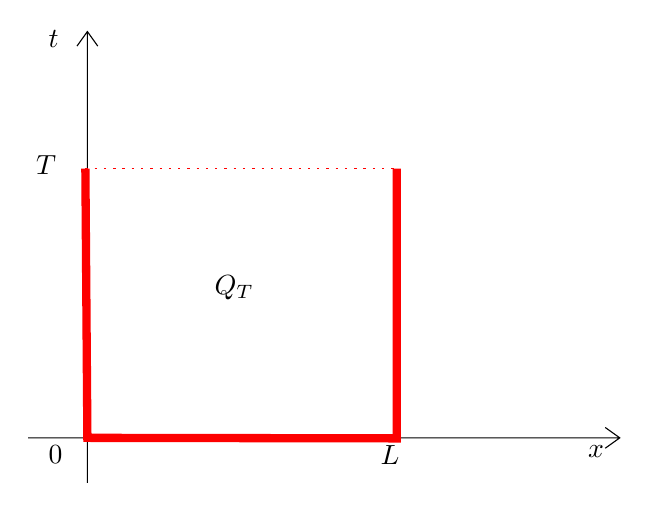
\begin{tikzpicture}[x=0.75pt,y=0.75pt,yscale=-1,xscale=1]
%uncomment if require: \path (0,242); %set diagram left start at 0, and has height of 242

%Shape: Axis 2D [id:dp16320631359033122] 
\draw  (102.47,209.75) -- (387.47,209.75)(130.97,14) -- (130.97,231.5) (380.47,204.75) -- (387.47,209.75) -- (380.47,214.75) (125.97,21) -- (130.97,14) -- (135.97,21)  ;
%Straight Lines [id:da8618748502187668] 
\draw [color={rgb, 255:red, 253; green, 0; blue, 0 } ,draw opacity=1 ][line width=3]    (280,80) -- (280,210) -- (130.97,209.75) -- (130,80) ;
%Straight Lines [id:da3361298498798142] 
\draw [color={rgb, 255:red, 255; green, 0; blue, 0 } ,draw opacity=1 ] [dash pattern={on 0.84pt off 2.51pt}]  (130,80) -- (280,80) ;

% Text Node
\draw (371,212.4) node [anchor=north west][inner sep=0.75pt]    {$x$};
% Text Node
\draw (111,12.4) node [anchor=north west][inner sep=0.75pt]    {$t$};
% Text Node
\draw (191,130.4) node [anchor=north west][inner sep=0.75pt]    {$Q_{T}$};
% Text Node
\draw (111,212.4) node [anchor=north west][inner sep=0.75pt]    {$0$};
% Text Node
\draw (271,212.4) node [anchor=north west][inner sep=0.75pt]    {$L$};
% Text Node
\draw (105,72.4) node [anchor=north west][inner sep=0.75pt]    {$T$};


\end{tikzpicture}

\end{figure}
\FloatBarrier
\end{nb}
In alcuni casi $\displaystyle x$ può variare in intervalli illimitati del tipo $\displaystyle (0,\infty)$ o $\displaystyle \mathbb{R}$ (sbarra ideale infinita). Il problema di Cauchy globale richiede allora delle condizioni aggiuntive che vedremo più avanti

$\displaystyle \begin{cases}
u_{t} -Du_{xx} =f & x\in \mathbb{R},\ 0< t< T\\
u(x,0) =g(x) & x\in \mathbb{R}\\
+\ \mathrm{condizioni\ } x\rightarrow \infty  & 
\end{cases}$


\section{Metodo di separazione delle variabili}

Esaminiamo un modello della sbarra in dimensione n=1. Sotto opportune ipotesi si può dimostrare facilmente che il problema è ben posto utilizzando il metodo di separazione delle variabili. Consideriamo la seguente situazione:
\begin{equation*}
\begin{cases}
u_{t} -Du_{xx} =0 & 0< x< L,\ t >0\\
u(x,0) =u_{0} & 0\leqslant x\leqslant L\\
u(0,t) =u_{0},\ u(L,t) =u_{1} & t >0
\end{cases}
\end{equation*}

Dove $\displaystyle u_{0},u_{1}$ costanti e $\displaystyle u_{1}  >u_{0}$. La sbarra è tenuta dunque inizialmente alla temperatura iniziale costante $\displaystyle u_{0}$. Successivamente, l'estremo $\displaystyle x=0$ mantiene la stessa temperatura (\textbf{estremo freddo}) mentre ho una discontinuità in $\displaystyle x=L$, mantenuto alla temperatura costante $\displaystyle u_{1}$(\textbf{estremo caldo}).

Attraverso un \textbf{ragionamento euristico} possiamo provare a capire come si evolverà la temperatura della sbarra nel tempo: dall'estremo caldo vi sarà un flusso entrante di calore che aumenterà la temperatura della sbarra, dall'estremo freddo un flusso uscente. All'inizio il flusso entrante sarà maggiore del flusso uscente ma, col passare del tempo (e con l'aumento della temperatura della sbarra), il flusso entrante diminuirà e il flusso uscente aumenterà fino a raggiungere una \textbf{situazione stazionaria} con i flussi bilanciati. Poiché siamo interessati al comportamento a regime, $t$ è illimitato.



\textbf{Variabili adimensionali}

Per motivi numerici e modellistici è utile riscrivere il problema di partenza utilizzando delle quantità indipendenti dalle unità di misura, riscalando spazio, tempo e temperatura

\begin{itemize}
\item \textbf{Spazio}: riscalo usando la lunghezza della sbarra $\displaystyle L$ \begin{equation*}
y=x/L,\ 0< y< 1
\end{equation*}
\item \textbf{Tempo}: osserviamo che le dimensioni di $\displaystyle D$ sono\begin{equation*}
[ D] =lunghezza^{2} \times tempo^{-1}
\end{equation*}Definisco $\displaystyle \tau =\frac{L^{2}}{D}$, ha le dimensioni di un tempo e dipende dalle caratteristiche fisiche del problema. Riscalo il tempo usando la costante $\displaystyle \tau $\begin{equation*}
s=t/\tau 
\end{equation*}
\item \textbf{Temperatura}: definisco\begin{equation*}
v(y,s) =\frac{u(Ly,\tau s) -u_{0}}{u_{1} -u_{0}}
\end{equation*}osservo che $\displaystyle v(y,0) =0,\ v(0,s) =0,\ v(1,s) =1,$ inoltre\begin{equation*}
v_{s} =\frac{u_{t} \tau }{u_{1} -u_{0}},\ v_{yy} =\frac{L^{2} u_{xx}}{u_{1} -u_{0}}
\end{equation*}sostituendo $\displaystyle u_{t} =Du_{xx}$ ottengo\begin{equation*}
v_{s} =\frac{L^{2} u_{xx}}{u_{1} -u_{0}}
\end{equation*}
\end{itemize}
$\displaystyle v$ soddisfa l'equazione del calore senza il termine $\displaystyle D$, normalizzato a 1. Posso riscrivere il mio problema in forma adimensionale.

\begin{equation*}
\begin{cases}
v_{s} -v_{yy} =0 & 0< y< 1,s >0\\
v(y,0) =0 & 0< y< 1\\
v(0,s) =0,\ v(1,s) =1 & s >0
\end{cases}
\end{equation*}



\textbf{Condizioni omogenee}

Il problema in forma adimensionale presenta ancora una condizione non omogenea $\displaystyle v(1,s) =1$. Per usare il metodo di separazione delle variabili è necessario che tutto il sistema sia omogeneo. 

Prendiamo in considerazione la soluzione stazionaria, per definizione essa non dipende dal tempo ($\displaystyle v^{st}(y)$) e si dimentica delle condizioni iniziali. Il sistema assume la forma

\begin{equation*}
\begin{cases}
v_{yy} =0 & 0< y< 1\\
v(0) =0,\ v(1) =1 & 
\end{cases}
\end{equation*}

Da cui integrando si ricava 

\begin{equation*}
v^{st}(y) =y
\end{equation*}

\begin{nb}
Ritornando alla forma dimensionale l'equazione diventa
\begin{equation*}
u^{st}(x) =u_{0} +(u_{1} -u_{0})\frac{x}{L}
\end{equation*}
La soluzione stazionaria corrisponde dunque ad un flusso uniforme di calore lungo la sbarra del valore 
\begin{equation*}
\text{flusso} =-\frac{k}{L}(u_{1} -u_{0})
\end{equation*}
\end{nb}



Definendo a questo punto il \textbf{regime transitorio:}

\begin{equation*}
U(y,s) =v^{st}(y) -v(y,s) =y-v(y,s)
\end{equation*}
esso tenderà a 0 per $\displaystyle s\rightarrow \infty $. $\displaystyle U$ soddisfa ancora l'equazione del calore e posso riscrivere il sistema con condizioni omogenee
\begin{equation*}
\boxed{\begin{cases}
U_{s} -U_{yy} =0 & 0< y< 1,\ s >0\\
U(0,s) =U(1,s) =0 & s >0\\
U(y,0) =y & 0\leqslant y\leqslant 1
\end{cases}}
\end{equation*}
\textbf{Applicazione del metodo}

Ora che il problema è nella forma adatta voglio costruire una soluzione non banale mediante sovrapposizione di soluzioni particolari della forma

\begin{equation*}
U(y,s) =w(s) v(y)
\end{equation*}

in modo tale che $\displaystyle v(0) =v(1) =0$

Sostituendo la forma della soluzione nell'equazione del calore ottengo

\begin{equation*}
w'(s) v(y) -w(s) v'' (y) =0,\ \forall y\in (0,1),\ \forall s >0
\end{equation*}
Da cui dividendo per $\displaystyle w(s) v(y)$ e separando:
\begin{equation*}
\frac{w'(s)}{w(s)} =\frac{v'' (y)}{v(y)} =\lambda 
\end{equation*}
Dove $\displaystyle \lambda $ è una costante: infatti perché l'identità tra i due rapporti sia valida per ogni $\displaystyle s >0$ ed ogni $\displaystyle y\in (0,1)$, essendo il primo membro funzione della sola variabile $\displaystyle s$ ed il secondo della sola variabile $\displaystyle y$, l'unica possibilità è che siano entrambi uguali ad una costante comune. Posso dividere il mio problema iniziale in due sottoproblemi
\begin{itemize}
\item \textbf{Problema 1}\begin{equation*}
\begin{cases}
v'' (y) -\lambda v(y) =0\\
v(0) =v(1) =0
\end{cases}
\end{equation*}

Si presentano 3 casi
\begin{itemize}
\item $\displaystyle \lambda  >0$, l'integrale generale è $\displaystyle v(y) =c_{1} e^{\sqrt{\lambda } y} +c_{2} e^{-\sqrt{\lambda } y}$, le condizioni al bordo\begin{equation*}
\begin{cases}
v(0) =c_{1} +c_{2} =0\\
v(1) =c_{1} e^{\sqrt{\lambda }} +c_{2} e^{-\sqrt{\lambda }} =0
\end{cases}
\end{equation*}da cui $\displaystyle c_{1} =c_{2} =0$, per cui otteniamo soluzioni banali
\item $\displaystyle \lambda =0$, l'integrale generale è $\displaystyle v(y) =c_{1} y+c_{2}$, che unito alle condizioni al bordo dà $\displaystyle c_{1} =c_{2} =0$, soluzioni banali
\item $\displaystyle \lambda =-\mu ^{2} < 0$, l'integrale generale è $\displaystyle v(y) =c_{1}\cos(\mu y) +c_{2}\sin(\mu y)$, le condizioni al bordo\begin{equation*}
\begin{cases}
v(0) =c_{1} =0\\
v(1) =c_{1}\cos(\mu) +c_{2}\sin(\mu) =c_{2}\sin(\mu) =0
\end{cases}
\end{equation*}

Escludendo le soluzioni banali ($\displaystyle c_{2} =0$) ottengo $\displaystyle \sin(\mu) =0$ e quindi $\displaystyle \mu =m\pi,\ m=1,2..$ 
\end{itemize}

Le soluzioni non banali del \textbf{problema 1} sono della forma\footnote{$\displaystyle v_{m}$ prendono il nome di autofunzioni e $\displaystyle \lambda _{m}$ di autovalori}\begin{equation*}
\boxed{v_{m}(y) =c_{2}\sin(m\pi y),\ \lambda _{m} =-m^{2} \pi ^{2}}
\end{equation*}


\item \textbf{Problema 2}\begin{equation*}
w'(s) =\lambda w(s)
\end{equation*}

Ha soluzioni non banali della forma\begin{equation*}
\boxed{w_{m}(s) =Ce^{\lambda _{m} s} =Ce^{-m^{2} \pi ^{2} s}}
\end{equation*}
\end{itemize}



Unendo le soluzioni dei due problemi ottengo infinite soluzioni numerabili
\begin{equation*}
U_{m}(y,s) =A_{m} e^{-m^{2} \pi ^{2} s}\sin(m\pi y) \ \ \ \ m=1,2,\dotsc 
\end{equation*}
\textit{Lezione 5 2/3/2021}

Nessuna di queste infinite soluzioni soddisfa la condizione iniziale $U(y,0) =y$, cerchiamo quindi di ottenere ciò che vogliamo sovrapponendo le infinite soluzioni
\begin{equation*}
\boxed{U(y,s) =\sum\limits ^{\infty }_{m=1} A_{m} e^{-m^{2} \pi ^{2} s}\sin(m\pi y)}
\end{equation*}
Imponiamo la condizione iniziale, per farlo risulta
\begin{equation}
U(y,0) =\sum\limits ^{\infty }_{m=1} A_{m}\sin(m\pi y) =y
\label{eq:diff-cond-iniziale}
\end{equation}
quell'uguaglianza ad $y$ è da intendersi nel senso $L^{2}$, nello specifico dobbiamo sviluppare la funzione $f(y) =y$ in serie di Fourier nell'intervallo $(0,1)$ per calcolare i coefficienti che garantiscono la condizione iniziale.



Considerando una generica funzione $T$-periodica, si scrive in \textbf{serie di Fourier}\footnote{Il simbolo $\sim $ indica che l'uguaglianza vale nel senso $L^{2}\left( -\frac{T}{2},\frac{T}{2}\right)$. Indicando con $S_{N}(y)$ le somme parziali della serie, vale
\begin{equation*}
\lim _{N\rightarrow \infty }\int ^{T/2}_{-T/2}[ f(y) -S_{N}(y)]^{2} dy=0
\end{equation*}}
\begin{equation*}
f(y) \sim \frac{a_{0}}{2} +\sum\limits ^{\infty }_{m=1}\left[ a_{m}\cos\left(\frac{2\pi m}{T} y\right) +b_{m}\sin\left(\frac{2\pi m}{T} y\right)\right]
\end{equation*}
i cui coefficienti sono, per $m\geqslant 0$
\begin{equation*}
a_{m} =\frac{2}{T}\int ^{T/2}_{-T/2} f(y)\cos\left(\frac{2\pi m}{T} y\right) dy\ \ \ \ b_{m} =\frac{2}{T}\int ^{T/2}_{-T/2} f(y)\sin\left(\frac{2\pi m}{T} y\right) dy
\end{equation*}
Ricordiamo l'\textbf{identità di Parseval}
\begin{equation*}
\frac{2}{T}\int ^{T/2}_{-T/2}[ f(y)]^{2} dy=\frac{a^{2}_{0}}{2} +\sum\limits ^{\infty }_{m=1}\left( a^{2}_{m} +b^{2}_{m}\right)
\end{equation*}
Nel nostro caso vogliamo sviluppare la funzione $2$-periodica
\begin{equation*}
f:[ -1,1]\rightarrow \mathbb{R} \ \ f(y) =y
\end{equation*}
È dispari traslata, quindi è composta da soli seni
\begin{align*}
b_{m} & =\int ^{1}_{-1} y\sin(m\pi y) dy=2\int ^{1}_{0} y\sin(m\pi y) dy\\
 & \overset{\text{ipp}}{=}\left[ -\frac{2}{m\pi } y\cos(m\pi y)\right]^{1}_{0} +\frac{2}{m\pi }\int ^{1}_{0}\cos(m\pi y) dy\\
 & =-2\frac{\cos(m\pi)}{m\pi } +\cancel{\frac{2}{m^{2} \pi ^{2}}[\sin(m\pi y)]^{1}_{0}} =\frac{2}{\pi }\frac{(-1)^{m+1}}{m}
\end{align*}
allora
\begin{equation}
y\sim \sum\limits ^{\infty }_{m=1}\left[\frac{2}{\pi }\frac{(-1)^{m+1}}{m}\sin(m\pi y)\right]
\label{eq:diff-y-fourier}
\end{equation}
Lo sviluppo è valido nell'intervallo $(-1,1)$, agli estremi è nulla, e converge uniformemente in ogni $[ a,b] \subset (-1,1)$.

La nostra soluzione \textit{candidata} è quindi, a seguito di \eqref{eq:diff-cond-iniziale} e \eqref{eq:diff-y-fourier} uguagliando i coefficienti
\begin{equation}
\boxed{U(y,s) =\sum\limits ^{\infty }_{m=1}\frac{2}{\pi }\frac{(-1)^{m+1}}{m}\sin(m\pi y) e^{-m^{2} \pi ^{2} s}}
\label{eq:diff-candidata}
\end{equation}
\textbf{Questioni aperte}
\begin{itemize}
\item \textbf{Q1} \textit{Condizione iniziale.} In che senso\begin{equation*}
U(y,s)\rightarrow y\ \text{per} \ s\rightarrow 0^{+}
\end{equation*}
\item \textbf{Q2} Le $U_{m}$ sono tutte soluzioni dell'equazione del calore. Anche $U$ lo sarà? Se possiamo scambiare derivata e serie allora sì\begin{equation*}
( \partial _{s} -\partial _{yy}) U(y,s)\overset{?}{=}\sum ^{\infty }_{m=1}( \partial _{s} -\partial _{yy}) U_{m} (y,s)=0
\end{equation*}
\item \textbf{Q3} $U$ soddisfa la \textit{condizione al bordo}?\begin{gather*}
\lim\limits _{(y,s)\rightarrow (0,s_{0})} U(y,s) =0\\
\lim\limits _{(y,s)\rightarrow (1,s_{0})} U(y,s) =0
\end{gather*}
\item \textbf{Q4} \textit{Unicità.}
\item \textbf{Q5} È vero che $U(y,s)\rightarrow 0$ se $s\rightarrow \infty $?
\end{itemize}

\textbf{Risposte}
\begin{itemize}
\item \textbf{Q1} Consideriamo \eqref{eq:diff-candidata} e \eqref{eq:diff-y-fourier}. Per Parseval\begin{gather*}
\int ^{1}_{0}[ U(y,s) -y]^{2} dy=\frac{2}{\pi ^{2}}\sum\limits ^{\infty }_{m=1}\frac{\left( e^{-m^{2} \pi ^{2} s} -1\right)^{2}}{m^{2}}\\
\Rightarrow \ \ \frac{\left( e^{-m^{2} \pi ^{2} s} -1\right)^{2}}{m^{2}} \leqslant \frac{1}{m^{2}} \ \text{per} \ s\geqslant 0
\end{gather*}

Allora la serie converge uniformemente per il test di Weierstrass in $[ 0,+\infty)$ rispetto ad $s$, quindi\begin{equation*}
U(y,s) -y\rightarrow 0\ \text{in senso} \ L^{2}(0,1) \ \text{se} \ s\rightarrow 0
\end{equation*}
\item \textbf{Q2} Consideriamo \eqref{eq:diff-candidata}. Consideriamo una semistriscia del tipo\begin{equation*}
[ 0,1] \times [ s_{0},+\infty) \ \ s_{0}  >0
\end{equation*}

Il termine generale della serie $\sum U_{m}$ in modulo è maggiorato da\begin{equation*}
\left| \frac{(-1)^{m+1}}{m}\sin(m\pi y) e^{-m^{2} \pi ^{2} s}\right| \leqslant e^{-m^{2} \pi ^{2} s_{0}} \ \ \text{se} \ s >s_{0}
\end{equation*}

quindi per il test di Weierstrass la serie converge uniformemente.

Inoltre la serie delle derivate $\sum \partial _{s} U_{m},\sum \partial _{yy} U_{m}$ converge uniformemente sempre per il test di Weierstrass\begin{gather*}
\frac{\partial U_{m}}{\partial s} =\frac{\partial ^{2} U_{m}}{\partial y^{2}} =(-1)^{m+2} 2m\pi e^{-m^{2} \pi ^{2} s}\sin(m\pi y)\\
\Rightarrow \ \ \left| \frac{\partial U_{m}}{\partial s}\right| =\left| \frac{\partial ^{2} U_{m}}{\partial y^{2}}\right| \leqslant 2m \pi e^{-m^{2} \pi ^{2} s_{0}},\ \ s\geqslant s_{0} \ \text{nella striscia}
\end{gather*}

Quindi possiamo scambiare serie e derivata e $U(y,s)$ è anch'essa soluzione.

Deduciamo anche che\begin{equation*}
U\in C^{\infty }([ 0,1] \times (0,+\infty))
\end{equation*}

avevamo una discontinuità nell'estremo destro, ma è diventata \textit{istantaneamente} regolare. Questo è l'\textbf{effetto regolarizzante} dell'equazione del calore.
\item \textbf{Q3} Sì perché la serie di $U$ è uniformemente convergente in $[ 0,1] \times [ s_{0},+\infty)$, $\forall s_{0}  >0$ e possiamo scambiare serie e limite.
\item \textbf{Q4} Usiamo il \textit{metodo dell'energia.}

Supponiamo che esistano due soluzioni nella stessa classe di $U$ con lo stesso dato iniziale $y$, assunto in senso $L^{2}(0,1)$. Poniamo\begin{equation*}
w=U-V
\end{equation*}

vogliamo mostrare che $w$ è nulla. La $w$ è soluzione dell'equazione con dati iniziali e al bordo nulli\begin{equation*}
\begin{cases}
w_{s} -w_{yy} =0, & \text{in} \ 0< y< 1,s >0\\
w(0,s) =w(1,s) =0, & \boxed{s >0}\\
w(y,0) =0, & \text{in senso} \ L^{2}(0,1)
\end{cases}
\end{equation*}

 Moltiplichiamo per $w$ da entrambi i lati e integriamo\begin{gather*}
\textcolor[rgb]{0.82,0.01,0.11}{\int ^{1}_{0}}\textcolor[rgb]{0.82,0.01,0.11}{ww}\textcolor[rgb]{0.82,0.01,0.11}{_{s}}\textcolor[rgb]{0.82,0.01,0.11}{dy} =\textcolor[rgb]{0.29,0.56,0.89}{\int ^{1}_{0}}\textcolor[rgb]{0.29,0.56,0.89}{ww}\textcolor[rgb]{0.29,0.56,0.89}{_{yy}}\textcolor[rgb]{0.29,0.56,0.89}{dy}\\
\begin{aligned}
\textcolor[rgb]{0.82,0.01,0.11}{\int ^{1}_{0}}\textcolor[rgb]{0.82,0.01,0.11}{ww}\textcolor[rgb]{0.82,0.01,0.11}{_{s}}\textcolor[rgb]{0.82,0.01,0.11}{dy} & =\frac{1}{2}\int ^{1}_{0}\frac{\partial }{\partial s} w^{2}(y,s) dy=\frac{1}{2}\frac{d}{ds}\underbrace{\int ^{1}_{0} w^{2}(y,s) dy}_{E(s)} =\frac{1}{2} E'(s)\\
\textcolor[rgb]{0.29,0.56,0.89}{\int ^{1}_{0}}\textcolor[rgb]{0.29,0.56,0.89}{ww}\textcolor[rgb]{0.29,0.56,0.89}{_{yy}}\textcolor[rgb]{0.29,0.56,0.89}{dy} & \overset{\text{ipp}}{=}\cancel{ww_{y} |^{1}_{0}} -\int ^{1}_{0}(w_{y})^{2} dy\leqslant 0
\end{aligned}
\end{gather*}

quindi $E(s)$ è non negativa, descrescente (non strettamente), inoltre $E(s)\rightarrow 0$ se $s\rightarrow 0$, allora\begin{equation*}
E(s) =0\ \ \forall s >0\ \ \Rightarrow \ \ \int ^{1}_{0} w^{2}(y,s) dy=0\ \ \forall s >0
\end{equation*}

ma $w^{2}$ è continua per $s >0$ e non negativa. Non può essere che $w=0$ per $s >0$, ovvero $U=V$.
\item \textbf{Q5} Sempre per la convergenza uniforme della serie: se $\displaystyle s\geqslant 1$, il termine generale \begin{equation*}
\left| \frac{(-1)^{m+1}}{m}\sin(m\pi y) e^{-m^{2} \pi ^{2} s}\right| \leqslant \frac{e^{-m^{2} \pi ^{2}}}{m}
\end{equation*}

quindi per il test di Weierstrass la serie converge uniformemente in $\displaystyle [ 0,1] \times [ 1,\infty)$, posso passare al limite sotto il segno di somma: $\displaystyle U(y,s) =\sum\limits ^{\infty }_{m=1}\frac{2}{\pi }\frac{(-1)^{m+1}}{m}\sin(m\pi y) e^{-m^{2} \pi ^{2} s}\xrightarrow{s\rightarrow \infty } 0$ uniformemente per $\displaystyle y\in [ 0,1]$
\end{itemize}



\textbf{Ritorno alle origini.}

Avevamo definito\begin{equation*}
v(y,s) =\frac{u(Ly,\tau s) -u_{0}}{u_{1} -u_{0}} \ \ \Rightarrow \ \ u(Ly,\tau s) =u_{0} +[ u_{1} -u_{0}] v(y,s)
\end{equation*}

e anche
\begin{equation*}
v(y,s) =y-U(y,s) \ \ \ \ s=\frac{t}{\tau } \ \ \ \ y=\frac{x}{L} \ \ \ \ \tau =\frac{L^{2}}{D}
\end{equation*}
da cui possiamo riscrivere la soluzione nelle variabili originali
\begin{align*}
u(x,t) & =u_{0} +[ u_{1} -u_{0}](y-U(y,s))\\
 & =u_{0} +[ u_{1} -u_{0}] y-[ u_{1} -u_{0}] U(y,s)\\
 & =u_{0} +[ u_{1} -u_{0}]\frac{x}{L} -[ u_{1} -u_{0}]\sum\limits ^{\infty }_{m=1}\frac{2}{\pi }\frac{(-1)^{m+1}}{m} e^{-m^{2} \pi ^{2}\textcolor[rgb]{0.82,0.01,0.11}{\frac{D}{L^{2}}}\textcolor[rgb]{0.82,0.01,0.11}{t}}\sin\left(\frac{m\pi }{L} x\right)
\end{align*}
A regime notiamo che la supposizione iniziale era corretta, la temperatura si assesta a una soluzione stazionaria fatta come una retta
\begin{equation*}
u(x,t) =u_{0} +[ u_{1} -u_{0}]\frac{x}{L} -\underbrace{[ u_{1} -u_{0}]\sum\limits ^{\infty }_{m=1}\frac{2}{\pi }\frac{(-1)^{m+1}}{m} e^{-m^{2} \pi ^{2}\frac{D}{L^{2}} t}\sin\left(\frac{m\pi }{L} x\right)}_{\rightarrow 0\ \text{per} \ t\rightarrow \infty }
\end{equation*}

\fg{0.7}{diffusione-soluzione-1d}

\section{Problemi in dimensione \texorpdfstring{$n>1$}{n > 1}}

Sia $\displaystyle \Omega $ un dominio\footnote{ovvero un aperto connesso in $\displaystyle \mathbb{R}^{n}$.}. La temperatura sarà una $u=u(\mathbf{x},t)$ che soddisfa $u_{t} -D\Delta u=f$ nel \textit{cilindro spazio-temporale}
\begin{equation*}
Q_{T} =\Omega \times (0,T)
\end{equation*}

\fg{0.7}{diffusione-problema-2d}

Occorre assegnare
\begin{itemize}
\item \textit{condizione iniziale}\begin{equation*}
u(\mathbf{x},0) =g(\mathbf{x}) \ \ \mathbf{x} \in \overline{\Omega }
\end{equation*}
\item \textit{condizioni sul bordo} $\partial \Omega $
\begin{itemize}
\item \textbf{Dirichlet}, si assegna la temperatura\begin{equation*}
u(\mathbf{\sigma },t) =h(\mathbf{\sigma },t) \ \ \ \ \mathbf{\sigma } \in \partial \Omega,t\in ( 0,T]
\end{equation*}
\item \textbf{Neumann}, si assegna il flusso attraverso $\partial \Omega $. Indichiamo con $\mathbf{\nu }$ il versore normale al bordo in funzione del punto. Ricordiamo che $\partial _{\mathbf{\nu }} u=\nabla u\cdotp \mathbf{\nu }$. Si assegna\begin{equation}
\partial _{\mathbf{\nu }}(\mathbf{\sigma },t) =h(\mathbf{\sigma },t) \ \ \ \ \mathbf{\sigma } \in \partial \Omega,t\in ( 0,T]
\end{equation}
\item \textbf{Robin}, si assegna $(\alpha  >0)$\begin{equation*}
\partial _{\mathbf{\nu }} u(\mathbf{\sigma },t) +\alpha u(\mathbf{\sigma },t) =\beta \ \ \ \ \mathbf{\sigma } \in \partial \Omega,t\in ( 0,T]
\end{equation*}
\end{itemize}
\end{itemize}

Le condizioni al bordo possono essere miste, per esempio $\partial \Omega =\gamma _{1} \cup \gamma _{2}$ e possiamo avere una condizione su $\gamma _{1}$ e una diversa condizione su $\gamma _{2}$.

Il problema è quindi determinare $u$ tale che
\begin{equation*}
\begin{cases}
u_{t} -D\Delta u=f & \text{in} \ Q_{T}\\
u(\mathbf{x},0) =g(\mathbf{x}) & \text{in} \ \overline{\Omega }\\
+\ \text{condizioni al bordo} & \text{su} \ \partial \Omega \times ( 0,T]
\end{cases}
\end{equation*}
\textbf{Problema di Cauchy globale.}
\begin{equation*}
\begin{cases}
u_{t} -D\Delta u=f & \mathbf{x} \in \mathbb{R}^{n},0< t< T\\
u(\mathbf{x},0) =g(\mathbf{x}) & \mathbf{x} \in \mathbb{R}^{n}\\
\mathrm{+\ condizioni\ all'\infty } & 
\end{cases}
\end{equation*}
\begin{definition}
[Frontiera parabolica] Le condizioni sono assegnate sulla frontiera parabolica del cilindro, cioè l'unione della base e della parte laterale $S_{T} =\partial \Omega \times ( 0,T]$
\begin{equation*}
\partial _{p} Q_{T} =(\overline{\Omega } \times \{t=0\}) \cup S_{T}
\end{equation*}
\end{definition}
\section{Principi di massimo}

Il calore fluisce verso regioni dove la temperatura è più bassa, da ciò segue che la soluzione omogenea assume massimi e minimi globali sulla frontiera parabolica. Inoltre, risente di una irreversibilità temporale, il futuro non influenza il passato.

Indichiamo con $C^{2,1}(Q_{T})$ l'insieme delle funzioni di classe
\begin{equation*}
\begin{array}{ l l }
C^{2} & \text{rispetto a} \ x\\
C^{1} & \text{rispetto a} \ t
\end{array}
\end{equation*}
\textit{su misura} per l'equazione del calore.
\begin{theorem}
[Principio di massimo debole] Sia $Q_{T} =\Omega \times (0,T)$, $\Omega $ dominio limitato. Sia $u\in C^{2,1}(Q_{T}) \cap C(\overline{Q}_{T})$ tale che
\begin{equation*}
u_{t} -D\Delta u=q\leqslant 0\ \ \text{in} \ Q_{T} \ \ \left(\text{risp.} \ \geqslant 0\right)
\end{equation*}
Allora il massimo (risp. minimo) di $u$ è assunto sulla frontiera parabolica di $Q_{T}$
\begin{equation*}
\max_{\overline{Q}_{T}} u=\max_{\partial _{p} Q_{T}} u\ \ \ \ \left(\text{risp.} \ \min_{\overline{Q}_{T}} u=\min_{\partial _{p} Q_{T}} u\right)
\end{equation*}
\end{theorem}
\begin{dimostrazione}
Sia $w=u-\varepsilon t$, allora
\begin{equation}
w_{t} -D\Delta w=q-\varepsilon < 0
\label{eq:max-deb-contr-1}
\end{equation}
Affermo che
\begin{equation*}
\max_{\overline{Q}_{T-\varepsilon }} w=\max_{\partial _{p} Q_{T-\varepsilon }} w
\end{equation*}



\begin{figure}[H]
	\centering

\tikzset{every picture/.style={line width=0.75pt}} %set default line width to 0.75pt        

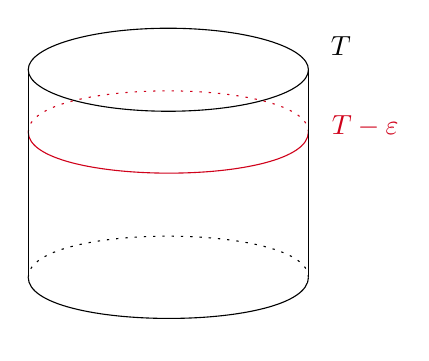
\begin{tikzpicture}[x=0.75pt,y=0.75pt,yscale=-1,xscale=1]
%uncomment if require: \path (0,160); %set diagram left start at 0, and has height of 160

%Shape: Ellipse [id:dp9954583197247324] 
\draw   (163,30) .. controls (163,18.95) and (193.22,10) .. (230.5,10) .. controls (267.78,10) and (298,18.95) .. (298,30) .. controls (298,41.05) and (267.78,50) .. (230.5,50) .. controls (193.22,50) and (163,41.05) .. (163,30) -- cycle ;
%Curve Lines [id:da36272626169586997] 
\draw    (163,130) .. controls (163,156.25) and (297.8,156.6) .. (298,130) ;
%Curve Lines [id:da5257514313993306] 
\draw  [dash pattern={on 0.84pt off 2.51pt}]  (298,130) .. controls (298,103.75) and (163.2,103.4) .. (163,130) ;
%Curve Lines [id:da6861700154443668] 
\draw [color={rgb, 255:red, 208; green, 2; blue, 27 } ,draw opacity=1 ]   (163,60) .. controls (163,86.25) and (297.8,86.6) .. (298,60) ;
%Curve Lines [id:da46362431718689145] 
\draw [color={rgb, 255:red, 208; green, 2; blue, 27 } ,draw opacity=1 ] [dash pattern={on 0.84pt off 2.51pt}]  (298,60) .. controls (298,33.75) and (163.2,33.4) .. (163,60) ;
%Straight Lines [id:da3476763854948828] 
\draw    (163,30) -- (163,130) ;
%Straight Lines [id:da7597497497420163] 
\draw    (298,30) -- (298,130) ;

% Text Node
\draw (307.5,12.9) node [anchor=north west][inner sep=0.75pt]    {$T$};
% Text Node
\draw (308,50.9) node [anchor=north west][inner sep=0.75pt]  [color={rgb, 255:red, 208; green, 2; blue, 27 } ,opacity=1 ]  {$T-\varepsilon $};


\end{tikzpicture}

\end{figure}
\FloatBarrier

Se non fosse vero esisterebbe $(x_{0},t_{0}) \in \overline{Q}_{T-\varepsilon } \setminus \partial _{p} Q_{T-\varepsilon }$ punto di massimo per $w$, tale punto può trovarsi o all'interno o sul tappo superiore
\begin{equation*}
\begin{array}{ l l l }
\text{all'interno} & w_{t} =0 & \Delta w\leqslant 0\\
\text{sul tappo} & w_{t} \geqslant 0 & \Delta w\leqslant 0
\end{array}
\end{equation*}
in entrambi i casi
\begin{equation}
w_{t} -D\Delta w\geqslant 0
\label{eq:max-deb-contr-2}
\end{equation}
le \eqref{eq:max-deb-contr-1} e \eqref{eq:max-deb-contr-2} sono in contraddizione, quindi è vero.

Inoltre $w\leqslant u$ e $u=w+\varepsilon t\leqslant w+\varepsilon T$
\begin{align*}
\max_{\overline{Q}_{T-\varepsilon }} u & \leqslant \max_{\overline{Q}_{T-\varepsilon }} w+\varepsilon T\\
 & =\max_{\partial _{p} Q_{T-\varepsilon }} w+\varepsilon T\\
 & \leqslant \max_{\partial _{p} Q_{T-\varepsilon }} u+\varepsilon T
\end{align*}
Facendo tendere $\varepsilon \rightarrow 0$
\begin{equation*}
\max_{\overline{Q}_{T}} u\leqslant \max_{\partial _{p} Q_{T}} u
\end{equation*}
d'altro canto, essendo l'insieme a destra compreso in quello di sinistra, il massimo di sinistra deve essere almeno tanto quanto quello di destra
\begin{equation*}
\max_{\overline{Q}_{T}} u\geqslant \max_{\partial _{p} Q_{T}} u
\end{equation*}
da cui la tesi.
\end{dimostrazione}
\textit{Lezione 6 (8/3/2021)}
\section{Conseguenze del principio di massimo debole}

Sia $u\in C^{1,2}(Q_{T}) \cap C(\overline{Q}_{T})$ soluzione di
\begin{equation*}
u_{t} -D\Delta u=0\ \ \text{in} \ Q_{T}
\end{equation*}
allora
\begin{equation*}
\min_{\partial _{p} Q_{T}} u\leqslant \min_{\overline{Q}_{T}} u\leqslant \max_{\overline{Q}_{T}} u\leqslant \max_{\partial _{p} Q_{T}} u
\end{equation*}
\subsection{Corollario del massimo debole}

Siano $f_{1},f_{2}$ funzioni limitate in $Q_{T}$ e $u,v$ soluzioni di
\begin{gather*}
u_{t} -D\Delta u=f_{1}\\
v_{t} -D\Delta v=f_{2}
\end{gather*}
Allora
\begin{enumerate}
\item \textit{Confronto.} Se $f_{1} \leqslant f_{2}$ in $Q_{T}$ e $u\leqslant v$ su $\partial _{p} Q_{T}$ allora\begin{equation*}
u\leqslant v\ \text{in tutto} \ Q_{T}
\end{equation*}
\item Vale la stima\begin{equation*}
\max_{\overline{Q}_{T}}| u-v| \leqslant \max_{\partial _{p} Q_{T}}| u-v| +T\sup _{Q_{T}}| f_{1} -f_{2}| 
\end{equation*}

È una stabilità in norma $L^{\infty }$\begin{equation*}
\Vert u-v\Vert _{L^{\infty }(\overline{Q}_{T})} \leqslant \Vert u-v\Vert _{L^{\infty }( \partial _{p} Q_{T})} +T\Vert f_{1} -f_{2}\Vert _{L^{\infty }(Q_{T})}
\end{equation*}

Questo implica l'\textbf{unicità per il problema di Cauchy-Dirichlet} in $C^{1,2}(Q_{T}) \cap C(\overline{Q}_{T})$. Stessi dati sulla frontiera e stessa sorgente esogena, allora $u=v$, infatti
\begin{enumerate}
\item Sia $u$ soluzione di\begin{equation*}
\begin{cases}
u_{t} -D\Delta u=f & \text{in} \ Q_{T}\\
u=h & \text{su} \ S_{T}\\
u=g & \text{per} \ t=0\ \text{in} \ \overline{\Omega }
\end{cases}
\end{equation*}se $v$ è un'altra soluzione allora $w=u-v$ soddisfa\begin{equation*}
\begin{cases}
w_{t} -D\Delta w=f & \text{in} \ Q_{T}\\
w=0 & \text{su} \ S_{T}\\
w=0 & \text{per} \ t=0\ \text{in} \ \overline{\Omega }
\end{cases}
\end{equation*}allora abbiamo\begin{equation*}
\Vert w\Vert _{L^{\infty }(\overline{Q}_{T})} \leqslant 0+0\ \ \Rightarrow \ \ u=v
\end{equation*}
\end{enumerate}
\end{enumerate}
\subsection{Principio di massimo forte}

Perché si chiama principio di massimo debole?

Se prendiamo un problema del tipo



\begin{figure}[htpb]
	\centering

\tikzset{every picture/.style={line width=0.75pt}} %set default line width to 0.75pt        

\begin{tikzpicture}[x=0.75pt,y=0.75pt,yscale=-1,xscale=1]
%uncomment if require: \path (0,297); %set diagram left start at 0, and has height of 297

%Straight Lines [id:da3946008733456672] 
\draw    (200,214.31) -- (508,214.31) ;
\draw [shift={(510,214.31)}, rotate = 180] [fill={rgb, 255:red, 0; green, 0; blue, 0 }  ][line width=0.08]  [draw opacity=0] (12,-3) -- (0,0) -- (12,3) -- cycle    ;
%Straight Lines [id:da3125287839949542] 
\draw    (200,214.31) -- (200,20.31) ;
\draw [shift={(200,18.31)}, rotate = 450] [fill={rgb, 255:red, 0; green, 0; blue, 0 }  ][line width=0.08]  [draw opacity=0] (12,-3) -- (0,0) -- (12,3) -- cycle    ;
%Straight Lines [id:da35837250143803123] 
\draw    (200,58.31) -- (370,58.31) ;
%Straight Lines [id:da9781100684099335] 
\draw    (200,118.31) -- (370,118.31) ;
%Curve Lines [id:da007305458198421322] 
\draw    (138,247.31) .. controls (142.9,210.07) and (163.17,180.52) .. (189.39,164.29) ;
\draw [shift={(191,163.31)}, rotate = 509.35] [fill={rgb, 255:red, 0; green, 0; blue, 0 }  ][line width=0.08]  [draw opacity=0] (12,-3) -- (0,0) -- (12,3) -- cycle    ;
%Curve Lines [id:da5491813976204125] 
\draw    (183,265.31) .. controls (208.74,263.33) and (244.28,250.57) .. (280.89,225.09) ;
\draw [shift={(282,224.31)}, rotate = 504.9] [fill={rgb, 255:red, 0; green, 0; blue, 0 }  ][line width=0.08]  [draw opacity=0] (12,-3) -- (0,0) -- (12,3) -- cycle    ;
%Curve Lines [id:da8634803668913487] 
\draw    (185,281.31) .. controls (377.04,309.17) and (475.02,248.92) .. (384.38,174.44) ;
\draw [shift={(383,173.31)}, rotate = 398.88] [fill={rgb, 255:red, 0; green, 0; blue, 0 }  ][line width=0.08]  [draw opacity=0] (12,-3) -- (0,0) -- (12,3) -- cycle    ;
%Straight Lines [id:da3716594049457218] 
\draw    (370,214.31) -- (370,58.31) ;
%Curve Lines [id:da18228789256355693] 
\draw    (377.19,90.81) .. controls (394.92,86.66) and (417.92,78.71) .. (440,64.31) ;
\draw [shift={(375,91.31)}, rotate = 347.47] [fill={rgb, 255:red, 0; green, 0; blue, 0 }  ][line width=0.08]  [draw opacity=0] (12,-3) -- (0,0) -- (12,3) -- cycle    ;
%Curve Lines [id:da1615187343378126] 
\draw    (182.81,87.81) .. controls (165.08,83.66) and (142.08,75.71) .. (120,61.31) ;
\draw [shift={(185,88.31)}, rotate = 192.53] [fill={rgb, 255:red, 0; green, 0; blue, 0 }  ][line width=0.08]  [draw opacity=0] (12,-3) -- (0,0) -- (12,3) -- cycle    ;

% Text Node
\draw (184,5.4) node [anchor=north west][inner sep=0.75pt]    {$t$};
% Text Node
\draw (179,48.4) node [anchor=north west][inner sep=0.75pt]    {$T$};
% Text Node
\draw (179,105.4) node [anchor=north west][inner sep=0.75pt]    {$\frac{\pi }{2}$};
% Text Node
\draw (125,255.4) node [anchor=north west][inner sep=0.75pt]    {$u=1$};
% Text Node
\draw (512,217.71) node [anchor=north west][inner sep=0.75pt]    {$x$};
% Text Node
\draw (187,217.4) node [anchor=north west][inner sep=0.75pt]    {$0$};
% Text Node
\draw (372,217.71) node [anchor=north west][inner sep=0.75pt]    {$L$};
% Text Node
\draw (445,48.4) node [anchor=north west][inner sep=0.75pt]    {$u=\sin t$};
% Text Node
\draw (75,37.4) node [anchor=north west][inner sep=0.75pt]    {$u=\sin t$};
% Text Node
\draw (240,138.4) node [anchor=north west][inner sep=0.75pt]    {$u_{t} -u_{xx} =0$};
% Text Node
\draw (254,175.4) node [anchor=north west][inner sep=0.75pt]    {$\text{qui} \ u=1$};


\end{tikzpicture}

\end{figure}
\FloatBarrier

$u=1$ per $0\leqslant t\leqslant \pi /2$

Il massimo di $u$ sulla frontiera parabolica è
\begin{equation*}
\max_{\partial _{p} Q_{T}} u=1
\end{equation*}
e il massimo di $u$ su tutto è
\begin{equation*}
\max_{\overline{Q}_{T}} u=1
\end{equation*}
Ma nel rettangolo fino a che $t=\pi /2$ il massimo non è assunto solo sulla frontiera, ma anche tutto all'interno. Si dimostra che è l'unica possibilità affinché avvenga, ovvero che \textbf{il massimo può essere assunto all'interno se fino a quel punto }$u$\textbf{ è rimasto costante (Principio di Massimo Forte).}
\section{Soluzione fondamentale \texorpdfstring{$n=1$}{n = 1}}

In $x=0$ sia concentrata una sorgente di calore \textbf{istantanea.} Indichiamo con $u^{\star }$ la temperatura della sbarra, vogliamo determinare l'evoluzione di $u^{\star },t\geqslant 0$.



\begin{figure}[htpb]
	\centering

\tikzset{every picture/.style={line width=0.75pt}} %set default line width to 0.75pt        

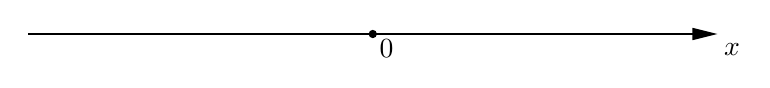
\begin{tikzpicture}[x=0.75pt,y=0.75pt,yscale=-1,xscale=1]
%uncomment if require: \path (0,40); %set diagram left start at 0, and has height of 40

%Straight Lines [id:da34140184544932506] 
\draw    (130,13) -- (460,13) ;
\draw [shift={(462,13)}, rotate = 180] [fill={rgb, 255:red, 0; green, 0; blue, 0 }  ][line width=0.08]  [draw opacity=0] (12,-3) -- (0,0) -- (12,3) -- cycle    ;
%Shape: Circle [id:dp7601981243480558] 
\draw  [draw opacity=0][fill={rgb, 255:red, 0; green, 0; blue, 0 } ,fill opacity=1 ] (294,13) .. controls (294,11.9) and (294.9,11) .. (296,11) .. controls (297.1,11) and (298,11.9) .. (298,13) .. controls (298,14.1) and (297.1,15) .. (296,15) .. controls (294.9,15) and (294,14.1) .. (294,13) -- cycle ;

% Text Node
\draw (464,16.4) node [anchor=north west][inner sep=0.75pt]    {$x$};
% Text Node
\draw (298,14.4) node [anchor=north west][inner sep=0.75pt]    {$0$};


\end{tikzpicture}

\end{figure}
\FloatBarrier

Non ci sono sorgenti esogene $(f=0)$ quindi sicuramente soddisfa l'equazione del calore omogenea
\begin{equation*}
u^{\star }_{t} -D\Delta u^{\star }_{xx} =0,\ \ x\in \mathbb{R},t >0
\end{equation*}
Vi è assenza di produzione o assorbimento di calore, allora l'energia si conserva
\begin{equation*}
\int _{\mathbb{R}} \rho c_{v} u^{\star }(x,t) dx=E\ \text{costante},\ \ t >0
\end{equation*}
Se scriviamo $Q=\frac{E}{\rho c_{v}}$ diventa
\begin{equation*}
\int _{\mathbb{R}} u^{\star }(x,t) dx=Q,\ \ t >0
\end{equation*}
La grandezza $Q$ ha le dimensioni di una temperatura per una lunghezza.

Inoltre $u^{\star }(x,t)$ è una funzione pari in $x$ e non negativa
\begin{equation*}
u^{\star }(-x,t) =u^{\star }(x,t) \ \ \ \ \ \ \ \ u^{\star } \geqslant 0,\forall x\in \mathbb{R},\forall t >0
\end{equation*}
Per determinare $u^{\star }$ useremo $2$ passi
\subsection{Passo \texorpdfstring{$1$}{1}}

Dimostriamo che $u^{\star }$ è della forma
\begin{equation*}
u^{\star }(x,t) =\frac{Q}{\sqrt{Dt}} \cdotp U\left(\frac{x}{\sqrt{Dt}}\right)
\end{equation*}
ponendo $\xi \in \mathbb{R}$, $U(\xi) \geqslant 0,\forall \xi $ la parità di $u^{\star }$ si riflette su $U$
\begin{equation*}
U(\xi) =U(-\xi)
\end{equation*}
La cosa importante è che per questo primo passo non useremo l'equazione differenziale, ma useremo l'\textbf{analisi dimensionale}.
\begin{oss}
[sull'Analisi Dimensionale] Supponiamo di essere in un sistema fisico, abbiamo una classe di sistemi di unità di misura, in riferimento ad alcune grandezze che riteniamo fondamentali. Per esempio \textit{lunghezza, massa e tempo} si possono misurare in
\begin{equation*}
\begin{array}{ c c c }
L & M & T\\
m & kg & sec\\
cm & g & sec
\end{array}
\end{equation*}
Ad esempio
\begin{equation*}
[ \rho ] =L^{-3} M^{1} T^{0}
\end{equation*}
possiamo associare a tale scrittura un vettore le cui componenti sono gli esponenti
\begin{equation*}
\begin{pmatrix}
L\\
M\\
T
\end{pmatrix} \leftrightarrow \begin{pmatrix}
-3\\
1\\
0
\end{pmatrix}
\end{equation*}
\end{oss}
L'analisi dimensionale è basata sul seguente teorema.
\begin{theorem}
[Pi di Buckingham] Sia
\begin{equation}
q=f( q_{1},\dotsc,q_{n}) \tag{R}
\label{eq:teo-pi-buckingham}
\end{equation}
una relazione si dice \textbf{completa} (invariante al cambio di sistema di unità di misura nell'ambito di una stessa classe).

Sia $1\leqslant k\leqslant n$ il massimo numero di grandezze dimensionalmente indipendenti tra le $q_{1},\dotsc,q_{n}$\footnote{poi si vedrà come determinare quali sono, ci avvarremo dell'algebra lineare.}. Siano per esempio le prime $q_{1},\dotsc,q_{k}$ (si dicono \textbf{quantità primarie}).

Allora \eqref{eq:teo-pi-buckingham} si può scrivere nella forma
\begin{equation*}
\Pi =\mathcal{F}( \Pi _{1},\dotsc,\Pi _{n-k})
\end{equation*}
dove $\Pi _{1},\dotsc,\Pi _{n-k}$ sono \textbf{adimensionali}, ovvero numericamente non cambiano in qualunque modi si scali il sistema o le unità di misura (il vettore è nullo), espresse in termini di $q_{1},\dotsc,q_{n}$.
\end{theorem}
Applichiamo il tutto alla nostra situazione. Le grandezze fondamentali sono $\Theta,L,T$.
\begin{equation*}
u^{\star } =f(x,t,D,Q) \ \ \ \ n=4
\end{equation*}
Abbiamo
\begin{equation*}
\begin{array}{ l l }
(x) =\Theta ^{0} L^{1} T^{0} & \leftrightarrow \ \ \begin{pmatrix}
0\\
1\\
0
\end{pmatrix}\\\\
(t) =\Theta ^{0} L^{0} T^{1} & \leftrightarrow \ \ \begin{pmatrix}
0\\
0\\
1
\end{pmatrix}\\\\
(D) =\Theta ^{0} L^{2} T^{-1} & \leftrightarrow \ \ \begin{pmatrix}
0\\
2\\
-1
\end{pmatrix}\\\\
(Q) =\Theta ^{1} L^{1} T^{0} & \leftrightarrow \ \ \begin{pmatrix}
1\\
1\\
0
\end{pmatrix}
\end{array}
\end{equation*}
$t,D,Q$ sono linearmente indipendenti, di conseguenza li scegliamo come grandezze primarie. Esprimiamo le dimensioni delle grandezze secondarie in termini di quelle delle primarie
\begin{itemize}
\item Per la $x$

\begin{equation*}
[ x] \leftrightarrow \begin{pmatrix}
0\\
1\\
0
\end{pmatrix} =\alpha \begin{pmatrix}
0\\
0\\
1
\end{pmatrix} +\beta \begin{pmatrix}
0\\
2\\
-1
\end{pmatrix} +\gamma \begin{pmatrix}
1\\
1\\
0
\end{pmatrix} \ \ \ \ \gamma =0,\beta =\frac{1}{2},\alpha =\frac{1}{2}
\end{equation*}

Questo vuol dire che

\begin{equation*}
[ x] =[ t]^{1/2}[ D]^{1/2}[ Q]^{0}
\end{equation*}

ma quindi $\frac{x}{\sqrt{Dt}} =\Pi _{1}$ è adimensionale.
\item Per la $u^{\star }$

\begin{equation*}
\left[ u^{\star }\right] \leftrightarrow \begin{pmatrix}
1\\
0\\
0
\end{pmatrix} =\alpha \begin{pmatrix}
0\\
0\\
1
\end{pmatrix} +\beta \begin{pmatrix}
0\\
2\\
-1
\end{pmatrix} +\gamma \begin{pmatrix}
1\\
1\\
0
\end{pmatrix} \ \ \ \ \gamma =1,\alpha =\beta =-\frac{1}{2}
\end{equation*}

Questo vuol dire che\begin{equation*}
\left[ u^{\star }\right] =[ t]^{-1/2}[ D]^{-1/2}[ Q]^{1}
\end{equation*}

ma quindi $\frac{u^{\star }}{\frac{Q}{\sqrt{Dt}}} =\Pi $ è adimensionale
\end{itemize}

Riscriviamo ciò che abbiamo
\begin{equation*}
\Pi \frac{Q}{\sqrt{Dt}} =f\left( \Pi _{1}\sqrt{Dt},t,D,Q\right) \ \ \Rightarrow \ \ \Pi =\frac{\sqrt{Dt}}{Q} f\left( \Pi _{1}\sqrt{Dt},t,D,Q\right)
\end{equation*}
che è della forma
\begin{equation*}
\Pi =U(\Pi _{1},t,D,Q)
\end{equation*}
\textbf{Punto cruciale.} Anche $U$ deve essere adimensionale, ma se io cambio $t,D,Q$ cambiano numericamente le grandezze, per cui \textbf{non può dipender}e da $t,D,Q$.
\begin{equation*}
\Rightarrow \ \ \Pi =U(\Pi _{1})
\end{equation*}
Torniamo alle variabili originali
\begin{equation*}
\frac{u^{\star }}{\frac{Q}{\sqrt{Dt}}} =U\left(\frac{x}{\sqrt{Dt}}\right) \ \ \Rightarrow \ \ u^{\star } =\frac{Q}{\sqrt{Dt}} U\left(\frac{x}{\sqrt{Dt}}\right)
\end{equation*}
\subsection{Passo \texorpdfstring{$2$}{2}}

Dimostriamo che
\begin{equation*}
U(\xi) =\frac{1}{\sqrt{4\pi }} e^{-\frac{\xi ^{2}}{4}}
\end{equation*}
Dobbiamo usare l'equazione del calore imponendo che $u^{\star }$ sia soluzione, poniamo $\xi =\frac{x}{\sqrt{Dt}}$, allora
\begin{align*}
u^{\star }_{t} & =\frac{Q}{\sqrt{D}}\left[ -\frac{1}{2} t^{-3/2} U(\xi) +t^{-1/2} U'(\xi)\frac{x}{\sqrt{D}}\left( -\frac{1}{2}\right) t^{-3/2}\right]\\
 & =-\frac{Q}{\sqrt{D}}\frac{1}{2} t^{-3/2}[ U(\xi) +U'(\xi) \xi ]\\
 & \\
u^{\star }_{x} & =\frac{Q}{\sqrt{Dt}} U'(\xi) \cdotp \frac{1}{\sqrt{Dt}} =\frac{Q}{Dt} U'(\xi)\\
 & \\
u^{\star }_{xx} & =\frac{Q}{Dt} U''(\xi) \cdotp \frac{1}{\sqrt{Dt}} =\frac{Q}{\sqrt{D}} t^{-3/2}\frac{1}{D} U''(\xi)
\end{align*}
Sostituiamo nell'equazione del calore omogenea
\begin{gather*}
u^{\star }_{t} -Du^{\star }_{xx} =\frac{Q}{\sqrt{D}} t^{-3/2}\left[ -\frac{1}{2} U(\xi) -\frac{1}{2} U'(\xi) \xi -U''(\xi)\right] =0\\
\Rightarrow \ \ U''(\xi) +\frac{1}{2} \xi U'(\xi) +\frac{1}{2} U(\xi) =0
\end{gather*}
Tale termine può essere visto come una derivata
\begin{equation*}
\frac{d}{d\xi }\left[ U'(\xi) +\frac{1}{2} \xi U(\xi)\right] =0\ \ \Rightarrow \ \ U'(\xi) +\frac{1}{2} \xi U(\xi) =\text{costante}
\end{equation*}
Ma sappiamo che $U$ è pari e regolare in un certo senso, allora $U'(0) =0$. Imponendo quindi $\xi =0$ scopriamo che anche la costante è nulla. Abbiamo dunque
\begin{equation*}
U'(\xi) +\frac{1}{2} \xi U(\xi) =0
\end{equation*}
È un'equazione a variabili separabili
\begin{equation*}
\frac{U'}{U} =-\frac{1}{2} \xi \ \ \Rightarrow \ \ \log U=-\frac{1}{4} \xi ^{2} +k\ \ \Rightarrow \ \ U=ce^{-\frac{1}{4} \xi ^{2}}
\end{equation*}
Cos'è $c$? Non abbiamo ancora usato la conservazione dell'energia
\begin{equation*}
\int _{\mathbb{R}} u^{\star }(x,t) dx=Q
\end{equation*}
che si riduce a
\begin{equation*}
\int _{\mathbb{R}}\frac{Q}{\sqrt{Dt}} U\left(\frac{x}{\sqrt{Dt}}\right) dx=\left\{x=y\sqrt{Dt}\right\} =Q\int _{\mathbb{R}} U(\xi) d\xi =Q
\end{equation*}
Allora possiamo procedere a determinare $c$
\begin{equation*}
\int _{\mathbb{R}} U(\xi) d\xi =1\ \ \Rightarrow \ \ c\int _{\mathbb{R}} e^{-\frac{1}{4} \xi ^{2}} d\xi =1\ \ \Rightarrow \ \ \begin{cases}
\xi =2z\\
d\xi =2dz
\end{cases}
\end{equation*}
Ricordando l'integrale di Gauss
\begin{equation*}
2c\underbrace{\int _{\mathbb{R}} e^{-z^{2}} dz}_{\sqrt{\pi }} =1\ \ \Rightarrow \ \ c=\frac{1}{2\sqrt{\pi }}
\end{equation*}
Infine
\begin{equation*}
\boxed{u^{\star }(x,t) =\frac{Q}{\sqrt{4\pi Dt}} e^{-\frac{x^{2}}{4Dt}}}
\end{equation*}
Nel caso in cui $Q=1$ si ottiene la \textbf{soluzione fondamentale.}
\begin{equation*}
\boxed{\Gamma _{D}(x,t) =\frac{1}{\sqrt{4\pi Dt}} e^{-\frac{x^{2}}{4Dt}}}
\end{equation*}
Che ricorda la densità di probabilità di una normale.



\textbf{Dimostrazione in due righe del Teorema di Pitagora.}\footnote{Ovvero: come sparare a una mosca con un cannone (cit. S. Salsa).}



\begin{figure}[htpb]
	\centering

\tikzset{every picture/.style={line width=0.75pt}} %set default line width to 0.75pt        

\begin{tikzpicture}[x=0.75pt,y=0.75pt,yscale=-1,xscale=1]
%uncomment if require: \path (0,162); %set diagram left start at 0, and has height of 162

%Shape: Right Triangle [id:dp542719595058683] 
\draw   (150.8,133.44) -- (459.67,133.83) -- (206.11,7.74) -- cycle ;
%Straight Lines [id:da8113900840921482] 
\draw  [dash pattern={on 0.84pt off 2.51pt}]  (206.11,7.74) -- (206.11,132.68) ;

% Text Node
\draw (174.83,101.9) node [anchor=north west][inner sep=0.75pt]    {$A_{1}$};
% Text Node
\draw (222.67,99.19) node [anchor=north west][inner sep=0.75pt]    {$A_{2}$};
% Text Node
\draw (160.87,37.01) node [anchor=north west][inner sep=0.75pt]    {$b$};
% Text Node
\draw (320.64,30.69) node [anchor=north west][inner sep=0.75pt]    {$c$};
% Text Node
\draw (259.26,137.2) node [anchor=north west][inner sep=0.75pt]    {$a$};
% Text Node
\draw (399.12,113.73) node [anchor=north west][inner sep=0.75pt]    {$\varphi $};
% Text Node
\draw (189.71,45.13) node [anchor=north west][inner sep=0.75pt]    {$\varphi $};


\end{tikzpicture}

\end{figure}
\FloatBarrier

\begin{equation*}
A=A_{1} +A_{2} \ \ \ \ \begin{cases}
A=\mathcal{F}(a,\varphi)\\
A_{1} =\mathcal{F}(b,\varphi)\\
A_{2} =\mathcal{F}(c,\varphi)
\end{cases} \ \ \ \ [ A] =L^{2}
\end{equation*}
Usiamo l'analisi dimensionale
\begin{equation*}
\frac{A}{a^{2}} =\mathcal{F}^{\star }(\varphi) \ \text{adimensionale},\ \ \ \ A_{1} =b^{2}\mathcal{F}^{\star }(\varphi),\ \ \ \ A_{2} =c^{2}\mathcal{F}^{\star }(\varphi)
\end{equation*}
Quindi
\begin{gather*}
a^{2}\mathcal{F}^{\star }(\varphi) =b^{2}\mathcal{F}^{\star }(\varphi) +c^{2}\mathcal{F}^{\star }(\varphi) \ \ \Rightarrow \ \ a^{2} =b^{2} +c^{2}\\
\qed 
\end{gather*}
\textit{Lezione 7 (9/3/2021)}
\subsection{Modellazione matematica della sorgente d'origine}

Per giungere alla soluzione fondamentale siamo partiti dall'evoluzione della temperatura causata da una sorgente istantanea e concentrata nell'origine. Qual è il modello matematico più adatto a descriverla?

Per la conservazione dell'energia
\begin{equation*}
\int _{\mathbb{R}} \Gamma _{D}(x,t) =1,\ \forall t >0
\end{equation*}
Inoltre possiamo studiare il comportamento della soluzione fondamentale per $\displaystyle t\rightarrow 0^{+}$
\begin{equation*}
\Gamma _{D}(x,t) =\frac{1}{\sqrt{4\pi Dt}} e^{-\frac{x^{2}}{4Dt}}\xrightarrow{t\rightarrow 0^{+}}\begin{cases}
0, & x\neq 0\\
\infty, & x=0
\end{cases}
\end{equation*}
Nessuna funzione ha queste proprietà, ma si può modellare matematicamente la sorgente con una funzione generalizzata, una distribuzione: la \textbf{delta di Dirac }(nell'origine) $\displaystyle \delta _{0}$
\begin{equation*}
``\ \Gamma _{D}(x,0) =\delta _{0}(x) \ "
\end{equation*}
diventa la condizione iniziale.
\begin{definition}
[delta di Dirac] Si chiama distribuzione di Dirac nell'origine la funzione generalizzata che si indica con $\displaystyle \delta _{0}$ e che agisce su una funzione test $\displaystyle \varphi $ nel seguente modo
\begin{equation*}
\int \delta (x) \varphi (x) dx=\langle \delta,\varphi \rangle =\varphi (0)
\end{equation*}
\end{definition}
Il limite che abbiamo fatto sopra è un limite nel senso delle distribuzioni, in $\displaystyle D'(\mathbb{R})$
\begin{equation*}
\langle \Gamma _{D}(\cdotp,t),\varphi \rangle \xrightarrow{t\rightarrow 0^{+}} \langle \delta,\varphi \rangle =\varphi (0)
\end{equation*}
Se anziché nell'origine, la sorgente unitaria fosse concentrata in un punto $\displaystyle y$, dovrei modellarla con la distribuzione di Dirac in $\displaystyle y$, $\displaystyle \delta (x-y)$, e la funzione $\displaystyle \Gamma _{D}(x-y,t)$ è l'unica soluzione (grazie all'invarianza per traslazione spaziale) che soddisfi la condizione iniziale 
\begin{equation*}
\Gamma _{D}(x-y,0) =\delta (x-y)
\end{equation*}
\subsection{Interpretazione della \texorpdfstring{$\displaystyle \Gamma _{D}(x,t)$}{soluzione}}
\begin{itemize}
\item \textit{Unit source solution}: $\displaystyle \Gamma _{D}$ descrive la \textbf{concentrazione} di una sostanza nel punto $\displaystyle x$ al tempo $\displaystyle t$ generata dalla diffusione di una massa unitaria inizalmente concentrata nell'origine
\item Altro punto di vista: sia una massa unitaria composta da un \textbf{numero }$\displaystyle N$\textbf{ di particelle}
\begin{itemize}
\item $\displaystyle \Gamma _{D}(x,t) dx$ fornisce probabilità di trovare una particella in un intervallo del tipo $\displaystyle (x,x+dx)$ al tempo $\displaystyle t$.
\item $\displaystyle \Gamma _{D}(x,t) dx$ fornisce la percentuale di particelle fra le $\displaystyle N$ che si trova in $\displaystyle (x,x+dx)$ al tempo $\displaystyle t$.
\end{itemize}
\end{itemize}
\begin{nb}
Come già osservato in precedenza, per $\displaystyle t >0$ \ $\displaystyle \Gamma _{D}$ è $\displaystyle C^{\infty }(\mathbb{R} \times (0,+\infty)) .$Si dimentica immediatamente della singolarità ed è positiva $\displaystyle \forall t >0$: la diffusione del calore è istantanea in tutta la sbarra.
\end{nb}
\subsection{Soluzione fondamentale in \texorpdfstring{$\displaystyle n >1$}{n > 1}}

Con ragionamenti analoghi otteniamo
\begin{equation*}
\Gamma _{D}(\mathbf{x},t) =\frac{1}{(4\pi Dt)^{n/2}} e^{-\frac{| \mathbf{x}| ^{2}}{4Dt}}
\end{equation*}
e come condizione iniziale
\begin{gather*}
``\ \Gamma _{D}(\mathbf{x},0) =\delta _{n}(0) \ "\\
\int _{\mathbb{R}^{n}} \Gamma _{D}(\mathbf{x},0) \varphi (\mathbf{x}) d\mathbf{x} =\langle \delta _{n},\varphi \rangle =\varphi (0)
\end{gather*}
l'interpretazione della soluzione fondamentale è analoga e la conservazione dell'energia si esprime come\begin{equation*}
\int _{\mathbb{R}^{n}} \Gamma _{D}(\mathbf{x},t) d\mathbf{x} =1,\ \forall t >0
\end{equation*}
\section{Passeggiata aleatoria simmetrica (unidimensionale)}

Esploriamo ora la connesione tra modelli \textbf{deterministici} e \textbf{probabilistici}. Vogliamo costruire modelli \textbf{continui} (nel nostro caso del tipo del moto browniano) come limite di modelli \textbf{discreti stocastici}.

Nel realizzare il procedimento si vede come l'equazione del calore possa essere approssimata con un'equazione alle differenze, risultato utile per alcuni metodi numerici che permettono il calcolo approssimato delle soluzioni.

Il nostro modello discreto, dato un passo spaziale di lunghezza $\displaystyle h$ e un intervallo temporale di durata $\displaystyle \tau $, prevede una particella di massa unitaria in moto lungo un asse (asse $\displaystyle x$) con le seguenti regole
\begin{enumerate}
\item la particella si muove, in un tempo $\displaystyle \tau $, di $\displaystyle h$, partendo da $\displaystyle x=0$.
\item la particella si muove verso destra o sinistra con probabilità $\displaystyle 1/2$, in modo indipendente dai passi precedenti.
\end{enumerate}

La particella al tempo $\displaystyle t=N\tau $ (dopo $\displaystyle N$ passi) si troverà in
\begin{equation*}
x=mh,\ m\in \mathbb{Z},\ -N\leqslant m\leqslant N
\end{equation*}
$\displaystyle x,m$ sono variabili aleatorie.

Voglio calcolare
\begin{equation*}
p(x,t) =\text{probabilità di trovare la particella in} \ x\ \text{al tempo} \ t
\end{equation*}
Se $\displaystyle x=mh$ è la posizione della particella dopo $\displaystyle N$ passi, avrò fatto:
\begin{itemize}
\item $\displaystyle k$ passi a destra
\item $\displaystyle N-k$ passi a sinistra
\end{itemize}

con $\displaystyle 0\leqslant k\leqslant N$.
\begin{equation*}
m=k-(N-k) =2k-N
\end{equation*}
dunque
\begin{align*}
p(x,t) & =p_{k} =\frac{\text{\#cammini con} \ k\ \text{passi a destra}}{\text{\#cammini con} \ N\ \text{passi}}\\
 & =\frac{\binom{N}{k}}{2^{N}} =\binom{N}{k}\left(\frac{1}{2}\right)^{k}\left( 1-\frac{1}{2}\right)^{N-k}
\end{align*}
$\displaystyle k$ ha legge binomiale di parametri $\displaystyle Bi\left( N,\frac{1}{2}\right)$.
\begin{itemize}
\item valore atteso di $\displaystyle k$\begin{equation*}
\langle k\rangle =\frac{N}{2}
\end{equation*}
\item varianza di $\displaystyle k$\begin{equation*}
\langle k^{2} \rangle -\langle k\rangle ^{2} =\frac{N}{4}
\end{equation*}
\item momento secondo di $\displaystyle k$\begin{equation*}
\langle k^{2} \rangle =\frac{N}{4} +\langle k\rangle ^{2} =\frac{N^{2} +N}{4}
\end{equation*}
\end{itemize}

Da cui si possono calcolare media e varianza di $\displaystyle x$:
\begin{itemize}
\item media di $\displaystyle x$\begin{equation*}
\langle x\rangle =h\langle m\rangle =h\langle 2k-N\rangle =h( 2\langle k\rangle -N) =0
\end{equation*}
\item varianza di $\displaystyle x$\begin{align*}
\langle x^{2} \rangle  & =h^{2} \langle m^{2} \rangle =h^{2} \langle 4k^{2} -4Nk+N^{2} \rangle \\
 & =h^{2}\left( 4\langle k^{2} \rangle -4N\langle k\rangle +N^{2}\right)\\
 & =h^{2}\left( N^{2} +N-2N^{2} +N^{2}\right)\\
 & =h^{2} N
\end{align*}
\end{itemize}

Questi due valori sono \textbf{caratteristiche essenziali della passeggiata} da cui posso ricavare 
\begin{equation*}
\frac{\langle x^{2} \rangle }{t} =\frac{h^{2} N}{\tau N} =\frac{h^{2}}{\tau }
\end{equation*}
prendendo la deviazione standard 
\begin{equation*}
d=\sqrt{\langle x^{2} \rangle } =\frac{h}{\sqrt{\tau }}\sqrt{t} \ \ \Rightarrow \ d\sim \sqrt{t}
\end{equation*}
questa relazione mi dice che le particelle diffondono dell'ordine della radice di $\displaystyle t$: in pratica, dopo $\displaystyle 100$ secondi, mi sono mosso dell'ordine di $\displaystyle 10$.

Per arrivare ad un modello continuo ora devo ricavare un'equazione alle differenze finite su cui fare un passaggio al limite per $\displaystyle h,\tau \rightarrow 0$ (mantenendo tuttavia le stesse caratteristiche della passeggiata: il rapporto $\displaystyle d,t$)



\begin{figure}[htpb]
	\centering

\tikzset{every picture/.style={line width=0.75pt}} %set default line width to 0.75pt        

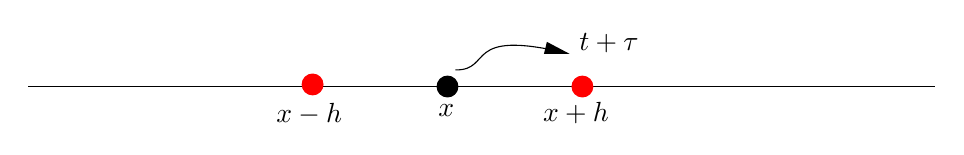
\begin{tikzpicture}[x=0.75pt,y=0.75pt,yscale=-1,xscale=1]
%uncomment if require: \path (0,61); %set diagram left start at 0, and has height of 61

%Straight Lines [id:da8969705158973058] 
\draw [color={rgb, 255:red, 0; green, 0; blue, 0 } ,draw opacity=1 ]   (53,32) -- (250,32) -- (490,32) ;
%Shape: Circle [id:dp7785723770796928] 
\draw  [fill={rgb, 255:red, 0; green, 0; blue, 0 } ,fill opacity=1 ] (250,32) .. controls (250,29.24) and (252.24,27) .. (255,27) .. controls (257.76,27) and (260,29.24) .. (260,32) .. controls (260,34.76) and (257.76,37) .. (255,37) .. controls (252.24,37) and (250,34.76) .. (250,32) -- cycle ;
%Shape: Circle [id:dp7108075326392389] 
\draw  [color={rgb, 255:red, 255; green, 0; blue, 0 } ,draw opacity=1 ][fill={rgb, 255:red, 255; green, 0; blue, 0 } ,fill opacity=1 ] (185,31) .. controls (185,28.24) and (187.24,26) .. (190,26) .. controls (192.76,26) and (195,28.24) .. (195,31) .. controls (195,33.76) and (192.76,36) .. (190,36) .. controls (187.24,36) and (185,33.76) .. (185,31) -- cycle ;
%Shape: Circle [id:dp23106628962253284] 
\draw  [color={rgb, 255:red, 255; green, 0; blue, 0 } ,draw opacity=1 ][fill={rgb, 255:red, 255; green, 0; blue, 0 } ,fill opacity=1 ] (315,32) .. controls (315,29.24) and (317.24,27) .. (320,27) .. controls (322.76,27) and (325,29.24) .. (325,32) .. controls (325,34.76) and (322.76,37) .. (320,37) .. controls (317.24,37) and (315,34.76) .. (315,32) -- cycle ;
%Curve Lines [id:da263551245188425] 
\draw    (258.83,24) .. controls (277.15,24.25) and (262.14,3.91) .. (312.29,15.88) ;
\draw [shift={(313.83,16.25)}, rotate = 193.78] [fill={rgb, 255:red, 0; green, 0; blue, 0 }  ][line width=0.08]  [draw opacity=0] (12,-3) -- (0,0) -- (12,3) -- cycle    ;

% Text Node
\draw (249.33,39.4) node [anchor=north west][inner sep=0.75pt]    {$x$};
% Text Node
\draw (171.33,38.9) node [anchor=north west][inner sep=0.75pt]    {$x-h$};
% Text Node
\draw (299.83,38.4) node [anchor=north west][inner sep=0.75pt]    {$x+h$};
% Text Node
\draw (317.33,5.4) node [anchor=north west][inner sep=0.75pt]    {$t+\tau $};


\end{tikzpicture}

\end{figure}
\FloatBarrier

Usando il teorema delle probabilità totali posso esprimere $\displaystyle p(x,t+\tau)$ in funzione dell'istante precedente
\begin{equation*}
p(x,t+\tau) =\frac{1}{2} p(x-h,t) +\frac{1}{2} p(x+h,t)
\end{equation*}
Passando al limite ottengo $\displaystyle 0=0$, occorre quindi uno sviluppo di Taylor
\begin{gather*}
p(x,t+\tau) =p(x,t) +\tau p_{t}(x,t) +o(\tau)\\
p(x\pm h,t) =p(x,t) \pm hp_{x}(x,t) +\frac{h^{2}}{2} p_{xx}(x,t) +o\left(h^{2}\right)
\end{gather*}
sostituendo nell'equazione
\begin{equation*}
\cancel{p} +\tau p_{t} +o(\tau) =\cancel{\frac{1}{2} p} -\cancel{\frac{1}{2} hp_{x}} +\frac{h^{2}}{4} p_{xx} +\cancel{\frac{1}{2} p} +\cancel{\frac{1}{2} hp_{x}} +\frac{h^{2}}{4} p_{xx} +o\left(h^{2}\right)
\end{equation*}
dividendo per $\displaystyle \tau $ e portando $\displaystyle o(\tau)$ a destra
\begin{equation*}
p_{t} =\frac{1}{2}\frac{h^{2}}{\tau } p_{xx} +o\left(\frac{h^{2}}{\tau }\right) +o(1)
\end{equation*}
Se voglio ottenere una cosa sensata, facendo il limite, il rapporto $\displaystyle h^{2} /\tau $ deve mantenersi finito e positivo (così da mantenere le caratteristiche della passeggiata). Faccio il limite per $\displaystyle h,\tau \rightarrow 0$, assumendo
\begin{equation*}
\frac{h^{2}}{\tau } =2D,\ (D >0)
\end{equation*}
fisso e sotto controllo. Allora $\displaystyle o\left( h^{2} /\tau \right)$ è come se fosse un $\displaystyle o(1)$ visto che $\displaystyle h^{2} /\tau $ è costante. Passando al limite ottengo l'\textbf{equazione di diffusione:}
\begin{equation*}
\boxed{p_{t} =Dp_{xx}}
\end{equation*}
Tornando alla passeggiata aleatoria
\begin{equation*}
\frac{\langle x^{2} \rangle }{t} =2D\ \ \Rightarrow \ \ \sqrt{\langle x^{2} \rangle } =\sqrt{t2D}
\end{equation*}
che significa che, nell'unità di tempo $\displaystyle t=1$, la particella diffonde di una distanza media $\displaystyle \sqrt{2D}$: è questa la caratteristica della passeggiata aleatoria che si conserva passando al limite. Abbiamo dunque dato un significato al coefficiente di diffusione!

Inoltre 
\begin{equation*}
\frac{h}{\tau }\rightarrow \infty 
\end{equation*}
la velocità di spostamento diventa sempre più elevata.
\subsection{Dalla passeggiata aleatoria al moto browniano}

Che cosa è diventata la passeggiata aleatoria? Poniamo $\displaystyle x_{j} =x(jh)$ posizione raggiunta dopo $\displaystyle j$ passi. Introduco la variabile aleatoria
\begin{equation*}
\xi _{j} =\frac{x_{j} -x_{j-1}}{h} =\begin{cases}
1, & p=\frac{1}{2}\\
-1, & p=\frac{1}{2}
\end{cases}
\end{equation*}
Da cui
\begin{equation*}
\langle \xi _{j} \rangle =0,\ \langle \xi ^{2}_{j} \rangle =1
\end{equation*}
Le $\displaystyle \xi _{j}$ sono una famiglia di variabili aleatorie iid. La posizione della particella dopo $\displaystyle N$ passi è 
\begin{equation*}
X_{n} =h\sum ^{N}_{j=1} \xi _{j},\ h=\sqrt{\frac{2Dt}{N}}
\end{equation*}
dove la scelta di $\displaystyle h$ è tale che 
\begin{equation*}
\frac{h^{2}}{\tau } =2D
\end{equation*}
Allora
\begin{equation*}
\ X_{N} =\sqrt{2Dt}\frac{\sum\nolimits ^{N}_{j=1} \xi _{j}}{\sqrt{N}},\ \ \sqrt{N} =\sqrt{\mathrm{Var}\sum ^{N}_{j=1} \xi _{j}}
\end{equation*}
sui cui passando al limite per $\displaystyle N\rightarrow \infty $, grazie al Teorema Centrale Limite ottengo che $\displaystyle X_{N}$ converge in legge ad una normale:
\begin{equation*}
X_{N}\xrightarrow{\mathrm{in\ legge}} N(0,2Dt)
\end{equation*}
che ha come densità proprio la soluzione fondamentale $\displaystyle \Gamma _{D}$.

La passeggiata aleatoria è diventata al limite un moto continuo che, per $\displaystyle D=1/2$, prende il nome di \textbf{moto browniano}.

Di solito si usa la notazione $\displaystyle B(t)$ per indicare la posizione di una particella che si muove di moto Browniano. In realtà al variare del tempo le variabili aleatorie sono definite su uno spazio di probabilità $\displaystyle ( \Omega,\mathcal{F},P)$, con 
\begin{enumerate}
\item $\displaystyle \Omega $ insieme degli eventi elementari
\item $\displaystyle \mathcal{F}$ una $\displaystyle \sigma $-algebra degli eventi misurabili in $\displaystyle \Omega $
\item $\displaystyle P$ un'opportuna misura di probabilità in $\displaystyle \mathcal{F}$
\end{enumerate}

La notazione corretta sarebbe dunque $\displaystyle B(t,\omega),\ \omega \in \Omega $. 
\begin{itemize}
\item Bloccando $\displaystyle t$, otteniamo la variabile aleatoria\begin{equation*}
\omega \longmapsto B(t,\omega) \ 
\end{equation*}
\item Bloccando $\displaystyle \omega $, otteniamo la funzione reale\begin{equation*}
t\longmapsto B(t,\omega)
\end{equation*}

che descrive uno dei possibili cammini di una particella Browniana.
\end{itemize}
\subsection{Passeggiata aleatoria non simmetrica}

Cosa succederebbe se, mantenendo tutte le altre regole uguali, la probabilità che la particella si sposti verso sinistra o verso destra non sia $\displaystyle 1/2$?

Sia $\displaystyle p_{0}$ la probabilità che la particella vada a destra e $\displaystyle q_{0}$ quella che vada a sinistra. Per il teorema delle probabilità totali posso riscrivere l'equazione alle differenze finite
\begin{equation*}
p(x,t+\tau) =p_{0} p(x-h,t) +q_{0} p(x+h,t)
\end{equation*}
sviluppando in serie di Taylor in modo analogo
\begin{align*}
\tau p_{t} +o(\tau) & =p_{0}\left( p-hp_{x} +\frac{h^{2}}{2} p_{xx}\right) +q_{0}\left( p+hp_{x} +\frac{h^{2}}{2} p_{xx}\right) +o\left(h^{2}\right)\\
 & =\underbrace{(p_{0} +q_{0})}_{=1} p+\frac{h^{2}}{2} p_{xx} +(q_{0} -p_{0}) hp_{x} +o\left(h^{2}\right)
\end{align*}
Da cui
\begin{equation*}
p_{t} =\frac{1}{2}\textcolor[rgb]{0.29,0.56,0.89}{\frac{h^{2}}{\tau }} p_{xx} +\textcolor[rgb]{0.96,0.65,0.14}{\frac{(q_{0} -p_{0}) h}{\tau }} p_{x} +o\left(\textcolor[rgb]{0.29,0.56,0.89}{\frac{h^{2}}{\tau }}\right) +o(1)
\end{equation*}
Il termine $\displaystyle \textcolor[rgb]{0.29,0.56,0.89}{\frac{h^{2}}{\tau }}$, come prima, sarà mantenuto costante e lo assumiamo uguale a $\displaystyle 2D$. Questa volta però c'è anche un nuovo termine da tenere sotto controllo:
\begin{equation*}
\textcolor[rgb]{0.96,0.65,0.14}{\frac{(q_{0} -p_{0}) h}{\tau }}=\frac{q_{0} -p_{0}}{h}\textcolor[rgb]{0.29,0.56,0.89}{\frac{h^{2}}{\tau }}
\end{equation*}
Assumiamo dunque 
\begin{equation*}
\lim _{h\rightarrow 0}\frac{q_{0} -p_{0}}{h}=\beta,\ \ \beta \ \text{finito}
\end{equation*}
Passando al limite per $\displaystyle h,\tau \rightarrow 0$ sotto queste ipotesi otteniamo
\begin{equation*}
\boxed{p_{t} =Dp_{xx} +vp_{x}} \ \ v=2\beta D
\end{equation*}
Che cos'è il termine $\displaystyle v$ che abbiamo definito? Le sue dimensioni sono quelle di una velocità
\begin{equation*}
[ v] =LT^{-1} \ \ \ \ v=\lim _{h\rightarrow 0} 2D\frac{q_{0} -p_{0}}{h}
\end{equation*}
$\displaystyle q_{0} -p_{0}$ codifica la tendenza del moto continuo ad andare verso una direzione privilegiata: se $\displaystyle v >0$ il moto tenderà al limite ad andare verso sinistra, se $\displaystyle v< 0$ invece tenderà verso destra. In altre parole, esiste una corrente di intensità $\displaystyle | v| $ che trasporta la particella in una direzione mentre questa diffonde con costante $\displaystyle D$.
\begin{equation*}
p_{t} =\underbrace{Dp_{xx}}_{\mathrm{diffusione}} +\underbrace{vp_{x}}_{ \begin{array}{l}
\mathrm{deriva/drift}\\
\mathrm{trasporto}
\end{array}}
\end{equation*}
La passeggiata aleatoria è diventata un processo di \textbf{diffusione con deriva.}
\section{Inquinante in un canale}

Esaminiamo un semplice modello di trasporto e diffusione: in un canale con corrente che si muove con velocità $\displaystyle v$ costante lungo la direzione positiva dell'asse $\displaystyle x$ è presente un inquinante. L'inquinante galleggia sulla superficie e il canale è molto stretto: possiamo trascurare larghezza e profondità ed approssimarlo ad un modello \textit{unidimensionale}.



\begin{figure}[htpb]
	\centering

\tikzset{every picture/.style={line width=0.75pt}} %set default line width to 0.75pt        

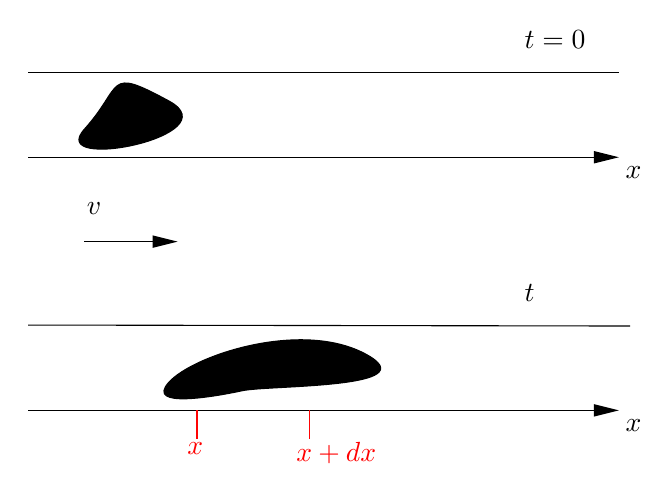
\begin{tikzpicture}[x=0.75pt,y=0.75pt,yscale=-1,xscale=1]
%uncomment if require: \path (0,242); %set diagram left start at 0, and has height of 242

%Straight Lines [id:da44049488951792903] 
\draw    (110,37.1) -- (394.58,37.1) ;
%Shape: Polygon Curved [id:ds6553683057711202] 
\draw  [fill={rgb, 255:red, 0; green, 0; blue, 0 } ,fill opacity=1 ] (177.76,50.65) .. controls (208.62,67.37) and (117.98,85.44) .. (137.1,64.21) .. controls (156.23,42.98) and (146.89,33.94) .. (177.76,50.65) -- cycle ;
%Straight Lines [id:da5485356023961889] 
\draw    (110,77.76) -- (392.58,77.76) ;
\draw [shift={(394.58,77.76)}, rotate = 180] [fill={rgb, 255:red, 0; green, 0; blue, 0 }  ][line width=0.08]  [draw opacity=0] (12,-3) -- (0,0) -- (12,3) -- cycle    ;
%Straight Lines [id:da3109649021932295] 
\draw    (110,158.61) -- (400,159.07) ;
%Shape: Polygon Curved [id:ds8713717377881096] 
\draw  [fill={rgb, 255:red, 0; green, 0; blue, 0 } ,fill opacity=1 ] (272.62,172.62) .. controls (303.48,189.33) and (225.79,187.52) .. (213.19,190.22) .. controls (200.59,192.92) and (166.01,199.22) .. (177.76,186.17) .. controls (189.51,173.12) and (241.75,155.9) .. (272.62,172.62) -- cycle ;
%Straight Lines [id:da4714509137995375] 
\draw    (110,199.72) -- (392.58,199.72) ;
\draw [shift={(394.58,199.72)}, rotate = 180] [fill={rgb, 255:red, 0; green, 0; blue, 0 }  ][line width=0.08]  [draw opacity=0] (12,-3) -- (0,0) -- (12,3) -- cycle    ;
%Straight Lines [id:da9398787311164047] 
\draw    (137.1,118.41) -- (179.96,118.41) ;
\draw [shift={(181.96,118.41)}, rotate = 180] [fill={rgb, 255:red, 0; green, 0; blue, 0 }  ][line width=0.08]  [draw opacity=0] (12,-3) -- (0,0) -- (12,3) -- cycle    ;
%Straight Lines [id:da8968726381584198] 
\draw [color={rgb, 255:red, 255; green, 4; blue, 4 } ,draw opacity=1 ]   (191.31,199.72) -- (191.31,213.27) ;
%Straight Lines [id:da09345282620108719] 
\draw [color={rgb, 255:red, 255; green, 4; blue, 4 } ,draw opacity=1 ]   (245.51,199.72) -- (245.51,213.27) ;

% Text Node
\draw (396.58,81.16) node [anchor=north west][inner sep=0.75pt]  [font=\normalsize]  {$x$};
% Text Node
\draw (347.93,15.6) node [anchor=north west][inner sep=0.75pt]  [font=\normalsize]  {$t=0$};
% Text Node
\draw (396.58,203.12) node [anchor=north west][inner sep=0.75pt]  [font=\normalsize]  {$x$};
% Text Node
\draw (347.93,137.56) node [anchor=north west][inner sep=0.75pt]  [font=\normalsize]  {$t$};
% Text Node
\draw (137,98.4) node [anchor=north west][inner sep=0.75pt]  [font=\normalsize]  {${\textstyle v}$};
% Text Node
\draw (185.37,213.74) node [anchor=north west][inner sep=0.75pt]  [font=\normalsize,color={rgb, 255:red, 255; green, 0; blue, 0 } ,opacity=1 ]  {$x$};
% Text Node
\draw (237.89,213.74) node [anchor=north west][inner sep=0.75pt]  [font=\normalsize,color={rgb, 255:red, 255; green, 0; blue, 0 } ,opacity=1 ]  {$x+dx$};


\end{tikzpicture}

\end{figure}
\FloatBarrier

Vogliamo derivare un modello matematico per descrivere l'evoluzione della concentrazione $\displaystyle c=c(x,t)$ della sostanza. Il tasso di variazione della massa che si trova nell'intervallo $\displaystyle [ x,x+\Delta x]$ è dato da
\begin{equation*}
\frac{d}{dt}\int ^{x+\Delta x}_{x} c(y,t) dy=\int ^{x+\Delta x}_{x} c_{t}(y,t) dy
\end{equation*}
è pari alla differenza tra il flusso in entrata attraverso $\displaystyle x$ e il flusso in uscita attraverso $\displaystyle x+dx$. Indicando con $\displaystyle q=q(x,t)$ il flusso di massa che entra nell'intervallo attraverso il punto $\displaystyle x$ al tempo $\displaystyle t$ posso scrivere la conservazione della massa
\begin{equation*}
\int ^{x+\Delta x}_{x} c_{t}(y,t) dy=q(x,t) -q(x+\Delta x,t)
\end{equation*}
Dividendo per $\displaystyle \Delta x$ e passando al limite per $\displaystyle \Delta x\rightarrow 0$ si ottiene
\begin{equation}
c_{t} =-q_{x}
\label{eq:inquinante-in-canale}
\end{equation}
Ora bisogna decidere con che tipo di flusso di massa abbiamo a che fare o, in altri termini, stabilire una \textbf{legge costitutiva }per $\displaystyle q$:
\begin{itemize}
\item Per \textbf{convezione} o trasporto, il flusso è determinato dalla sola corrente d'acqua, come se l'inquinante fosse trasportato dal fluido senza espandersi o deformarsi\begin{equation*}
q(x,t) =vc(x,t)
\end{equation*}
\item Per \textbf{diffusione}, similmente alla legge di Fourier per il calore, la legge di Fick stabilisce che la diffusione avviene da zone ad alta concentrazione verso zone a bassa concentrazione\begin{equation*}
q(x,t) =-Dc_{x}(x,t)
\end{equation*}
\end{itemize}

Poiché nel nostro caso sono presenti sia trasporto che diffusione, sovrapporremo i due effetti:
\begin{equation*}
q=\text{diffusione} +\text{trasporto} =vc-Dc_{x},\ \ [ q] =MT^{-1}
\end{equation*}
Sostituendo in \eqref{eq:inquinante-in-canale} si trova
\begin{equation*}
\boxed{c_{t} =Dc_{xx} -vc_{x}}
\end{equation*}
\textit{Lezione 8 (15/03/2021)}

Consideriamo un modello del tipo
\begin{equation}
u_{t} =Du_{xx} +bu_{x} +cu
\label{eq:modello-dif-trasp-rea}
\end{equation}
I vari termini rappresentano
\begin{itemize}
\item $Du_{xx}$, \textbf{diffusione}
\item $bu_{x}$, \textbf{trasporto} o deriva (drift) con velocità $v=-b$ nella direzione positiva dell'asse $x$
\item $cu$, \textbf{reazione} ($c >0$, crescita, oppure $c< 0$ decadimento, esponenziale)
\end{itemize}

Qual'è la soluzione fondamentale per \eqref{eq:modello-dif-trasp-rea}, cioè quella soluzione che al tempo iniziale assume distribuzione Dirac in $x=0$?. Si può dimostrare che è
\begin{equation*}
\boxed{\Gamma ^{\star }(x,t) =\frac{1}{\sqrt{4\pi Dt}} e^{ct}\exp\left\{-\frac{(x+bt)^{2}}{4Dt}\right\}}
\end{equation*}
Se $c=0$ abbiamo la solita $\Gamma $ che si trasporta, se $c\gtrless 0$ la $\Gamma $ viene accentuata o smorzata esponenzialmente.

L'equazione generale in $n$ dimensioni è
\begin{equation*}
u_{t} =\mathrm{div}(A(x,t) \nabla u) +\mathrm{div}(\mathbf{b} u) +\mathbf{v} u+cu
\end{equation*}
dove i termini dipendono in questo modo
\begin{equation*}
\mathbf{b} =\mathbf{b}(x,t) \ \ \mathbf{v} =\mathbf{v}(x,t) \ \ c=c(x,t)
\end{equation*}
\section{Problema di Cauchy globale \texorpdfstring{$(n=1)$}{n = 1}}

Consideriamo il problema di Cauchy globale in $n=1$ dimensioni. La generalizzazione a dimensione $n >1$ è standard, quindi lavoriamo in $n=1$ per semplicità.
\begin{equation*}
\text{(PCG)} \ \begin{cases}
u_{t} -Du_{xx} =0 & \text{in} \ \mathbb{R} \times (0,T) \ \ \ \ T\leqslant +\infty \\
u(x,0) =g(x) & \text{in} \ \mathbb{R}
\end{cases}
\end{equation*}
dove $g$ è il \textit{dato iniziale} assegnato.

Interpretiamo $u$ come una \textbf{concentrazione di massa, o densità lineare di massa}, nel senso che $u(x,t) dx$ è la massa che si trova nell'intervallo $(x,x+dx)$ al tempo $t$.

Sappiamo risolvere (PCG) nel caso di impulso nell'origine $g(x) =\delta (x)$ e di conseguenza anche nel caso di $g(x) =\delta (x-y)$.\footnote{Non è corretto usare l'uguaglianza, intendiamo che le distribuzioni hanno lo stesso effetto tramite il prodotto di dualità.} In questa situazione, la soluzione è data da
\begin{equation*}
u(x,t) =\Gamma _{D}(x-y,t)
\end{equation*}
È una \textit{unit-source solution}, nel senso che descrive come si evolve una massa unitaria inizialmente concentrata in $y$. Se avessimo una massa totale di $Q$ anziché unitaria avremmo
\begin{equation*}
u(x,t) =Q\cdotp \Gamma _{D}(x-y,t)
\end{equation*}



\begin{figure}[htpb]
	\centering

\tikzset{every picture/.style={line width=0.75pt}} %set default line width to 0.75pt        

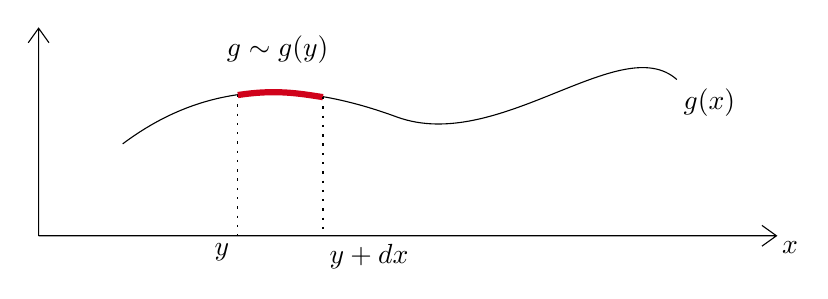
\begin{tikzpicture}[x=0.75pt,y=0.75pt,yscale=-1,xscale=1]
%uncomment if require: \path (0,140); %set diagram left start at 0, and has height of 140

%Shape: Axis 2D [id:dp4931078321995175] 
\draw  (114,110) -- (469.5,110)(114,10) -- (114,110) -- cycle (462.5,105) -- (469.5,110) -- (462.5,115) (109,17) -- (114,10) -- (119,17)  ;
%Curve Lines [id:da7762158719493701] 
\draw    (154.5,65.72) .. controls (194.5,35.72) and (237.5,34.72) .. (286.5,52.72) .. controls (335.5,70.72) and (394.5,10.72) .. (421.5,34.72) ;
%Curve Lines [id:da8187349331902096] 
\draw [color={rgb, 255:red, 208; green, 2; blue, 27 } ,draw opacity=1 ][line width=2.25]    (210,42.2) .. controls (228.2,39.4) and (239.4,41.4) .. (251,43.2) ;
%Straight Lines [id:da9080172774216906] 
\draw  [dash pattern={on 0.84pt off 2.51pt}]  (210,42.2) -- (210,110.4) ;
%Straight Lines [id:da9068454288868981] 
\draw  [dash pattern={on 0.84pt off 2.51pt}]  (251,43.2) -- (251,109.4) ;

% Text Node
\draw (471,111.4) node [anchor=north west][inner sep=0.75pt]    {$x$};
% Text Node
\draw (423.5,38.12) node [anchor=north west][inner sep=0.75pt]    {$g(x)$};
% Text Node
\draw (203.5,12.52) node [anchor=north west][inner sep=0.75pt]    {$g\sim g(y)$};
% Text Node
\draw (197.5,112.52) node [anchor=north west][inner sep=0.75pt]    {$y$};
% Text Node
\draw (253,112.8) node [anchor=north west][inner sep=0.75pt]    {$y+dx$};


\end{tikzpicture}

\end{figure}
\FloatBarrier

La massa presente in $(y,y+dy)$ è $g(y) dy$. L'evoluzione della singola massa $Q=g(y) dy$ è
\begin{equation*}
u(x,t) =\Gamma _{D}(x-y,t) g(y) dy
\end{equation*}
Per il principio di sovrapposizione possiamo sommare tutti i contributi
\begin{equation*}
u(x,t) =\int _{\mathbb{R}} \Gamma _{D}(x-y,t) g(y) dy
\end{equation*}
che è una \textbf{convoluzione} del dato iniziale con la gaussiana
\begin{equation*}
u(x,t) =( \Gamma _{D}(\cdotp,t) *g)(x)
\end{equation*}
è la \textit{candidata} soluzione di (PCG).
\subsection{Esistenza}

\textbf{Problemi.}
\begin{enumerate}
\item L'integrale è ben definito? Se $g(x) \sim e^{m| x| },m >2$ per $| x| \rightarrow +\infty $, la gaussiana compensa potenze fino al $2$, quindi ci si aspetta che l'integrale non converga! Non posso scegliere $g$ come voglio, ma dovrò dare delle opportune condizioni all'infinito.
\item Supponiamo che converga, è vero che $u$ è soluzione dell'equazione differenziale? In altre parole posso passare sotto il segno di integrale?
\item Supponiamo che sia soluzione, in che senso $u(x,0) =g(x)$?
\item Se tutto sopra va bene, $u$ è anche l'unica?
\end{enumerate}

Si trova risposta all'esistenza nel seguente fondamentale teorema, dalla dimostrazione piuttosto lunga, che omettiamo.
\begin{theorem}
[di Esistenza] Sia $g$ una funzione con un numero \textbf{finito} di punti di \textbf{discontinuità} e tale che $\exists c,a$ che la limitano secondo
\begin{equation}
| g(x)| \leqslant ce^{ax^{2}} \ \ \forall x\in \mathbb{R} \tag{G}
\end{equation}
Sia
\begin{equation*}
u(x,t) =\int _{\mathbb{R}} \Gamma _{D}(x-y,t) g(y) dy
\end{equation*}
Allora
\begin{enumerate}
\item $u$ è ben definita e di classe $C^{\infty }$ in ogni strisica del tipo $\mathbb{R} \times (0,T)$, con $T< \frac{1}{4aD}$ e inoltre in tale striscia $u_{t} -Du_{xx} =0$.
\item Se $x_{0}$ è un punto di continuità per $g$, allora\begin{equation*}
u(x,t)\rightarrow g(x_{0}) \ \ \text{se} \ (x,t)\rightarrow (x_{0},0)
\end{equation*}

In particolare se $g\in C(\mathbb{R})$, allora $u\in C(\mathbb{R} \times [ 0,T])$, \textbf{chiuso} a sinistra.
\item Esistono due costanti $C,A$ tali che\begin{equation*}
| u(x,t)| \leqslant Ce^{Ax^{2}} \ \ \forall (x,t) \in \mathbb{R} \times [ 0,T]
\end{equation*}
\end{enumerate}
\end{theorem}

Questo risponde a $1,2,3$. Occupiamoci dell'unicità.
\begin{oss}
In molti casi il dato iniziale $g$ è polinomiale, e il teorema è quindi soddisfatto per ogni scelta di $a$ e $c$, in particolare ci permette di estendere l'invervallo temporale quanto vogliamo esse $T< \frac{1}{4Da}$, con $a$ arbitrariamente piccolo.
\end{oss}
\begin{oss}
[Processo regolarizzante] Il primo enunciato sottolinea che anche se il dato iniziale è discontinuo da qualche parte (può esserlo in un numero finito di punti), subito dopo il primo istante la soluzione diventa continua e $C^{\infty }$.
\end{oss}
Per il dato iniziale
\begin{equation*}
g(x) =\chi _{(-2,0)}(x) +\chi _{(1,4)}(x)
\end{equation*}

\fg{0.7}{diffusione-effetto-regolarizzante}

\begin{oss}
Se $g$ è limitata (cioè $a=0$ in (G)) allora $u$ è definita in $\mathbb{R} \times (0,+\infty)$.
\end{oss}
\subsection{Unicità}

In generale non c'è unicità, vediamo il controesempio di Tychonov
\begin{equation*}
h(t) =\begin{cases}
e^{-t^{-2}}, & t >0\\
0, & t\leqslant 0
\end{cases} \ \ \text{cioè tale che} \ h^{(k)}(t)\xrightarrow{t\rightarrow 0} 0,\ \forall k=0,1,2\dotsc 
\end{equation*}
La funzione costruita come
\begin{equation*}
\Tau (x,t) =\sum\limits ^{\infty }_{k=0}\frac{h^{(k)}(t)}{(2k) !} x^{2k}
\end{equation*}
è soluzione dell'equazione $\Tau _{t} -\Tau _{xx} =0,\ \Tau (x,0) =0$ assunto con continuità.

Si dimostra per induzione che $\exists \vartheta  >0$ tale che $\forall t >0$
\begin{equation*}
\left| h^{(k)}(t)\right| \leqslant \frac{k!}{(\vartheta t)^{k}}\exp\left( -\frac{1}{2} t^{-2}\right)
\end{equation*}
è chiaro che
\begin{equation*}
| \Tau (x,t)| \leqslant \sum\limits ^{\infty }_{k=0}\underbrace{\frac{k!}{(2k) !}}_{< \frac{1}{k!}}\frac{x^{2k}}{(\vartheta t)^{k}}\exp\left( -\frac{1}{2} t^{-2}\right) \leqslant \exp\left(\frac{x^{2}}{\vartheta t} -\frac{1}{2t^{2}}\right)
\end{equation*}
avendo riconosciuto la serie dell'esponenziale. Per $x$ fissato e $t\rightarrow 0$, allora $| \Tau (x,t)| \rightarrow 0$.

Si verifica che
\begin{equation*}
\Tau _{t}(x,t) =\sum\limits ^{\infty }_{k=0}\frac{h^{(k+1)}(t)}{(2k) !} x^{2k} =\sum\limits ^{\infty }_{k=2}\frac{h^{(k)}(t)}{(2k-2) !} x^{2k-2} =\Tau _{xx}(x,t)
\end{equation*}
quindi $\Tau (x,t)$ rispetta l'equazione differenziale e anche il teorema di esistenza. Tuttavia anche la soluzione identicamente nulla è, ovviamente, soluzione del problema. Segue che \textbf{in generale la soluzione non è unica}. Il problema è che $\Tau $ cresce troppo quando $x\rightarrow \pm \infty $ per tempi $t$ piccoli a causa del termine
\begin{equation*}
\frac{x^{2}}{\vartheta t}
\end{equation*}
Se al posto di $\vartheta t$ ci fosse una costante andrebbe meglio: si definisce una classe di soluzioni a crescita controllata che garantisce l'unicità.
\begin{definition}
[Classe di Tychonov]
\begin{equation*}
| u(x,t)| \leqslant Ce^{Ax^{2}},\ \ \forall x\in \mathbb{R},t\in [ 0,T]
\end{equation*}
\end{definition}
\begin{theorem}
[Principio di massimo globale] Sia $u\in C(\mathbb{R} \times [ 0,T])$, con $u_{t},u_{x},u_{xx}$ continue in $\mathbb{R} \times (0,T)$, tale che in $\mathbb{R} \times (0,T)$
\begin{enumerate}
\item Sia una sottosoluzione dell'equazione del calore\begin{equation*}
u_{t} -Du_{xx} \leqslant 0\ \ \ \ (\geqslant)
\end{equation*}
\item Sia dominata da un esponenziale, $C >0$\begin{equation*}
u(x,t) \leqslant Ce^{Ax^{2}} \ \ \ \ \left( \geqslant -Ce^{Ax^{2}}\right)
\end{equation*}
\end{enumerate}
Allora
\begin{equation*}
\sup _{\mathbb{R} \times [ 0,T]} u(x,t) \leqslant \sup _{\mathbb{R}} u(x,0) \ \ \ \ (\inf_{\mathbb{R} \times [ 0,T]} u(x,t) \geqslant \inf_{\mathbb{R}} u(x,0))
\end{equation*}
\end{theorem}

Se $u$ fosse soluzione dell'equazione
\begin{equation*}
\begin{cases}
u_{t} -Du_{xx} =0 & \text{in} \ \mathbb{R} \times (0,T)\\
u\ \text{nella classe di Tychonov} & 
\end{cases}
\end{equation*}
allora
\begin{equation*}
u(x,0) =0\ \ \text{implica} \ \ u(x,t) =0\ \ \text{in} \ \mathbb{R} \times [ 0,T]
\end{equation*}
\textbf{Conseguenza.}

La
\begin{equation*}
u(x,t) =\int _{\mathbb{R}} \Gamma _{D}(x-y,t) g(y) dy
\end{equation*}
definita nel teorema di Esistenza è unica all'interno della Classe di Tychonov, che era comunque richiesta in tale teorema al punto $3$, pertanto fornisce non solo esistenza, ma anche unicità!
\chapter{Equazione di Laplace-Poisson}
\begin{definition}
[Equazione di Poisson] Si definisce
\begin{equation*}
\boxed{-\Delta u=f} \ \ \text{in} \ \Omega \ \text{dominio limitato in} \ \mathbb{R}^{n}
\end{equation*}
\end{definition}
da dove viene fuori?
\begin{itemize}
\item Temperatura a regime stazionario con $D=1$ dell'equazione del calore.
\item $\mathbf{E}$ campo elettrostatico generato da una distribuzione di carica $\rho $ in $\Omega \subset \mathbb{R}^{3}$ in unità $Mks$:\begin{equation*}
\mathrm{div}\mathbf{E} =\frac{4\pi \rho }{\varepsilon }
\end{equation*}

$\varepsilon $ costante dielettrica.

Se il campo è conservativo esiste uno scalare $u$, potenziale elettrostatico, tale che $\nabla u=-\mathbf{E}$ allora\begin{equation*}
\mathrm{div}\mathbf{E} =-\mathrm{div}(\nabla u) =-\Delta u=\frac{4\pi \rho }{\varepsilon }
\end{equation*}

In assenza di cariche $\rho =0$ e quindi il potenziale è armonico $\Delta u=0$.
\item Le parti reali e immaginarie di una funzione olomorfa sono armoniche. Poiché per esempio le funzioni al variare di $m\in \mathbb{N}$

\begin{equation*}
z^{m} =\rho ^{m}(\cos m\vartheta +i\sin m\vartheta)
\end{equation*}

sono olomorfe in $\mathbb{C}$, di conseguenza le funzioni

\begin{equation*}
\begin{cases}
u( \rho,\vartheta) =\rho ^{m}\cos m\vartheta \\
v( \rho,\vartheta) =\rho ^{m}\sin m\vartheta 
\end{cases}
\end{equation*}

sono armoniche. Tra esse per esempio\begin{equation*}
m=2,\ \ z^{2} =\left( x^{2} -y^{2}\right) +ixy\ \ \Rightarrow \ \ \begin{cases}
u=x^{2} -y^{2}\\
v=xy
\end{cases}
\end{equation*}
\end{itemize}
\section{Tipici problemi al bordo}

Sono le condizioni che troviamo nell'equazione del calore nella parte laterale
\begin{itemize}
\item \textbf{Dirichlet} $u=g$ su $\partial \Omega $
\item \textbf{Neumann} $\partial _{\nu } u=h$ su $\partial \Omega $
\item \textbf{Robin} $\partial _{\nu } u+\alpha u=h$, con $\alpha  >0$
\item miste
\end{itemize}
\textit{Lezione 9 (16/03/2021)}

\begin{theorem}
	Sia $\displaystyle \Omega \subset \mathbb{R}^{n}$ un dominio limitato regolare. Allora esiste al più una funzione $\displaystyle u$ di classe $\displaystyle C^{2}(\Omega) \cap C^{1}(\overline{\Omega })$ soluzione di $\displaystyle \Delta u=f$ in $\displaystyle \Omega $ con condizioni di Dirichlet o Robin. Nel caso di Neumann, due soluzioni differiscono per una costante.
\end{theorem}
\begin{dimostrazione}
	Siano $\displaystyle u$ e $\displaystyle v$ soluzioni di uno dei problemi indicati con lo stesso dato al bordo $\displaystyle g$. Sia $\displaystyle w=u-v$, allora $\displaystyle w$ è armonica in $\displaystyle \Omega $
	\begin{equation*}
		\Delta w=\Delta u-\Delta v=-f+f=0
	\end{equation*}
	con dato al bordo $\displaystyle g=0$. Moltiplicando per $\displaystyle w$ e integrando su $\displaystyle \Omega $
	\begin{equation*}
		\int _{\Omega } w\Delta w=0
	\end{equation*}
	Da cui, utilizzando l'identità di Green \eqref{eq:id-green}
	\begin{equation*}
		-\int _{\Omega }| \nabla w| ^{2} +\int _{\partial \Omega } w\partial _{\nu } w\ d\sigma =0\ \ \Rightarrow \ \ \int _{\Omega }| \nabla w| ^{2} =\int _{\partial \Omega } w\partial _{\nu } w\ d\sigma 
	\end{equation*}
	Ora analizziamo nello specifico i tre possibili casi:
	\begin{itemize}
		\item \textbf{Dirichlet}
		      
		      Essendo $\displaystyle w=0$ su $\displaystyle \partial \Omega $ si trova
		      
		      \begin{align*}
		      	\int _{\Omega }| \nabla w| ^{2} =0\ \&\Rightarrow \ \ \nabla w=0\ \text{in} \ \mathrm{\Omega } &                                                          \\
		      	                                      & \Rightarrow \ \ w=\text{cost. in} \ \Omega               
		      \end{align*}
		      
		      Ma dato che $\displaystyle w=0$ su $\displaystyle \partial \Omega $, la costante deve essere $\displaystyle 0$, da cui $\displaystyle w\equiv 0$.
		\item \textbf{Robin}
		      
		      Essendo $\displaystyle \partial _{\nu } w=-\alpha w$
		      
		      \begin{align*}
		      	\int _{\Omega }| \nabla w| ^{2} =-\alpha \int _{\partial \Omega } w^{2} d\sigma & \leqslant 0                                    \\
		      	                                                                                & \Rightarrow \ \ \nabla w=0\ \text{in} \ \Omega \\
		      	                                                                                & \Rightarrow \ \ w=\text{cost. in} \ \Omega     
		      \end{align*}
		      
		      ma allora $\displaystyle w=0$ su $\displaystyle \partial \Omega \Rightarrow w\equiv 0$ in $\displaystyle \Omega $.
		\item \textbf{Neumann}
		      
		      Essendo $\displaystyle \partial _{\nu } w=0$
		      
		      \begin{equation*}
		      	\int _{\Omega }| \nabla w| ^{2} =0\ \ \Rightarrow \ \ w=\text{cost. in} \ \Omega 
		      \end{equation*}
		      
		      Non posso fare alcuna affermazione aggiuntiva.
	\end{itemize}
\end{dimostrazione}
Nel caso Neumann non vale l'unicità, ma in generale non vale neanche l'esistenza, infatti da 
\begin{equation*}
	-\Delta u=f,\ \partial _{\nu } u=g\ \text{su} \ \partial \Omega 
\end{equation*}
integrando su $\displaystyle \Omega $ si trova
\begin{equation*}
	-\int _{\Omega } \Delta u=\int _{\Omega } f
\end{equation*}
e applicando il teorema di Gauss \eqref{eq:id-green-v1}
\begin{equation*}
	\Rightarrow \ \ -\int _{\partial \Omega } \partial _{\nu } ud\sigma =\int _{\Omega } f\ \ \Rightarrow \ \ \boxed{\int _{\Omega } f+\int _{\partial \Omega } gd\sigma =0}
\end{equation*}
Abbiamo trovato una condizione necessaria per la risolubilità del problema di Neumann. Per esempio:
\begin{equation*}
	\begin{cases}
		-\Delta u=1          & \text{in} \ \Omega \\
		\partial _{\nu } u=0 &                    
	\end{cases}
\end{equation*}
non ha soluzione! La condizione necessaria che abbiamo trovato infatti darebbe
\begin{equation*}
	\int _{\Omega } 1=0
\end{equation*}
\section{Funzioni armoniche nel discreto}

Per esaminare le proprietà delle funzioni armoniche torniamo ad esplorare il legame tra modelli discreti e continui, probabilistici e deterministici. Ritorniamo alla passeggiata aleatoria, lavorando questa volta in dimensione $\displaystyle n=2$. Allora detti $\displaystyle h >0$ passo spaziale, e $\displaystyle \tau  >0$ passo temporale, introduciamo $\displaystyle h\mathbb{Z}^{2}$ il reticolo dei punti 
\begin{equation*}
	\begin{cases}
		x=(x_{1},x_{2}) &                 \\
		x_{1} =mh         & m\in \mathbb{Z} \\
		x_{2} =nh         & n\in \mathbb{Z} 
	\end{cases}
\end{equation*}
La particella si muove in ciascuna delle quattro direzioni con probabilità identica $\displaystyle 1/4$, e i versori degli assi $\displaystyle x_{1},x_{2}$ sono rispettivamente $\displaystyle \vec{e}_{1},\vec{e}_{2}$.

Sia $\displaystyle p(x,t) =p(x_{1},x_{2},t)$ la probabilità di trovare la particella nel punto $\displaystyle x$ al tempo $\displaystyle t$. Come nella precedente passeggiata cerchiamo di ricavare un'equazione alle differenze per $\displaystyle p$ col teorema delle probabilità totali.
\begin{equation*}
	p( x_{1},x_{2},t+\tau) =\frac{1}{4}\{p( x-h\vec{e}_{1},t) +p( x+h\vec{e}_{1},t) +p( x-h\vec{e}_{2},t) +p( x+h\vec{e}_{2},t)\}
\end{equation*}
Quella che troviamo è esattamente la media aritmetica dei valori di $\displaystyle p(\cdotp,t)$ nei punti dell'intorno discreto di $\displaystyle x$ di raggio $\displaystyle h$. 

Trascurando per ora il tempo, definisco l'operatore di media su una generica funzione $\displaystyle u=u(x),\ x\in h\mathbb{Z}^{2}$
\begin{equation*}
	M_{h} u(x) =\frac{1}{4}\sum _{| x-y| =h} u(y)
\end{equation*}
In questo modo posso riscrivere l'equazione alle differenze sfruttando l'operatore
\begin{equation*}
	p( x_{1},x_{2},t+\tau) =M_{h} p(x,t)
\end{equation*}
Sviluppando fino al secondo ordino con Taylor
\begin{gather*}
	M_{h} u(x) =\frac{1}{4}\left\{4u(x) +\underbrace{h^{2} u_{x_{1} x_{1}}(x) +h^{2} u_{x_{2} x_{2}}(x)}_{h^{2} \Delta u(x)}\right\} +o\left(h^{2}\right)\\
	\Rightarrow \ \ \lim _{h\rightarrow 0}\frac{M_{h} u(x) -u(x)}{h^{2}} =\frac{1}{4} \Delta u(x)
\end{gather*}
In base a questo risultato è coerente definire il laplaciano discreto
\begin{equation}
	\Delta ^{*}_{h} u(x) =\frac{4}{h^{2}}(M_{h} u(x) -u(x))
\end{equation}
Se $\displaystyle \Delta ^{*}_{h} u=0$ (ovvero se in ogni punto $\displaystyle x$ la funzione coincide con la media dei propri valori nei punti dell'intorno discreto di $\displaystyle x$ di raggio $\displaystyle h$) la funzione verrà chiamata \textbf{d-armonica} (dove d sta per discreto).

Cerchiamo ora di definire il problema di Dirichlet discreto nel reticolo: per farlo servono prima delle nozioni di topologia discreta.

Sia $\displaystyle A\in h\mathbb{Z}^{2}$. Diciamo che $\displaystyle x\in A$ è
\begin{itemize}
	\item \textbf{interno} ad $\displaystyle A$ se il suo intorno discreto di raggio $\displaystyle h$ è contenuto in $\displaystyle A$;
	\item \textbf{punto di frontiera} se non è interno ad $\displaystyle A$ ma il suo intorno discreto di raggio $\displaystyle h$ contiene almeno un punto interno;
	\item \textbf{isolato} se non è interno o di frontiera.
\end{itemize}

$\displaystyle A$ è detto \textbf{connesso} se non ha punti isolati e $\displaystyle \forall x_{0},x_{1} \in A\ x_{0},x_{1}$ possono essere collegati da un cammino discreto contenuto interamente in $\displaystyle A$

\fg[Esempio di dominio connesso di $\displaystyle h\mathbb{Z}^{2}$]{0.4}{laplace-dominio-connesso-discreto}

\textbf{Problema di Dirichlet discreto}: sia $\displaystyle A$ dominio limitato e connesso di $\displaystyle h\mathbb{Z}^{2}$, sia $\displaystyle g$ definita su $\displaystyle \partial A$. Determinare $\displaystyle u$, definito su $\displaystyle A$, tale che
\begin{equation}
	\begin{cases}
		\Delta ^{*}_{h} u=0 & \text{nei punti interni ad} \ A \\
		u=g                 & \text{su} \ \partial A          
	\end{cases}
	\label{eq:pb-dirichlet-discreto}
\end{equation}
Proprietà di una soluzione di \eqref{eq:pb-dirichlet-discreto}:
\begin{enumerate}
	\item \textbf{Principio di massimo}. Se $\displaystyle u$ assume massimo o minimo in un punto interno ad $\displaystyle A$, allora $\displaystyle u$ è costante. Infatti
		\begin{figure}[htpb]
	      	\centering
	      	

	      	\tikzset{every picture/.style={line width=0.75pt}} %set default line width to 0.75pt        

	      	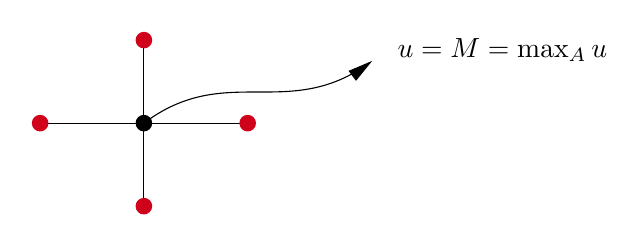
\begin{tikzpicture}[x=0.75pt,y=0.75pt,yscale=-1,xscale=1]
	      	%uncomment if require: \path (0,106); %set diagram left start at 0, and has height of 106

	      	%Straight Lines [id:da019234409051198664] 
	      	\draw    (99,54.5) -- (199,54.5) ;
	      	%Straight Lines [id:da2169607633909847] 
	      	\draw    (149,14.5) -- (149,94.5) ;
	      	%Shape: Ellipse [id:dp036734699586719044] 
	      	\draw  [draw opacity=0][fill={rgb, 255:red, 208; green, 2; blue, 27 }  ,fill opacity=1 ][line width=3]  (145,14.5) .. controls (145,12.29) and (146.79,10.5) .. (149,10.5) .. controls (151.21,10.5) and (153,12.29) .. (153,14.5) .. controls (153,16.71) and (151.21,18.5) .. (149,18.5) .. controls (146.79,18.5) and (145,16.71) .. (145,14.5) -- cycle ;
	      	%Shape: Ellipse [id:dp594871404717175] 
	      	\draw  [draw opacity=0][fill={rgb, 255:red, 0; green, 0; blue, 0 }  ,fill opacity=1 ][line width=3]  (145,54.5) .. controls (145,52.29) and (146.79,50.5) .. (149,50.5) .. controls (151.21,50.5) and (153,52.29) .. (153,54.5) .. controls (153,56.71) and (151.21,58.5) .. (149,58.5) .. controls (146.79,58.5) and (145,56.71) .. (145,54.5) -- cycle ;
	      	%Curve Lines [id:da06865790719302067] 
	      	\draw    (149,54.5) .. controls (188.6,24.8) and (218.4,53.91) .. (257.8,25.38) ;
	      	\draw [shift={(259,24.5)}, rotate = 503.13] [fill={rgb, 255:red, 0; green, 0; blue, 0 }  ][line width=0.08]  [draw opacity=0] (12,-3) -- (0,0) -- (12,3) -- cycle    ;
	      	%Shape: Ellipse [id:dp4253248089812065] 
	      	\draw  [draw opacity=0][fill={rgb, 255:red, 208; green, 2; blue, 27 }  ,fill opacity=1 ][line width=3]  (195,54.5) .. controls (195,52.29) and (196.79,50.5) .. (199,50.5) .. controls (201.21,50.5) and (203,52.29) .. (203,54.5) .. controls (203,56.71) and (201.21,58.5) .. (199,58.5) .. controls (196.79,58.5) and (195,56.71) .. (195,54.5) -- cycle ;
	      	%Shape: Ellipse [id:dp674183510238525] 
	      	\draw  [draw opacity=0][fill={rgb, 255:red, 208; green, 2; blue, 27 }  ,fill opacity=1 ][line width=3]  (145,94.5) .. controls (145,92.29) and (146.79,90.5) .. (149,90.5) .. controls (151.21,90.5) and (153,92.29) .. (153,94.5) .. controls (153,96.71) and (151.21,98.5) .. (149,98.5) .. controls (146.79,98.5) and (145,96.71) .. (145,94.5) -- cycle ;
	      	%Shape: Ellipse [id:dp7646484647440714] 
	      	\draw  [draw opacity=0][fill={rgb, 255:red, 208; green, 2; blue, 27 }  ,fill opacity=1 ][line width=3]  (95,54.5) .. controls (95,52.29) and (96.79,50.5) .. (99,50.5) .. controls (101.21,50.5) and (103,52.29) .. (103,54.5) .. controls (103,56.71) and (101.21,58.5) .. (99,58.5) .. controls (96.79,58.5) and (95,56.71) .. (95,54.5) -- cycle ;

	      	% Text Node
	      	\draw (270,12.4) node [anchor=north west][inner sep=0.75pt]    {$u=M=\max_{A} u$};


	      	\end{tikzpicture}
		\end{figure}
		\FloatBarrier
		$\displaystyle \Rightarrow u=M$ nei punti del suo intorno discreto (visto che il punto centrale è la media dei 4 punti, tutti devono essere punti di massimo). Reiterando il ragionamento per ogni altro punto dell'intorno posso propagarlo fino alla frontiera.
	\item $\displaystyle u$ assume max e min su $\displaystyle \partial A$ (immediata conseguenza del punto 1)
	\item La soluzione di \eqref{eq:pb-dirichlet-discreto} è unica
\end{enumerate}
Posso risolvere il problema di Dirichlet discreto con metodi probabilistici, tornando alla passeggiata aleatoria. 

Interpretiamo $\displaystyle g$ come una sorta di \textbf{guadagno}: se la particella parte da $\displaystyle x$ e raggiunge la frontiera di $\displaystyle A$ per la prima volta in $\displaystyle y$ otteniamo un guadagno $\displaystyle g(y)$. Voglio dimostrare che, qualunque sia il punto di partenza $\displaystyle x$, la particella raggiunge $\displaystyle \partial A$ con probabilità $\displaystyle 1$ e che il valore di $\displaystyle u(x)$, la soluzione che vogliamo costruire, è il valore atteso del guadagno $\displaystyle g$ rispetto ad un'opportuna distribuzione di probabilità su $\displaystyle \partial A$. 

Indichiamo con $\displaystyle \Gamma $ un qualunque sottoinsieme di $\displaystyle \partial A$ e con $\displaystyle P(x,\Gamma)$ la probabilità che la particella che parte da $\displaystyle x$ raggiunga per la prima volta la $\displaystyle \partial A$ in un punto $\displaystyle y\in \Gamma $. 

Dobbiamo dimostrare che $\displaystyle P(x,\partial A) =1\ \forall x\in A$. Indico con $\displaystyle w_{\Gamma }(x)$ la funzione che ottengo al variare di $\displaystyle x$ in $\displaystyle P(x,\Gamma)$ con $\displaystyle \Gamma $ fissato:
\begin{equation*}
	x\longmapsto w_{\Gamma }(x) \equiv P(x,\Gamma),\ \Gamma \ \text{fissato}
\end{equation*}
Facciamo vedere che è d-armonica nei punti interni ad $\displaystyle A$, cioè che $\displaystyle \Delta ^{*}_{h} w_{\Gamma } =0$. Usando il teorema delle probabilità totali
\begin{equation*}
	w_{\Gamma }(x) =P(x,\Gamma) =\frac{1}{4}\sum _{| x-y| =h} P(y,\Gamma) =\frac{1}{4}\sum _{| x-y| =h} w_{\Gamma }(y) =M_{h} w_{\Gamma }(x)
\end{equation*}
Da cui
\begin{gather*}
	M_{h} w_{\Gamma }(x) -w_{\Gamma }(x) =0\\
	\Rightarrow \ \ \Delta ^{*}_{h} w_{\Gamma } =\frac{4}{h^{2}}( M_{h} w_{\Gamma }(x) -w_{\Gamma }(x)) =0
\end{gather*}
in tutti i punti interni ad $\displaystyle A$! 

E invece sulla $\displaystyle \partial A$? Ovviamente se 
\begin{align*}
	x\in \Gamma                       & \ \ \Rightarrow \ \ P(x,\Gamma) =1 \\
	x\in \partial \Gamma \backslash A & \ \ \Rightarrow \ \ P(x,\Gamma) =0 
\end{align*}
Quindi
\begin{equation*}
	w_{\Gamma }(x) =\begin{cases}
	1 & x\in \Gamma \\
	0 & x\in \partial A\backslash \Gamma 
	\end{cases}
\end{equation*}
Ma allora prendendo $\displaystyle \Gamma =\partial A$, $\displaystyle w_{\partial A}(x) =P(x,\partial A)$ è soluzione del problema di Dirichlet discreto con valore 1 sul bordo ($\displaystyle g\equiv 1)$
\begin{equation*}
	\begin{cases}
		\Delta ^{*}_{h} w_{\Gamma }(x) =0 & x\ \text{interno ad} \ A \\
		w_{\partial A}(x) =1              & x\in \partial A          
	\end{cases}
\end{equation*}
Ma anche la funzione $\displaystyle z(x) \equiv 1$ è d-armonica, con gli stessi valori al bordo e soluzione dello stesso problema di Dirichlet. Poiché per la terza proprietà, la soluzione è unica 
\begin{gather*}
	w_{\partial A}(x) =z(x) \equiv 1\ \forall x\in A\\
	\Rightarrow \ \ w_{\partial A}(x) =P(x,\partial A) =1\ \forall x\in A
\end{gather*}
La probabilità di raggiungere la frontiera di $\displaystyle A$ partendo da un qualunque punto interno di $\displaystyle A$ è uguale a $\displaystyle 1$. Se invece prendiamo la funzione
\begin{equation*}
	\Gamma \longmapsto P(x,\Gamma),\ x\ \text{fissato}
\end{equation*}
con $\displaystyle P(x,\partial A) =1$, prendendo $\displaystyle \Gamma _{1},\Gamma _{2} \subset A$, $\displaystyle \Gamma _{1} \cap \Gamma _{2} =\emptyset $
\begin{equation*}
	P( x,\Gamma _{1} \cup \Gamma _{2}) =P(x,\Gamma _{1}) +P(x,\Gamma _{2})
\end{equation*}
è additiva e definisce dunque una misura di probabilità su $\displaystyle \partial A$, $\displaystyle \forall x\in A$ fissato. Fatti tutti questi passaggi possiamo ora costruire la soluzione $\displaystyle u$.
\begin{theorem}
	Il valore della soluzione $\displaystyle u$ in $\displaystyle x\in A$ è il valore atteso dei guadagni $\displaystyle g(y)$ rispetto alla distribuzione di probabilità $\displaystyle P(x,\Gamma)$ cioè
	\begin{equation*}
		u(x) =\sum _{y\in \partial A} g(y) P(x,\{y\})
	\end{equation*}
\end{theorem}
\begin{dimostrazione}
	$\displaystyle u$ è d-armonica, essendolo $\displaystyle x\longmapsto P(x,\{y\})$: ogni addendo
	\begin{equation*}
		g(y) P(x,\{y\}) =g(y) w_{\{y\}}(x)
	\end{equation*}
	è d-armonico in $\displaystyle A$. Inoltre se $\displaystyle z\in \partial A$ allora $\displaystyle u(z) =g(z)$ poiché
	\begin{equation*}
		u(z) =\sum _{y\in \partial A} g(y) P(z,\{y\})
	\end{equation*}
	ed ogni termine nella somma è uguale a $\displaystyle g(z)$ se $\displaystyle y=z$ oppure a zero se $\displaystyle y\neq z$, infatti
	\begin{equation*}
		\begin{cases}
			P(z,\{y\}) =1 & z=y,\ z\in \partial A     \\
			P(z,\{y\}) =0 & z\neq y,\ z\in \partial A 
		\end{cases}
	\end{equation*}
\end{dimostrazione}
\section{Funzioni armoniche}

Sia $\displaystyle \Omega \subseteq \mathbb{R}^{n}$ un dominio, $\displaystyle u$ è armonica in $\displaystyle \Omega $ se $\displaystyle u\in C^{2}(\Omega)$ e $\displaystyle \Delta u=0$ in $\displaystyle \Omega $. 

Quando il passo spaziale $\displaystyle h\rightarrow 0$ le funzioni d-armoniche "diventano" armoniche: è ragionevole che versioni appropriate delle proprietà per funzioni d-armoniche continuino a valere nel caso continuo. La prima è la proprietà di media.
\subsection{Proprietà di media}

Le funzioni d-armoniche sono definite in termini di proprietà di media, quindi ci aspettiamo che le funzioni armoniche ereditino una proprietà di media del tipo: il valore al centro di ogni sfera $\displaystyle B_{R}(x) \subset \subset \Omega $\footnote{Questa notazione è equivalente a $\displaystyle \overline{B_{R}}(x) \subset \Omega $, indica che la supeficie della sfera non tocca la frontiera di $\displaystyle \Omega $ } è uguale alla media artimetica dei valori al bordo della sfera $\displaystyle \partial B_{R}$.

Indichiamo con $\displaystyle \omega _{n}$ la misura di $\displaystyle \partial B_{1}$, la superficie della sfera in $\displaystyle n$ dimensioni di raggio $\displaystyle 1$. Quindi $\displaystyle w_{n} =| \partial B_{1}| $:
\begin{align*}
	w_{2} & =2\pi                                                   \\
	w_{3} & =4\pi                                                   \\
	w_{n} & =\frac{n\pi ^{n/2}}{\Gamma \left(\frac{n}{2} +1\right)} 
\end{align*}
Dove la funzione Gamma di Eulero è definita come
\begin{equation*}
	\Gamma (s) =\int ^{+\infty }_{0} t^{s-1} e^{-t} dt
\end{equation*}
\begin{theorem}
	Sia $\displaystyle u$ armonica in $\displaystyle \Omega \subseteq \mathbb{R}^{n}$. $\displaystyle \forall $ sfera $\displaystyle B_{R}(x) \subset \subset \Omega $ valgono le seguenti formule:\footnote{Nota che $\displaystyle w_{n} R^{n-1}$ è la misura $\displaystyle | \partial B_{R}(x)| $, mentre $\displaystyle \frac{w_{n} R^{n}}{n}$ è semplicemente la misura $\displaystyle | B_{R}(x)| $. I due coefficienti moltiplicativi nelle formule non fanno altro che riscalare rispettivamente per la misura della superficie della sfera e per la misura della sfera stessa: da questo deriva l'interpretazione di "proprietà di media".}
	\begin{equation}
		u(x) =\frac{1}{w_{n} R^{n-1}}\int _{\partial B_{R}(x)} u(\sigma) d\sigma 
		\label{eq:lap-prop-media-i}
	\end{equation}
	\begin{equation}
		u(x) =\frac{n}{w_{n} R^{n}}\int _{B_{R}(x)} u(y) dy
		\label{eq:lap-prop-media-ii}
	\end{equation}
\end{theorem}
\begin{dimostrazione}
	Dimostriamo prima la \eqref{eq:lap-prop-media-i}. Per $\displaystyle 0< r< R$ definiamo
	\begin{equation*}
		g(r) =\frac{1}{w_{n} r^{n-1}}\int _{\partial B_{r}(x)} u(\sigma) d\sigma 
	\end{equation*}
	Voglio dimostrare che $\displaystyle g(r)$ è costante e quindi che $\displaystyle g'(r) =0$ per $\displaystyle 0< r< R$. Effettuo un cambio di variabili $\displaystyle \sigma =x+r\sigma '$, allora $\displaystyle \sigma '\in \partial B_{1}(0)$ e
	\begin{equation*}
		d\sigma =r^{n-1} d\sigma '
	\end{equation*}
	\begin{equation*}
		g(r) =\frac{1}{w_{n}\cancel{r^{n-1}}}\int _{\partial B_{1}(0)}\cancel{r^{n-1}} u(x+r\sigma ') d\sigma '=\frac{1}{w_{n}}\int _{\partial B_{1}(0)} u(x+r\sigma ') d\sigma '
	\end{equation*}
	Calcoliamo la derivata
	\begin{equation*}
		g'(r) =\frac{1}{w_{n}}\int _{\partial B_{1}(0)}\frac{d}{dr} u(x+r\sigma ') d\sigma '=\frac{1}{w_{n}}\int _{\partial B_{1}(0)} \nabla u(x+r\sigma ') \cdotp \sigma 'd\sigma '
	\end{equation*}
	Usando il teorema della divergenza
	\begin{equation*}
		g'(r) =\frac{r}{w_{n}}\int _{B_{1}(0)} \Delta u(x+ry) dy
	\end{equation*}
	Ma, essendo $\displaystyle u$ armonica
	\begin{equation*}
		g'(r) =\frac{r}{w_{n}}\int _{B_{1}(0)} \Delta u(x+ry) dy=0
	\end{equation*}
	Dunque $\displaystyle g$ è costante. Inoltre\footnote{La prima relazione vale per continuità di $\displaystyle u$}
	\begin{align*}
		g(r)\xrightarrow{r\rightarrow 0^{+}} & u(x)                                                                 \\
		g(r)\xrightarrow{r\rightarrow R}     & \frac{1}{w_{n} R^{n-1}}\int _{\partial B_{R}(x)} u(\sigma) d\sigma 
	\end{align*}
	Eguagliando i due termini otteniamo la \eqref{eq:lap-prop-media-i}.
	
	Per ottenere la \eqref{eq:lap-prop-media-ii} partendo da
	\begin{equation*}
		u(x) =\frac{1}{w_{n} r^{n-1}}\int _{\partial Br(x)} u(\sigma) d\sigma 
	\end{equation*}
	moltiplichiamo per $\displaystyle r^{n-1}$ e integriamo tra $\displaystyle 0$ ed $\displaystyle R$:\footnote{Riordinando gli integrali con fubini sul membro di destra otteniamo una formula di "riduzione per bucce" 
		\begin{equation*}
			\int _{B_{R}(x)} f(y) dy=\int ^{R}_{0}\left(\int _{\partial B_{r}(x)} fd\sigma \right) dr
		\end{equation*}
	}
	\begin{align*}
		\int ^{R}_{0} r^{n-1} u(x) & =\frac{1}{w_{n}}\int ^{R}_{0} dr\int _{\partial B_{r}(x)} u(\sigma) d\sigma \ \rightarrow \ \text{con fubini} \\
		\frac{R^{n}}{n} u(x)       & =\frac{1}{w_{n}}\int _{B_{R}(x)} u(y) d(y)                                                                    
	\end{align*}
	Da cui 
	\begin{equation*}
		u(x) =\frac{n}{w^{n} R^{n}}\int _{B_{R}(x)} u(y) dy
	\end{equation*}
\end{dimostrazione}
Abbiamo dimostrato che se una funzione è armonica allora vale la proprietà di media, ma è vero anche il contrario:
\begin{theorem}
	Sia $\displaystyle \Omega \subseteq \mathbb{R}^{n}$ dominio e $\displaystyle u\in C(\Omega)$. Se $\displaystyle u$ ha la proprietà di media in $\displaystyle \Omega $, allora $\displaystyle u\in C^{\infty }(\Omega)$ e $\displaystyle \Delta u=0$ in $\displaystyle \Omega $.
\end{theorem}
\begin{dimostrazione}
	Basta dimostrare che $\displaystyle u\in C^{\infty }(B)$ e $\displaystyle \Delta u=0$ in $\displaystyle B$, dove $\displaystyle B$ è una qualunque sfera contenuta in $\displaystyle \Omega $. Sia dunque $\displaystyle B\subset \subset \Omega $ e sia $\displaystyle v$ la soluzione di 
	\begin{equation*}
		\begin{cases}
			\Delta v=0 & \text{in} \ B          \\
			v=u        & \text{su} \ \partial B 
		\end{cases}
	\end{equation*}
	$\displaystyle v\in C^{\infty }(B) \cap C(\overline{B})$ perchè soluzione del problema di Poisson\footnote{Vedi il prossimo capitolo su formula di Poisson.}. Anche $\displaystyle v$, essendo armonica in $\displaystyle B$, ha la proprietà di media in $\displaystyle B$. Definisco
	\begin{equation*}
		\ w=u-v
	\end{equation*}
	Anch'essa ha la proprietà della media in $\displaystyle B$, essendo la pdm additiva. Da ciò segue che $\displaystyle w$ assume massimo e minimo su $\displaystyle \partial B$, ma essendo $\displaystyle w=0$ su $\displaystyle \partial B$
	\begin{equation*}
		\Rightarrow \ w=0\ \text{in} \ \overline{B} \ \ \Rightarrow \ u=v\ \text{in} \ \overline{B}
	\end{equation*}
\end{dimostrazione}
\subsection{Principio di massimo}

Come nel caso discreto il principio di massimo era implicato dalla proprietà della media, nel caso continuo le funzioni che godono della proprietà della media in $\displaystyle \Omega $ non possono assumere massimi o minimi globali in punti interni ad $\displaystyle \Omega $, a meno che non siano costanti. Inoltre se $\displaystyle \Omega $ è limitato e $\displaystyle u$ (non costante) è continua in $\displaystyle \overline{\Omega }$, segue che $\displaystyle u$ assume massimo e minimo solo su $\displaystyle \partial \Omega $. 
\begin{theorem}
	[Principio di massimo] Sia $\displaystyle \Omega \subseteq \mathbb{R}^{n}$ e $\displaystyle u\in C(\Omega)$. Se $\displaystyle u$ ha la proprietà della media in $\displaystyle \Omega $, e $\displaystyle u$ assume massimo o minimo in un punto di $\displaystyle \Omega $, allora $\displaystyle u$ è costante. Inoltre, se $\displaystyle \Omega $ è limitato e $\displaystyle u$ (non costante)$\displaystyle \in C(\overline{\Omega })$ allora
	\begin{equation*}
		u(x) < \max_{\partial \Omega } u,\ u(x)  >\min_{\partial \Omega } u\ \ \forall x\in \Omega 
	\end{equation*}
\end{theorem}
\begin{dimostrazione}
	Sia $\displaystyle p\in \Omega $ punto di minimo
	\begin{equation*}
		m=u(p) \leqslant u(y) \ \forall y\in \Omega 
	\end{equation*}
	Vogliamo dimostrare che $\displaystyle u(x) =m\ \forall y\in \Omega $.
	
	Sia $\displaystyle q\in \Omega $ arbitrario. Poiché $\displaystyle \Omega $ è connesso, possiamo trovare una sequenza finita di sfere $\displaystyle B(x_{j}) \subset \subset \Omega,\ j=0,..,N$ tali che
	\begin{itemize}
		\item $\displaystyle x_{0} =p,\ x_{N} =q$
		\item $\displaystyle x_{j} \in B(x_{j-1})$
	\end{itemize}
	\fg[Sequenza di cerchi sovrapposti che connettono i punti $p$ e $q$]{0.25}{laplace-dim-principio-massimo}
	Per assurdo supponiamo esista $\displaystyle z\in B(p)$ tale che $\displaystyle u(z)  >m$. Sia $\displaystyle B_{r}(z) \subset B(p)$
	
	\begin{figure}[H]
		\centering
		\tikzset{every picture/.style={line width=0.75pt}} %set default line width to 0.75pt        

		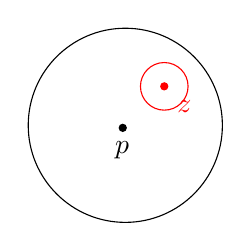
\begin{tikzpicture}[x=0.75pt,y=0.75pt,yscale=-1,xscale=1]
		%uncomment if require: \path (0,117); %set diagram left start at 0, and has height of 117

		%Shape: Circle [id:dp06686904773347901] 
		\draw   (206.46,56.77) .. controls (206.46,30.94) and (227.4,10) .. (253.23,10) .. controls (279.06,10) and (300,30.94) .. (300,56.77) .. controls (300,82.6) and (279.06,103.54) .. (253.23,103.54) .. controls (227.4,103.54) and (206.46,82.6) .. (206.46,56.77) -- cycle ;
		%Shape: Circle [id:dp1943751883500897] 
		\draw  [draw opacity=0][fill={rgb, 255:red, 0; green, 0; blue, 0 }  ,fill opacity=1 ][line width=3]  (250,58) .. controls (250,56.9) and (250.9,56) .. (252,56) .. controls (253.1,56) and (254,56.9) .. (254,58) .. controls (254,59.1) and (253.1,60) .. (252,60) .. controls (250.9,60) and (250,59.1) .. (250,58) -- cycle ;
		%Shape: Circle [id:dp09002262431454922] 
		\draw  [draw opacity=0][fill={rgb, 255:red, 255; green, 0; blue, 0 }  ,fill opacity=1 ][line width=3]  (270,38) .. controls (270,36.9) and (270.9,36) .. (272,36) .. controls (273.1,36) and (274,36.9) .. (274,38) .. controls (274,39.1) and (273.1,40) .. (272,40) .. controls (270.9,40) and (270,39.1) .. (270,38) -- cycle ;
		%Shape: Circle [id:dp04152500828404748] 
		\draw  [color={rgb, 255:red, 255; green, 0; blue, 0 }  ,draw opacity=1 ] (260.53,38) .. controls (260.53,31.67) and (265.67,26.53) .. (272,26.53) .. controls (278.33,26.53) and (283.47,31.67) .. (283.47,38) .. controls (283.47,44.33) and (278.33,49.47) .. (272,49.47) .. controls (265.67,49.47) and (260.53,44.33) .. (260.53,38) -- cycle ;

		% Text Node
		\draw (247,63.4) node [anchor=north west][inner sep=0.75pt]    {$p$};
		% Text Node
		\draw (277,43.4) node [anchor=north west][inner sep=0.75pt]    {$\textcolor[rgb]{1,0,0}{z}$};


		\end{tikzpicture}
	\end{figure}
	\FloatBarrier
	
	Dalla proprietà della media so che 
	\begin{equation*}
		m=u(p) =\frac{1}{| B(p)| }\int _{B(p)} u(y) dy
	\end{equation*}
	\begin{equation*}
		m=\frac{1}{| B(p)| }\left\{\int _{B(p) \backslash B_{r}(z)}\underbrace{u(y)}_{\geqslant m} dy+\int _{B_{r}(z)} u(y) dy\right\}
	\end{equation*}
	Sul secondo termine posso sfruttare ancora la proprietà della media
	\begin{equation*}
		\int _{B_{r}(z)} u(y) dy=u(z)| B_{r(z)}|  >m| B_{r}(z)| 
	\end{equation*}
	Ma allora ottengo una contraddizione
	\begin{equation*}
		m >\frac{1}{| B(p)| }\{m| B(p) \backslash B_{r}(z)| +m| B_{r}(z)| \} =m
	\end{equation*}
	Deduco che $\displaystyle u=m$ in tutto $\displaystyle B(p)$ e quindi anche in $\displaystyle x_{1}$ (poiché $\displaystyle x_{j} \in B(x_{j-1})$) allora posso ripetere il ragionamento che ho fatto trovando $\displaystyle u=m$ in $\displaystyle B(x_{1})$ ed iterando fino all'ultima sfera trovo $\displaystyle u(q) =m$.
\end{dimostrazione}
\subsection{Conseguenze del principio di massimo}

Dal principio di massimo segue come corollario:
\begin{theorem}
	Sia $\displaystyle \Omega $ dominio limitato e $\displaystyle g\in C( \partial \Omega)$. Il problema 
	\begin{equation*}
		\begin{cases}
			\Delta u=0 & \text{in} \ \Omega                   \\
			u=g        & \text{su}\mathrm{\ \partial \Omega } 
		\end{cases}
	\end{equation*}
	ha al massimo una soluzione $\displaystyle u\in C^{2}(\Omega) \cap C(\overline{\Omega \ })$. Inoltre, siano $\displaystyle g_{1},g_{2} \in C( \partial \Omega)$, e $\displaystyle u_{1},u_{2}$ le corrispondenti soluzioni. Allora
	\begin{enumerate}
		\item \textbf{Confronto: }se $\displaystyle g_{1} \geqslant g_{2}$ su $\displaystyle \partial \Omega \ \Rightarrow \ u_{1} \geqslant u_{2}$ su $\displaystyle \Omega $
		\item \textbf{Stabilità }(in norma $\displaystyle L^{\infty }(\Omega)) :$ 
		      \begin{equation}
		      	| u_{1}(x) -u_{2}(x)| \leqslant \max_{\partial \Omega }| g_{1} -g_{2}| \ \forall x\in \overline{\Omega }
		      	\label{eq:lap-stabilita}
		      \end{equation}
	\end{enumerate}
\end{theorem}
\begin{dimostrazione}
	\begin{enumerate}
		\item Sia $\displaystyle w=u_{1} -u_{2} .$Allora $\displaystyle w=g_{1} -g_{2}$ è armonica ed è $\displaystyle \geqslant 0$ su $\displaystyle \partial \Omega $. Poiché $\displaystyle g_{1} -g_{2}$ differiscono in almeno un punto di $\displaystyle \partial \Omega $, $\displaystyle w$ non è costante e per il principio di massimo
		      \begin{equation*}
		      	w(x)  >\min_{\partial \Omega } w(x) =\min_{\partial \Omega } \ (g_{1} -g_{2}) \geqslant 0\ \forall x\in \Omega 
		      \end{equation*}
		      Quindi 
		      \begin{equation*}
		      	w(x) \geqslant 0\ \forall x\in \Omega \ \Rightarrow \ u_{1} \geqslant u_{2} \ \mathrm{su} \ \Omega 
		      \end{equation*}
		\item Sempre dal principio di massimo
		      \begin{gather*}
		      	u_{1}(x) -u_{2}(x) \leqslant \max_{\partial \Omega } \ (g_{1} -g_{2}) \leqslant \max_{\partial \Omega } \ | g_{1} -g_{2}| \\
		      	u_{2}(x) -u_{1}(x) \leqslant \max_{\partial \Omega } \ (g_{2} -g_{1}) \leqslant \max_{\partial \Omega } \ | g_{1} -g_{2}| \\
		      	\Rightarrow \ | u_{1}(x) -u_{2}(x)| \leqslant \max_{\partial \Omega }| g_{1} -g_{2}| 
		      \end{gather*}
		      Ora se $\displaystyle g_{1} =g_{2}$ la \eqref{eq:lap-stabilita} diventa 
		      \begin{equation*}
		      	| u_{1}(x) -u_{2}(x)| =0\ \Rightarrow \ u_{1} =u_{2}
		      \end{equation*}
		      da cui l'unicità.
	\end{enumerate}
\end{dimostrazione}
\textit{Lezione 10 (18/03/2021)}

Se abbiamo $\Delta u=0$ in $\Omega $ ha la proprietà di media in $\Omega $ $\Rightarrow $ principio di massimo $\Rightarrow $ unicità per il problema di Dirichlet.
\section{Laplaciano in coordinate cilindriche}

Consideriamo $p_{1} =p_{2} =0$ per comodità.
\begin{equation*}
\begin{pmatrix}
x\\
y
\end{pmatrix} =\begin{pmatrix}
r\cos \vartheta \\
r\sin \vartheta 
\end{pmatrix} \ \ \Leftrightarrow \ \ r=\sqrt{x^{2} +y^{2}},\ \ \tan \vartheta =\frac{y}{x}
\end{equation*}
Derivando $r,\vartheta $
\begin{align*}
r_{x} & =\cos \vartheta  & r_{y} & =\sin \vartheta \\
\vartheta _{x} & =-\frac{\sin \vartheta }{r} & \vartheta _{y} & =\frac{\cos \vartheta }{r}\\
 &  &  & \\
r_{xx} & =\frac{\sin^{2} \vartheta }{r} & r_{yy} & =\frac{\cos^{2} \vartheta }{r}\\
\vartheta _{xx} & =\frac{2\cos \vartheta \sin \vartheta }{r^{2}} & \vartheta _{yy} & =-\frac{2\cos \vartheta \sin \vartheta }{r^{2}}
\end{align*}
Possiamo derivare $u(r,\vartheta)$ una prima volta
\begin{equation*}
\begin{aligned}
u_{x} & =u_{r} r_{x} +u_{\vartheta } \vartheta _{x}\\
 & =\cos \vartheta u_{r} -\frac{\sin \vartheta }{r} u_{\vartheta }\\
u_{y} & =u_{r} r_{y} +u_{\vartheta } \vartheta _{y}\\
 & =\sin \vartheta u_{r} +\frac{\cos \vartheta }{r} u_{\vartheta }
\end{aligned}
\end{equation*}
e una seconda volta
\begin{equation*}
\begin{aligned}
u_{xx} & =u_{rx} r_{x} +u_{r} r_{xx} +u_{\vartheta x} \vartheta _{x} +u_{\vartheta } \vartheta _{xx}\\
 & =u_{rr} r^{2}_{x} +2u_{r\vartheta } r_{x} \vartheta _{x} +u_{r} r_{xx} +u_{\vartheta \vartheta } \vartheta ^{2}_{x} +u_{\vartheta } \vartheta _{xx}\\
 & =\cos^{2} \vartheta u_{rr} -\frac{2\cos \vartheta \sin \vartheta }{r} u_{r\vartheta } +\frac{\sin^{2} \vartheta }{r} u_{r} +\frac{\sin^{2} \vartheta }{r^{2}} u_{\vartheta \vartheta } +\frac{2\cos \vartheta \sin \vartheta }{r^{2}} u_{\vartheta }\\
u_{yy} & =u_{ry} r_{y} +u_{r} r_{yy} +u_{\vartheta y} \vartheta _{y} +u_{\vartheta } \vartheta _{yy}\\
 & =u_{rr} r^{2}_{y} +2u_{r\vartheta } r_{y} \vartheta _{y} +u_{r} r_{yy} +u_{\vartheta \vartheta } \vartheta ^{2}_{y} +u_{\vartheta } \vartheta _{yy}\\
 & =\sin^{2} \vartheta u_{rr} +\frac{2\cos \vartheta \sin \vartheta }{r} u_{r\vartheta } +\frac{\cos^{2} \vartheta }{r} u_{r} +\frac{\cos^{2} \vartheta }{r^{2}} u_{\vartheta \vartheta } -\frac{2\cos \vartheta \sin \vartheta }{r^{2}} u_{\vartheta } .
\end{aligned}
\end{equation*}
mettendo insieme otteniamo
\begin{equation*}
\nabla ^{2} u=u_{rr} +\frac{1}{r} u_{r} +\frac{1}{r^{2}} u_{\vartheta \vartheta }
\end{equation*}
\section{Formula di Poisson per il cerchio}
\begin{theorem}
L'\textbf{unica} soluzione $u\in C^{2}(B_{R}(p)) \cap C\left(\overline{B_{R}(p)}\right)$ del problema di Dirichlet
\begin{equation*}
\begin{cases}
\Delta u=0, & \text{in} \ B_{R}(p)\\
u=g, & \text{su} \ \partial B_{R}(p)
\end{cases}
\end{equation*}
dove $g$ è continua sul bordo $g\in C( \partial B_{R}(p))$, è data dalla \textbf{Formula di Poisson}
\begin{equation*}
u(x) =\frac{R^{2} -| x-p| ^{2}}{2\pi R}\int _{\partial B_{R}(p)}\frac{g(\sigma)}{| x-\sigma | ^{2}} d\sigma 
\end{equation*}
\end{theorem}
\begin{dimostrazione}
L'unicità segue dal principio di massimo. Passiamo in coordinate polari
\begin{equation*}
x=(x_{1},x_{2}) \ \ \Rightarrow \ \ \begin{cases}
x_{1} =p_{1} +r\cos \vartheta \\
x_{2} =p_{2} +r\sin \vartheta 
\end{cases}
\end{equation*}
Le funzioni del problema diventano
\begin{gather*}
U(r,\vartheta) =u( p_{1} +r\cos \vartheta,p_{2} +r\sin \vartheta)\\
G(\vartheta) =g( p_{1} +R\cos \vartheta,p_{2} +R\sin \vartheta)
\end{gather*}
L'equazione $\Delta u=0$ in $B_{R}(p)$ diventa\footnote{si veda la sezione precedente.}
\begin{equation*}
U_{rr} +\frac{1}{r} U_{r} +\frac{1}{r^{2}} U_{\vartheta \vartheta } =0,\ \ \ \ \text{in} \ 0< r< R,\ \ 0\leqslant \vartheta \leqslant 2\pi 
\end{equation*}
La condizione di Dirichlet diventa
\begin{equation*}
U(R,\vartheta) =G(\vartheta),\ \ \ \ 0\leqslant \vartheta \leqslant 2\pi 
\end{equation*}
Deve inoltre essere:
\begin{gather*}
U\ \text{continua in} \ [ 0,R] \times [ 0,2\pi ]\\
G\ \text{continua in} \ [ 0,2\pi ]
\end{gather*}
e periodiche di periodo $2\pi $.

Usiamo il \textbf{metodo di separazione delle variabili}, cerchiamo soluzioni della forma
\begin{equation}
U(r,\vartheta) =v(r) w(\vartheta)
\label{eq:poisson-cerchio-6-sep-var}
\end{equation}
con $v,w$ continue in $[ 0,R]$ e $[ 0,2\pi ]$ rispettivamente e $w$ funzione $2\pi $-periodica. Sostituendo
\begin{equation*}
v''(r) w(\vartheta) +\frac{1}{r} v'(r) w(\vartheta) +\frac{1}{r^{2}} v(r) w''(\vartheta) =0
\end{equation*}
dividiamo per $v(r) w(\vartheta)$ e separiamo
\begin{equation*}
-\frac{r^{2} v''(r) +rv'(r)}{v(r)} =\frac{w''(\vartheta)}{w(\vartheta)} =\lambda \ \text{costante}
\end{equation*}
La trattazione si spezza in due sottoproblemi
\begin{align*}
(1) & \ \ r^{2} v''(r) +rv'(r) +\lambda v(r) =0\\
(2) & \ \ \begin{cases}
w''(\vartheta) -\lambda w(\vartheta) =0\ \text{in} \ (0,2\pi)\\
w(0) =w(2\pi)
\end{cases}
\end{align*}

\begin{enumerate}
\item [(2)] se $\lambda \geqslant 0$ non ci sono soluzioni non banali
\begin{enumerate}
\item $\lambda  >0$, allora\begin{equation*}
w(\vartheta) =ae^{-\sqrt{\lambda } \vartheta } +be^{\sqrt{\lambda } \vartheta }
\end{equation*}nessuna scelta di $a,b$ mi dà soluzioni periodiche.
\item $\lambda =0$, allora\begin{equation*}
w(\vartheta) =a\vartheta +b\ \ \Rightarrow \ \ a=b=0
\end{equation*}la soluzione è banale.
\end{enumerate}

consideriamo quindi solo il caso $\lambda =-\mu ^{2}$, $\mu  >0$, l'integrale generale sarà\begin{equation*}
w(\vartheta) =a\cos \mu \vartheta +b\sin \mu \vartheta,\ \ \ \ a,b\in \mathbb{R}
\end{equation*}la periodicità implica che $\mu $ deve essere intero $\mu =m=0,1,2\dotsc $
\item [(1)] Qui vi è un'equazione di Eulero
\begin{equation}
r^{2} v''(r) +rv'(r) -m^{2} v(r) =0
\label{eq:poisson-cerchio-5-eq-eulero}
\end{equation}
Poniamo $s=\log r$, ossia $r=e^{s}$, e poniamo $z(s) =v\left(e^{s}\right)$, allora\footnote{ricordando che l'argomento è $e^{s} =r$.}\begin{equation*}
\begin{array}{ l }
\Rightarrow \ \ z'(s) =v'\left(e^{s}\right) \cdotp e^{s} =v'(r) r\\
\Rightarrow \ \ z''(s) =v''\left(e^{s}\right) e^{2s} +v'\left(e^{s}\right) e^{s} =v''(r) r^{2} +v'(r) r
\end{array}
\end{equation*}

pertanto nella \eqref{eq:poisson-cerchio-5-eq-eulero} ci siamo ricondotti a un problema agli autovalori\begin{equation*}
z''(s) -m^{2} z(s) =0\ \ \Rightarrow \ \ z(s) =c_{1} e^{-ms} +c_{2} e^{ms}
\end{equation*}

tornando alla funzione $v$ e ricordando che $r=e^{s}$\begin{equation*}
v(r) =\cancel{c_{1} r^{-m}} +c_{2} r^{m} \ \ \ \ 0< r< R
\end{equation*}elidiamo il primo termine poichè $v$ deve essere continua nel cerchio, se quel termine fosse presente, sarebbe illimitata nell'origine.
\end{enumerate}

Abbiamo così le infinite soluzioni armoniche sostituendo le due soluzioni in \eqref{eq:poisson-cerchio-6-sep-var}
\begin{equation*}
U_{m}(r,\vartheta) =r^{m}\{a_{m}\cos m\vartheta +b_{m}\sin m\vartheta \},\ \ \ \ m=0,1,2\dotsc 
\end{equation*}
sovrapponendo le quali abbiamo la candidata soluzione
\begin{equation}
U(r,\vartheta) =a_{0} +\sum\limits ^{\infty }_{m=1} r^{m}\{a_{m}\cos m\vartheta +b_{m}\sin m\vartheta \}
\label{eq:poisson-cerchio-3-candidata}
\end{equation}
con la condizione
\begin{equation}
\lim _{(r,\vartheta)\rightarrow (R,\xi)} U(r,\vartheta) =G(\xi),\ \ \ \ \forall \xi \in [ 0,2\pi ]
\label{eq:poisson-cerchio-2-condizione}
\end{equation}
\textbf{Limitiamoci ora a studiare il caso con }$G\in C^{1}([ 0,2\pi ])$

Si può sviluppare $G$ in serie di Fourier
\begin{equation}
G(\xi) =\frac{\alpha _{0}}{2} +\sum\limits ^{\infty }_{m=1}\{\alpha _{m}\cos m\vartheta +\beta _{m}\sin m\vartheta \} \tag{F}
\label{eq:poisson-cerchio-4-bordo-fourier}
\end{equation}
dove
\begin{equation*}
\alpha _{m} =\frac{1}{\pi }\int ^{2\pi }_{0} G(\varphi)\cos m\varphi \ d\varphi \ \ \ \ \beta _{m} =\frac{1}{\pi }\int ^{2\pi }_{0} G(\varphi)\sin m\varphi \ d\varphi 
\end{equation*}
ed essendo $G\in C^{1}([ 0,2\pi ])$ abbiamo
\begin{equation*}
\sum\limits ^{\infty }_{m=1}| \alpha _{m}| \ \ \ \ \sum\limits ^{\infty }_{m=1}| \beta _{m}| \ \ \ \ \text{convergenti}
\end{equation*}
allora la serie di Fourier \eqref{eq:poisson-cerchio-4-bordo-fourier} è unformemente convergente in $[ 0,2\pi ]$.

La \eqref{eq:poisson-cerchio-2-condizione} è soddisfatta purché scegliamo
\begin{equation*}
a_{0} =\frac{\alpha _{0}}{2} \ \ \ \ a_{m} =R^{-m} \alpha _{m} \ \ \ \ b_{m} =R^{-m} \beta _{m}
\end{equation*}
Sostituendo nella \eqref{eq:poisson-cerchio-3-candidata}
\begin{equation*}
U(r,\vartheta) =\frac{\alpha _{0}}{2} +\frac{1}{\pi }\sum\limits ^{\infty }_{m=1}\left(\frac{r}{R}\right)^{m}\int ^{2\pi }_{0} G(\varphi)\underbrace{\{\cos m\varphi \cos m\vartheta +\sin m\varphi \sin m\vartheta \}}_{\cos m( \varphi -\vartheta)} d\varphi 
\end{equation*}
Per $r< R$, grazie alla convergenza uniforme della serie possiamo scambiare serie e integrale
\begin{equation*}
U(r,\vartheta) =\sum \int =\int \sum 
\end{equation*}
Notiamo anche che
\begin{equation*}
\frac{\alpha _{0}}{2} =\frac{1}{2\pi }\int ^{2\pi }_{0} G(\varphi) d\varphi 
\end{equation*}
in questo modo possiamo sviluppare ulteriormente il termine accorpando tutto dentro un unico integrale e raccogliendo $\frac{1}{\pi }$
\begin{align}
U(r,\vartheta) & =\frac{1}{2\pi }\int ^{2\pi }_{0} G(\varphi) d\varphi +\int ^{2\pi }_{0}\frac{1}{\pi }\sum\limits ^{\infty }_{m=1}\left(\frac{r}{R}\right)^{m} G(\varphi)\cos m( \varphi -\vartheta) d\varphi \nonumber\\
 & =\frac{1}{\pi }\int ^{2\pi }_{0} G(\varphi)\left\{\frac{1}{2} +\sum\limits ^{\infty }_{m=1}\left(\frac{r}{R}\right)^{m}\cos m( \varphi -\vartheta)\right\} d\varphi \nonumber\\
 & =\frac{1}{\pi }\int ^{2\pi }_{0} G(\varphi)\left\{\frac{1}{2} -1+1+\sum\limits ^{\infty }_{m=1}\left(\frac{r}{R}\right)^{m}\cos m( \varphi -\vartheta)\right\} d\varphi \nonumber\\
 & =\frac{1}{\pi }\int ^{2\pi }_{0} G(\varphi)\left\{-\frac{1}{2} +\sum\limits ^{\infty }_{m=0}\left(\frac{r}{R}\right)^{m}\cos m( \varphi -\vartheta)\right\} d\varphi \label{eq:poisson-cerchio-1}
\end{align}
Nell'ultimo passaggio abbiamo aggiunto il termine $1$ per far partire la serie da $m=0$. Notiamo che la serie può essere vista come la parte reale di una serie geometrica
\begin{equation*}
\sum\limits ^{\infty }_{m=0}\left(\frac{r}{R}\right)^{m}\cos m( \varphi -\vartheta) =\mathrm{Re}\left[\sum\limits ^{\infty }_{m=0}\left(\frac{r}{R} e^{i( \varphi -\vartheta)}\right)^{m}\right]
\end{equation*}
Che possiamo sviluppare
\begin{align*}
\mathrm{Re}\left[\sum\limits ^{\infty }_{m=0}\left(\frac{r}{R} e^{i( \varphi -\vartheta)}\right)^{m}\right] & =\mathrm{Re}\left[\frac{1}{1-\frac{r}{R} e^{i( \varphi -\vartheta)}}\right]\\
 & =\mathrm{Re}\left[ R\frac{1}{R-r(\cos( \varphi -\vartheta) +i\sin( \varphi -\vartheta))}\right]\\
 & =\mathrm{Re}\left[ R\frac{1}{R-r\cos( \varphi -\vartheta) +ir\sin( \varphi -\vartheta)}\right]\\
 & =\mathrm{Re}\left[ R\frac{R-r\cos( \varphi -\vartheta) -ir\sin( \varphi -\vartheta)}{( R-r\cos( \varphi -\vartheta))^{2} -i^{2} r^{2}\sin^{2}( \varphi -\vartheta)}\right]\\
 & =R\frac{R-r\cos( \varphi -\vartheta)}{R^{2} +r^{2}\cos^{2}( \varphi -\vartheta) -2rR\cos( \varphi -\vartheta) +r^{2}\sin^{2}( \varphi -\vartheta)}\\
 & =R\frac{R-r\cos( \varphi -\vartheta)}{R^{2} +r^{2} -2rR\cos( \varphi -\vartheta)}
\end{align*}
possiamo sostituire nella \eqref{eq:poisson-cerchio-1}
\begin{align*}
U(r,\vartheta) & =\frac{1}{\pi }\int ^{2\pi }_{0} G(\varphi)\left\{-\frac{1}{2} +\frac{R^{2} -rR\cos( \varphi -\vartheta)}{R^{2} +r^{2} -2rR\cos( \varphi -\vartheta)}\right\} d\varphi \\
 & =\frac{1}{\pi }\int ^{2\pi }_{0} G(\varphi)\left\{\frac{-\left( R^{2} +r^{2} -2rR\cos( \varphi -\vartheta)\right) +2R^{2} -2rR\cos( \varphi -\vartheta)}{2\left( R^{2} +r^{2} -2rR\cos( \varphi -\vartheta)\right)}\right\} d\varphi \\
 & =\frac{1}{2\pi }\int ^{2\pi }_{0} G(\varphi)\left\{\frac{R^{2} -r^{2}}{R^{2} +r^{2} -2rR\cos( \varphi -\vartheta)}\right\} d\varphi \\
 & =\frac{R^{2} -r^{2}}{2\pi }\int ^{2\pi }_{0}\frac{G(\varphi)}{R^{2} +r^{2} -2rR\cos( \varphi -\vartheta)} d\varphi 
\end{align*}
Osserviamo che il valore al centro del cerchio
\begin{equation*}
u(0,0) =\frac{1}{2\pi }\int ^{2\pi }_{0} G(\varphi) d\varphi 
\end{equation*}
non è altro che la media dei valori assunti da $G$ sul bordo.

Tornando alle variabili originali\footnote{Denotiamo con $\mathbf{p} =\begin{pmatrix}
p_{1}\\
p_{2}
\end{pmatrix}$ il centro del cerchio, con $\mathbf{\sigma } =\begin{pmatrix}
p_{1} +R\cos \varphi \\
p_{2} +R\sin \varphi 
\end{pmatrix}$ un punto sul bordo, con $\mathbf{x} =\begin{pmatrix}
p_{1} +r\cos \vartheta \\
p_{2} +r\sin \vartheta 
\end{pmatrix}$ un punto del cerchio. Il differenziale si trova come determinante dello Jacobiano $d\mathbf{\sigma } =Rd\varphi $. Questo ci permette anche di riscrivere il denominatore
\begin{align*}
| \mathbf{x} -\mathbf{\sigma }| ^{2} & =( R\cos \varphi -r\cos \vartheta)^{2} +( R\sin \varphi -r\sin \vartheta)^{2}\\
 & =R^{2}\cos^{2} \varphi +r^{2}\cos^{2} \vartheta -2rR\cos \varphi \cos \vartheta +R^{2}\sin^{2} \varphi +r^{2}\sin^{2} \vartheta -2rR\sin \varphi \sin \vartheta \\
 & =R^{2} +r^{2} -2rR(\cos \varphi \cos \vartheta -\sin \varphi \sin \vartheta)\\
 & =R^{2} +r^{2} -2rR\cos( \varphi -\vartheta)
\end{align*}}
\begin{equation}
u(\mathbf{x}) =\frac{R^{2} -| \mathbf{x} -\mathbf{p}| ^{2}}{2\pi R}\int _{\partial B_{R}(\mathbf{p})}\frac{g(\mathbf{\sigma })}{| \mathbf{x} -\mathbf{\sigma }| ^{2}} d\sigma 
\label{eq:poisson-cerchio}
\end{equation}
Se $\mathbf{x} \in B_{R}(\mathbf{p})$, cioè dentro e non sul bordo



\begin{figure}[H]
	\centering

	\tikzset{every picture/.style={line width=0.75pt}} %set default line width to 0.75pt        

	\begin{tikzpicture}[x=0.75pt,y=0.75pt,yscale=-1,xscale=1]
	%uncomment if require: \path (0,138); %set diagram left start at 0, and has height of 138

	%Curve Lines [id:da3646608908276512] 
	\draw    (253,4.63) .. controls (292,24.63) and (318,78.63) .. (313,133.63) ;
	%Shape: Circle [id:dp25903533863346984] 
	\draw  [dash pattern={on 0.84pt off 2.51pt}] (222,72) .. controls (222,54.88) and (235.88,41) .. (253,41) .. controls (270.12,41) and (284,54.88) .. (284,72) .. controls (284,89.12) and (270.12,103) .. (253,103) .. controls (235.88,103) and (222,89.12) .. (222,72) -- cycle ;
	%Shape: Circle [id:dp6902212722781198] 
	\draw  [draw opacity=0][fill={rgb, 255:red, 0; green, 0; blue, 0 } ,fill opacity=1 ] (251,72) .. controls (251,70.9) and (251.9,70) .. (253,70) .. controls (254.1,70) and (255,70.9) .. (255,72) .. controls (255,73.1) and (254.1,74) .. (253,74) .. controls (251.9,74) and (251,73.1) .. (251,72) -- cycle ;

	% Text Node
	\draw (317,66.4) node [anchor=north west][inner sep=0.75pt]    {$\partial B_{R}(\mathbf{p})$};
	% Text Node
	\draw (255,73.4) node [anchor=north west][inner sep=0.75pt]    {$\mathbf{x}$};


	\end{tikzpicture}

\end{figure}
\FloatBarrier

possiamo passare al limite sotto il segno di integrale perché il denominatore non si annulla mai, e in particolare risulta $u\in C^{\infty }(B_{R}(p))$

\textbf{Caso con }$G\in C([ 0,2\pi ])$, solamente continua. La \eqref{eq:poisson-cerchio} definisce $u\in C^{\infty }(B_{R}(p))$ e armonica in $B_{R}(p)$. L'unica cosa un po' delicata sono le condizioni al bordo, che comunque si possono verificare.

\end{dimostrazione}

\textit{Lezione 11 (22/03/2021)}

Possiamo generalizzare la (16) per un numero generico $\displaystyle n$ di dimensioni
\begin{equation*}
	u(\mathbf{x}) =\frac{R^{2} -| \mathbf{x} -\mathbf{p}| ^{2}}{w_{n} R}\int _{\partial B_{R}(\mathbf{p})}\frac{g(\mathbf{\sigma })}{| \mathbf{x} -\mathbf{\sigma }| ^{n}} d\mathbf{\sigma }
\end{equation*}
con $\displaystyle u\in C^{\infty }( B_{R}(\mathbf{p})) \cap C\left(\overline{B_{R}}(\mathbf{p})\right)$.
\section{Soluzione fondamentale per l'operatore di Laplace}

Come abbiamo trovato e costruito una soluzione fondamentale per l'operatore del calore, cerchiamo una soluzione con proprietà simili per l'operatore di Laplace: questa soluzione fondamentale, armonica in tutto $\displaystyle \mathbb{R}^{n}$ tranne che in un punto, ci servirà per costruire una formula di rappresentazione per la soluzione del problema di Dirichlet che coinvolge dei potenziali.

Sia $\displaystyle u=u(x)$ armonica in $\displaystyle \mathbb{R}^{n}$ e sia $\displaystyle M$ una matrice di rotazione, cioè tale che
\begin{equation*}
	M^{T} =M^{-1} \ \ \land \ \ \mathrm{det} M=1
\end{equation*}
Iniziamo osservando che, definita $\displaystyle D^{2} u$ l'Hessiana di $\displaystyle u$, possiamo scrivere
\begin{equation*}
	\Delta u=\mathrm{Tr} D^{2} u
\end{equation*}
Definiamo $\displaystyle v(x) =u(Mx)$, allora
\begin{equation*}
	D^{2} v(x) =M^{T} D^{2} u(Mx) M
\end{equation*}
inoltre
\begin{align*}
	\Delta v(x) & =\mathrm{Tr}\left[ M^{T} D^{2} u(Mx) M\right] &                                        \\
	             & =\mathrm{Tr} D^{2} u(Mx)                      & M\ \text{ortogonale non varia traccia} \\
	             & =\Delta u(Mx) =0                              &                                        
\end{align*}
$\displaystyle v$ è ancora armonica: il Laplaciano commuta con le rotazioni e dunque $\displaystyle \Delta $ è invariante per rotazioni. Si dimostra facilmente che $\displaystyle \Delta $ è anche invariante per traslazione: se $\displaystyle u(x)$ è armonica, $\displaystyle v(x) =u(x-y)$, per ogni $\displaystyle y$ fissato, è armonica.

Per l'operatore del calore la soluzione fondamentale (in $\displaystyle n=3$) era
\begin{equation*}
	\Gamma _{D}(x,t) =\frac{1}{(4\pi Dt)^{3/2}}\exp\left\{-\frac{\textcolor[rgb]{0.82,0.01,0.11}{| }\textcolor[rgb]{0.82,0.01,0.11}{x}\textcolor[rgb]{0.82,0.01,0.11}{| }\textcolor[rgb]{0.82,0.01,0.11}{^{2}}}{4D\textcolor[rgb]{0.82,0.01,0.11}{t}}\right\}
\end{equation*}
Il blocco $\displaystyle \textcolor[rgb]{1,0,0}{\frac{| x| ^{2}}{t}}$ è invariante per dilatazioni paraboliche della forma
\begin{align*}
	x & \longmapsto ax      \\
	t & \longmapsto a^{2} t 
\end{align*}
Dove il tempo \textit{conta} come il quadrato dello spazio: questo non è altro che il riflesso dell'operatore del calore stesso, dove una derivata temporale \textit{compensava} una derivata seconda spaziale	
\begin{equation*}
	u_{t} -Du_{xx} =0
\end{equation*}
Ci aspettiamo per analogia che, essendo l'operatore di Laplace invariante per rotazioni, anche la soluzione fondamentale per l'operatore Laplaciano sia invariante per rotazioni. Cerchiamo quindi una soluzione della forma
\begin{equation*}
	u=u(| x|)
\end{equation*}
Poniamo $\displaystyle r=| x| $ e cerchiamo $\displaystyle u=u(r)$ tale che
\begin{equation*}
	\Delta u=0\ \text{in} \ \mathbb{R}^{n} \setminus \{0\},\ n=2,3
\end{equation*}
In $\displaystyle 0$ non può essere armonica perché non è derivabile. Dato che la soluzione è radiale conviene passare alle coordinate polari
\begin{itemize}
	\item $\displaystyle n=2$\begin{equation*}
	      \Delta _{\text{polare}} u(r) =u_{rr} +\frac{1}{r} u_{r} +\cancel{\frac{1}{r^{2}} u_{\vartheta \vartheta }} =0
	\end{equation*}
	
	Risolvendo separando le variabili\begin{align*}
	\frac{u_{rr}}{u_{r}} & =-\frac{1}{r}\\
	\log| u_{r}|  & =-\log r+c_{1}
	\end{align*}
	
	Definendo $\displaystyle k=e^{c_{1}}  >0$\begin{equation*}
	| u_{r}| =k\frac{1}{r}
	\end{equation*}
	
	Liberandoci infine del modulo ($\displaystyle k\in \mathbb{R}$)\begin{equation*}
	u_{r} =k\frac{1}{r}
	\end{equation*}
	
	Otteniamo la soluzione\begin{equation*}
	\boxed{u(r) =k\log r+k_{1}} \ \ (r\neq 0)
	\end{equation*}
	\item $\displaystyle n=3$\begin{align*}
	      \Delta _{\text{sferico}} u(r) =u_{rr} +\frac{2}{r} u_{r} & =0\\
	      (ru)_{rr} & =0\\
	      ru & =Ar+B
	\end{align*}
	
	Che dà come soluzione\begin{equation*}
	\boxed{u(r) =A+\frac{B}{r}}
	\end{equation*}
\end{itemize}

Per ottenere la soluzione fondamentale devo scegliere le costanti in modo tale che\footnote{Il procedimento per la scelta delle costanti sarà svolto nella parte di analisi funzionale.} 
\begin{equation*}
	-\Delta u=\delta _{n} \ \text{in} \ \mathbb{R}^{n}
\end{equation*}
Da cui ricaviamo la \textbf{soluzione fondamentale}
\begin{equation*}
	\Phi (x) =\begin{cases}
	-\frac{1}{2\pi }\log| x|  & n=2\\
	\frac{1}{4\pi | x| } & n=3
	\end{cases}
\end{equation*}
$\displaystyle \Phi $ è definita per $\displaystyle x\neq 0$ e ha significato fisico. Se $\displaystyle n=3$, $\displaystyle 4\pi \Phi $ rappresenta il potenziale elettrostatico generato da una carica posta nell'origine che si annulla all'infinito. Se $\displaystyle n=2$, $\displaystyle 2\pi \Phi $ rappresenta il potenziale generato da una carica di densità totale $\displaystyle 1$, distribuita lungo l'asse $\displaystyle x_{3}$.

Se la carica è posta in un punto $\displaystyle y$ fissato possiamo sfruttare l'invarianza per traslazione 
\begin{equation*}
	\Delta _{x} \Phi (x-y) =-\delta _{y}
\end{equation*}
E per simmetria, con $\displaystyle x$ fissato
\begin{equation*}
	\Delta _{y} \Phi (x-y) =-\delta _{x}
\end{equation*}
Generalizzando per dimensione $\displaystyle n >3$ la soluzione fondamentale è
\begin{equation*}
	\Phi (x) =\frac{1}{(n-2) w_{n}}\frac{1}{| x| ^{n-2}}
\end{equation*}
\section{Il potenziale Newtoniano}

Torniamo in dimensione $\displaystyle n=3$. Supponiamo che $\displaystyle \frac{1}{4\pi } f(y)$ rappresenti la densità di una carica localizzata all'interno di un compatto di $\displaystyle \mathbb{R}^{3}$. Il potenziale in $\displaystyle x$ generato dalla carica presente in un piccolo volumetto $\displaystyle dy$, centrata in $\displaystyle y$, è dato da
\begin{equation*}
	\Phi (x-y) f(y) dy
\end{equation*}
Il potenziale totale si ottiene integrando
\begin{equation*}
	\mathcal{N}_{f}(x) =\int _{\mathbb{R}^{3}} \Phi (x-y) f(y) dy=\frac{1}{4\pi }\int _{\mathbb{R}^{3}}\frac{f(y)}{| x-y| } dy=(\Phi \ast f)(x)
\end{equation*}
Questo potenziale è detto \textbf{potenziale Newtoniano} di $\displaystyle f$. Formalmente, nel senso delle distribuzioni e sotto opportune ipotesi per $\displaystyle f$\footnote{Per $\displaystyle x$ fissato $\displaystyle \frac{1}{| x-y| } \in L^{1}(B(0))$, quindi dovrò controllare solo il comportamento di $\displaystyle f(y)$.}:
\begin{equation*}
	-\Delta \mathcal{N}_{f}(x) =( -\Delta \Phi \ast f)(x) =( \delta _{3} \ast f)(x) =\int _{\mathbb{R}^{3}} \delta _{3}(x-y) f(y) dy=f(x)
\end{equation*}
\begin{theorem}
	Sia $\displaystyle f\in C^{2}\left(\mathbb{R}^{3}\right)$ a supporto compatto. Allora $\displaystyle \mathcal{N}_{f} \in C^{2}\left(\mathbb{R}^{3}\right)$ ed è l'unica soluzione dell'equazione di Poisson
	\begin{equation*}
		-\Delta u=f\ \text{in} \ \mathbb{R}^{3}
	\end{equation*}
	che si annulla all'infinito.
\end{theorem}
\begin{nb}
	Per $\displaystyle n=2$ il potenziale Newtoniano si chiama potenziale logaritmico
	\begin{equation*}
		\mathcal{L}_{f}(x) =-\frac{1}{2\pi }\int _{\mathbb{R}^{2}}\log| x-y| f(y) dy
	\end{equation*}
	e vale un risultato simile: se $\displaystyle f\in C^{2}$, $\displaystyle \mathcal{L}_{f} \in C^{2}$ ed è l'unica soluzione di 
	\begin{equation*}
		-\Delta u=f\ \text{in} \ \mathbb{R}^{2}
	\end{equation*}
	con andamento asintotico
	\begin{equation*}
		u(x) =-\frac{M}{2\pi }\log| x| +o\left(\frac{1}{| x| }\right),\ | x| \rightarrow +\infty 
	\end{equation*}
	Dove $\displaystyle M$ è la carica totale
	\begin{equation*}
		M=\int _{\mathbb{R}^{2}} f(y) dy
	\end{equation*}
\end{nb}
\section{La funzione di Green}
\begin{theorem}
	Sia $\displaystyle \Omega \subset \mathbb{R}^{3}$ un dominio limitato e regolare, sia $\displaystyle u\in C^{2}(\overline{\Omega }$). Allora:
	\begin{equation*}
		u(x) =\underbrace{-\int _{\Omega } \Phi (x-y) \Delta u(y) dy}_{ \begin{array}{l}
			\text{potenziale Newtoniano di}\\
			f=\Delta u
			\end{array}} +\underbrace{\int _{\partial \Omega } \Phi (x-y) \partial _{\nu } u(\sigma) d\sigma }_{ \begin{array}{l}
			\text{potenziale di strato semplice}\\
			\text{con densità} \ \partial _{\nu } u
			\end{array}}\underbrace{-\int _{\partial \Omega } \partial _{\nu } \Phi (x-\sigma) u(\sigma) d\sigma }_{ \begin{array}{l}
			\text{potenziale di doppio strato}\\
			\text{con momento} \ \mu 
			\end{array}}
	\end{equation*}
\end{theorem}
In pratica, ogni funzione regolare $\displaystyle u$ può essere scritta come somma di un potenziale di volume (Newtoniano) con densità $\displaystyle -\Delta u$, di un potenziale di strato semplice causato da una densità di cariche $\displaystyle \partial _{\nu } u$ sulla $\displaystyle \partial \Omega $ e da un potenziale di doppio strato generato da dei dipoli elettrici con momento $\displaystyle \mu $.

Vediamo la dimostrazione del teorema.
\begin{dimostrazione}
	Ricordiamo innanzitutto l'identità di Green con $\displaystyle u,v\in C^{2}(\overline{\Omega })$
	\begin{equation*}
		\int _{\Omega }( v\Delta u-u\Delta v) dx=\int _{\partial \Omega }( v\partial _{\nu } u-u\partial _{\nu } v) d\sigma 
	\end{equation*}
	Applichiamo l'identità di Green utilizzando come funzione $\displaystyle u$ la stessa dell'enunciato del teorema. Per la funzione $\displaystyle v$ dobbiamo trovare un'alternativa, infatti, con $\displaystyle x$ fissato
	\begin{equation*}
		v(y) =\Phi (x-y) =\frac{1}{4\pi }\frac{1}{| x-y| } \notin C^{2}(\Omega)
	\end{equation*}
	Con $\displaystyle \Omega $ dominio limitato, definisco 
	\begin{equation*}
		\Omega _{\varepsilon } =\Omega \setminus \overline{B}_{\varepsilon }(x)
	\end{equation*}
	
	\begin{figure}[H]
		\centering
		\tikzset{every picture/.style={line width=0.75pt}} %set default line width to 0.75pt        

		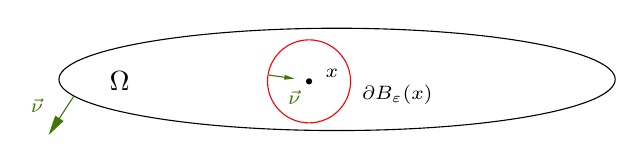
\begin{tikzpicture}[x=0.75pt,y=0.75pt,yscale=-1,xscale=1]
		%uncomment if require: \path (0,86); %set diagram left start at 0, and has height of 86

		%Shape: Ellipse [id:dp8534708959725636] 
		\draw   (100,39.65) .. controls (100,26.04) and (159.99,15) .. (234,15) .. controls (308.01,15) and (368,26.04) .. (368,39.65) .. controls (368,53.27) and (308.01,64.3) .. (234,64.3) .. controls (159.99,64.3) and (100,53.27) .. (100,39.65) -- cycle ;
		%Shape: Ellipse [id:dp5474821128070129] 
		\draw  [draw opacity=0][fill={rgb, 255:red, 0; green, 0; blue, 0 }  ,fill opacity=1 ][line width=3]  (222,40.6) .. controls (222,39.77) and (221.33,39.1) .. (220.5,39.1) .. controls (219.67,39.1) and (219,39.77) .. (219,40.6) .. controls (219,41.43) and (219.67,42.1) .. (220.5,42.1) .. controls (221.33,42.1) and (222,41.43) .. (222,40.6) -- cycle ;
		%Shape: Ellipse [id:dp9123452672283427] 
		\draw  [color={rgb, 255:red, 251; green, 0; blue, 0 }  ,draw opacity=1 ] (200.5,40.6) .. controls (200.5,29.55) and (209.45,20.6) .. (220.5,20.6) .. controls (231.55,20.6) and (240.5,29.55) .. (240.5,40.6) .. controls (240.5,51.65) and (231.55,60.6) .. (220.5,60.6) .. controls (209.45,60.6) and (200.5,51.65) .. (200.5,40.6) -- cycle ;
		%Straight Lines [id:da4961016004934615] 
		\draw [color={rgb, 255:red, 65; green, 117; blue, 5 }  ,draw opacity=1 ]   (107.2,47.65) -- (96.09,64.79) ;
		\draw [shift={(95,66.47)}, rotate = 302.96] [fill={rgb, 255:red, 65; green, 117; blue, 5 }  ,fill opacity=1 ][line width=0.08]  [draw opacity=0] (9.6,-2.4) -- (0,0) -- (9.6,2.4) -- cycle    ;
		%Straight Lines [id:da17326606651197296] 
		\draw [color={rgb, 255:red, 65; green, 117; blue, 5 }  ,draw opacity=1 ]   (201.2,37.58) -- (211.42,38.99) ;
		\draw [shift={(213.4,39.27)}, rotate = 187.85] [fill={rgb, 255:red, 65; green, 117; blue, 5 }  ,fill opacity=1 ][line width=0.08]  [draw opacity=0] (4.8,-1.2) -- (0,0) -- (4.8,1.2) -- cycle    ;

		% Text Node
		\draw (123.2,34.8) node [anchor=north west][inner sep=0.75pt]    {$\Omega $};
		% Text Node
		\draw (227.23,33.5) node [anchor=north west][inner sep=0.75pt]  [font=\scriptsize]  {$x$};
		% Text Node
		\draw (244.83,41) node [anchor=north west][inner sep=0.75pt]  [font=\scriptsize]  {$\partial B_{\varepsilon }( x)$};
		% Text Node
		\draw (85.2,47.8) node [anchor=north west][inner sep=0.75pt]  [font=\scriptsize,color={rgb, 255:red, 65; green, 117; blue, 5 }  ,opacity=1 ]  {$\vec{\nu }$};
		% Text Node
		\draw (209.2,43.8) node [anchor=north west][inner sep=0.75pt]  [font=\scriptsize,color={rgb, 255:red, 65; green, 117; blue, 5 }  ,opacity=1 ]  {$\vec{\nu }$};


		\end{tikzpicture}
	\end{figure}
	\FloatBarrier
	
	In $\displaystyle \Omega _{\varepsilon }$, $\displaystyle v(y) =\Phi (x-y) \in C^{2}\left(\overline{\Omega _{\varepsilon }}\right)$ e inoltre $\displaystyle \Delta v=0$ in $\displaystyle \Omega _{\varepsilon }$.
	
	Usando l'identità di Green con questa scelta di $\displaystyle u$ e $\displaystyle v$ ottengo
	\begin{equation*}
		\frac{1}{4\pi }\int _{\Omega _{\varepsilon }}\frac{1}{| x-y| } \Delta u(y) dy=\frac{1}{4\pi }\int _{\partial \Omega _{\varepsilon }}\frac{1}{| x-\sigma | } \partial _{\nu } u(\sigma) d\sigma -\frac{1}{4\pi }\int _{\partial \Omega _{\varepsilon }} u(\sigma) \partial _{\nu }\frac{1}{| x-\sigma | } d\sigma 
	\end{equation*}
	Inoltre
	\begin{equation*}
		\partial \Omega _{\varepsilon } =\partial \Omega \cup \partial B_{\varepsilon }(x)
	\end{equation*}
	E su $\displaystyle \partial B_{\varepsilon }(x)$
	\begin{equation*}
		\nu (\sigma) =\frac{x-\sigma }{| x-\sigma | } =\frac{x-\sigma }{\varepsilon }
	\end{equation*}
	Studiamo come si comporta ciascun termine dell'identità al limite per $\displaystyle \varepsilon \rightarrow 0$
	\begin{itemize}
		\item \textbf{Termine 1}
		      
		      \begin{equation*}
		      	\int _{\Omega _{\varepsilon }}\frac{1}{| x-y| } \Delta u(y) dy=\int _{\Omega }\underbrace{\chi _{\Omega _{\varepsilon }}(y)\frac{\Delta u(y)}{| x-y| }}_{g_{\varepsilon }(y)} dy
		      \end{equation*}
		      
		      Con 
		      
		      \begin{equation*}
		      	| g_{\varepsilon }(y)| \leqslant \max| \Delta u| \frac{1}{| x-y| }
		      \end{equation*}
		      
		      Posso usare il teorema di convergenza dominata e passare al limite sotto il segno di integrale, il primo termine tende a
		      
		      \begin{equation*}
		      	\int _{\Omega }\frac{1}{| x-y| } \Delta u(y) dy
		      \end{equation*}
		\item \textbf{Termine 2}
		      
		      \begin{equation*}
		      	\int _{\partial \Omega _{\varepsilon }}\frac{\partial _{\nu } u(\sigma)}{| x-\sigma | } d\sigma =\int _{\partial \Omega }\frac{\partial _{\nu } u(\sigma)}{| x-\sigma | } d\sigma +\int _{\partial B_{\varepsilon }(x)}\frac{\partial _{\nu } u(\sigma)}{| x-\sigma | } d\sigma 
		      \end{equation*}
		      
		      Ricordando che 
		      
		      \begin{equation*}
		      	| \partial _{\nu } u(\sigma)| =| \nabla u(\sigma) \cdotp \nu | \leqslant \max| \nabla u| 
		      \end{equation*}
		      
		      Maggioriamo
		      
		      \begin{equation*}
		      	\int _{\partial B_{\varepsilon }(x)}\frac{\partial _{\nu } u(\sigma)}{| x-\sigma | } d\sigma \leqslant \frac{1}{\varepsilon }\max| \nabla u| \cdotp 4\pi \varepsilon ^{2} =\frac{1}{4\pi }\max| \nabla u| \cdotp \varepsilon \xrightarrow{\varepsilon \rightarrow 0} 0
		      \end{equation*}
		      
		      Il secondo termine tende a
		      
		      \begin{equation*}
		      	\int _{\partial \Omega }\frac{1}{| x-\sigma | } \partial _{\nu } u(\sigma) d\sigma 
		      \end{equation*}
		\item \textbf{Termine 3}\begin{equation*}
		      \int _{\partial \Omega _{\varepsilon }} u(\sigma) \partial _{\nu }\frac{1}{| x-\sigma | } d\sigma =\int _{\partial \Omega } u(\sigma) \partial _{\nu }\frac{1}{| x-\sigma | } d\sigma +\int _{\partial B_{\varepsilon }(x)} u(\sigma) \partial _{\nu }\frac{1}{| x-\sigma | } d\sigma 
		\end{equation*}
		
		Calcolo la derivata normale su $\displaystyle \partial B_{\varepsilon }(x)$\begin{gather*}
		\nabla _{y}\frac{1}{| x-y| } =-\frac{1}{| x-y| ^{2}}(-(x-y)) =\frac{x-y}{| x-y| ^{3}}\\
		\Rightarrow \ \ \partial _{\nu }\frac{1}{| x-\sigma | } =\frac{x-\sigma }{\varepsilon ^{3}}\frac{x-\sigma }{\varepsilon } =\frac{1}{\varepsilon ^{2}}
		\end{gather*}
		
		Da cui\begin{equation*}
		\int _{\partial B_{\varepsilon }(x)} u(\sigma) \partial _{\nu }\frac{1}{| x-\sigma | } d\sigma =\frac{1}{\varepsilon ^{2}}\int _{\partial B_{\varepsilon }(x)} u(\sigma) d\sigma \xrightarrow{\varepsilon \rightarrow 0} 4\pi u(x)
		\end{equation*}
	\end{itemize}
\end{dimostrazione}































































































































\part{Analisi Funzionale}

\chapter{Introduzione}
\textit{Lezione 1 (25/02/2021)}

Sia $X$ spazio vettoriale normato reale, stiamo chiedendo due cose: combinazioni lineari e la presenza di una norma. Una norma è un operatore $\Vert \cdotp \Vert :X\rightarrow \mathbb{R}$ tale che
\begin{itemize}
\item $\Vert x\Vert \geqslant 0,\forall x\in X$ e $\Vert x\Vert =0\Leftrightarrow x=0$
\item $\Vert \lambda x\Vert =| \lambda | \Vert x\Vert,\forall x\in X,\forall \lambda \in \mathbb{R}$
\item $\Vert x+y\Vert \leqslant \Vert x\Vert +\Vert y\Vert $
\end{itemize}

La norma permette di definire
\begin{itemize}
\item la distanza $\text{dist}(x,y) =\Vert x-y\Vert $
\item le palle aperte $B_{r}(x) =\{y\in X:\Vert x-y\Vert < r\}$
\begin{itemize}
\item la topologia (aperto, chiuso, ...)
\end{itemize}
\end{itemize}
\begin{nb}
In $\mathrm{dim}(X) =+\infty $ la nozione di compatto è solo quella definizione
\begin{equation*}
\text{chiuso e limitato} \nRightarrow K\ \text{compatto}
\end{equation*}
\end{nb}
La completezza di uno spazio è importante per costruire successioni approssimanti di una soluzione che \textit{tendano} effettivamente a qualcosa.



Sia $\{x_{n}\}_{n} \subset X$ successione.
\begin{definition}
Definiamo la convergenza e la continuità
\begin{enumerate}
\item $x_{n}\rightarrow \overline{x}$ per $x\rightarrow +\infty $ se $\Vert x_{n} -\overline{x}\Vert \rightarrow 0$
\item avendo la convergenza, possiamo definire la continuità

$f:X\rightarrow Y$ è continua se $x_{n}\rightarrow \overline{x} \Rightarrow f(x_{n})\rightarrow f(\overline{x})$
\end{enumerate}
\end{definition}

\textit{Esercizio.} Dimostrare che la norma $\Vert \cdotp \Vert $ è una funzione continua
\begin{definition}
$\{x_{n}\}_{n\in \mathbb{N}} \subset X$ si dice di Cauchy (o fondamentale) se
\begin{equation*}
\Vert x_{n} -x_{m}\Vert \rightarrow 0\ \ \ \ \text{per} \ n,m\rightarrow \infty 
\end{equation*}
\end{definition}
$\{x_{n}\}_{n}$ convergente $\Rightarrow \{x_{n}\}_{n}$ è di Cauchy, infatti
\begin{equation*}
0\leqslant \Vert x_{n} -x_{m}\Vert =\Vert x_{n} -\overline{x} +\overline{x} -x_{m}\Vert \leqslant \Vert x_{n} -\overline{x}\Vert +\Vert \overline{x} -x_{m}\Vert \rightarrow 0
\end{equation*}
questa è la parte inutile, è più utile il contrario, vedere il comportamento delle approssimazioni dedurre se c'è convergenza a qualcosa! In generale non è vero che una successione di Cauchy è convergente, per questo motivo lavoriamo in Spazi di Banach.
\begin{definition}
Se ``di Cauchy'' implica convergente, allora $X$ è completo.
\end{definition}
\begin{definition}
$X$ si dice Spazio di Banach se è uno spazio vettoriale normato e completo rispetto a quella norma.
\end{definition}
Esempi di spazi di Banach.
\begin{itemize}
\item $\mathbb{R}^{n}$ con la norma euclidea è completo
\item $L^{p}(\Omega),\Omega \subset \mathbb{R}^{n}$ dominio\footnote{cioè aperto e connesso.} con la norma\begin{equation*}
\Vert u\Vert _{L^{p}(\Omega)} =\left(\int _{\Omega }| u| ^{p} dx\right)^{1/p} \ \ 1\leqslant p< \infty 
\end{equation*}
\item $C(\overline{\Omega })$, con $\Omega $ limitato con la norma\begin{equation*}
\Vert u\Vert _{C(\overline{\Omega })} =\max_{\overline{\Omega }}| u| 
\end{equation*}
\end{itemize}
\begin{definition}
Supponiamo di avere due norme $\Vert \cdotp \Vert _{1} :X\rightarrow \mathbb{R}$, $\Vert \cdotp \Vert _{2} :X\rightarrow \mathbb{R}$. Si dicono \textbf{equivalenti} se inducono la stessa convergenza, cioè se $\exists 0< c_{1} \leqslant c_{2}$, non dipendenti da $x$, tali che
\begin{equation*}
c_{1}\Vert x\Vert _{1} \leqslant \Vert x\Vert _{2} \leqslant c_{2}\Vert x\Vert _{1} \ \ \forall x\in X
\end{equation*}
\end{definition}
\begin{nb}
In $\mathbb{R}^{n}$ non abbiamo insistito su questa cosa perché tutte le norme sono equivalenti, gli spazi sono tutti isomorfi.
\end{nb}
\textit{Esempio.}

$X=C([ -1,1]) \subset L^{2}(-1,1)$. In $X$ uso $\Vert v\Vert _{2} =\left(\int ^{1}_{-1} v^{2}(x) dx\right)^{1/2}$

Consideriamo la seguente successione
\begin{equation*}
v_{n}(x) =\begin{cases}
0, & -1\leqslant x\leqslant 0\\
nx, & 0\leqslant x\leqslant \frac{1}{n}\\
1, & \frac{1}{n} \leqslant x\leqslant 1
\end{cases}
\end{equation*}



\begin{figure}[htpb]
	\centering

\tikzset{every picture/.style={line width=0.75pt}} %set default line width to 0.75pt        

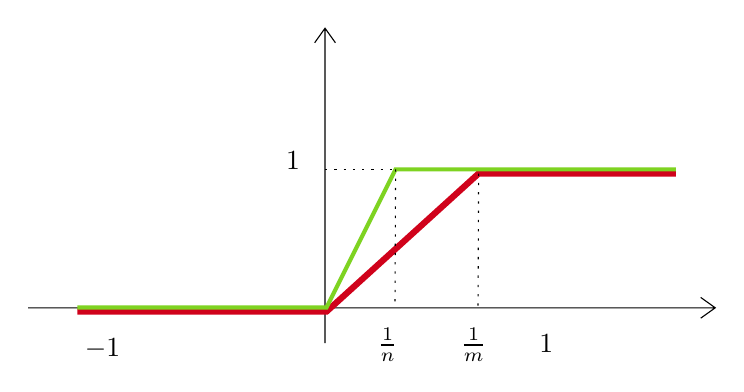
\begin{tikzpicture}[x=0.75pt,y=0.75pt,yscale=-1,xscale=1]
%uncomment if require: \path (0,197); %set diagram left start at 0, and has height of 197

%Shape: Axis 2D [id:dp7510112278083159] 
\draw  (141,140.7) -- (472,140.7)(284,6) -- (284,157.7) (465,135.7) -- (472,140.7) -- (465,145.7) (279,13) -- (284,6) -- (289,13)  ;
%Straight Lines [id:da35643943970375824] 
\draw [color={rgb, 255:red, 208; green, 2; blue, 27 } ,draw opacity=1 ][line width=2.25]    (453,76) -- (358,76) -- (284.7,142.53) -- (164.7,142.53) ;
%Straight Lines [id:da14888962981095388] 
\draw  [dash pattern={on 0.84pt off 2.51pt}]  (358,76) -- (357.7,142.53) ;
%Straight Lines [id:da7820546278212102] 
\draw [color={rgb, 255:red, 126; green, 211; blue, 33 } ,draw opacity=1 ][line width=1.5]    (453,74) -- (318,74) -- (284.7,140.53) -- (164.7,140.53) ;
%Straight Lines [id:da933791757163982] 
\draw  [dash pattern={on 0.84pt off 2.51pt}]  (318,74) -- (317.7,140.53) ;
%Straight Lines [id:da44978431803839936] 
\draw  [dash pattern={on 0.84pt off 2.51pt}]  (284,74) -- (318,74) ;

% Text Node
\draw (167,154.4) node [anchor=north west][inner sep=0.75pt]    {$-1$};
% Text Node
\draw (386,152.4) node [anchor=north west][inner sep=0.75pt]    {$1$};
% Text Node
\draw (348,149.4) node [anchor=north west][inner sep=0.75pt]    {$\frac{1}{m}$};
% Text Node
\draw (308,149.4) node [anchor=north west][inner sep=0.75pt]    {$\frac{1}{n}$};
% Text Node
\draw (264,64.4) node [anchor=north west][inner sep=0.75pt]    {$1$};


\end{tikzpicture}

\end{figure}
\FloatBarrier

Verifichiamo che è di Cauchy, supponiamo $\displaystyle m\leqslant n$
\begin{align*}
\Vert v_{n} -v_{m}\Vert ^{2}_{2} & =\int ^{1}_{-1}(v_{n}(x) -v_{m}(x))^{2} dx\\
 & =\cancel{\int ^{0}_{-1}} +\int ^{1/n}_{0} +\int ^{1/m}_{1/n} +\cancel{\int ^{1}_{1/m}}\\
 & =\int ^{1/n}_{0}(n-m)^{2} x^{2} dx+\int ^{1/m}_{1/n}(1-mx)^{2} dx\rightarrow 0
\end{align*}
È convergente a Heaviside, ma non è continua, quindi è \textit{fuori} dallo spazio delle funzioni continue.

Se inoltre consideriamo la norma solita delle funzioni continue notiamo che
\begin{equation*}
\Vert v_{n} -v_{m}\Vert _{C([ -1,1])} =\max_{x\in [ -1,1]}(v_{n}(x) -v_{m}(x)) =1-\frac{m}{n} \nrightarrow 0
\end{equation*}
per $n,m\rightarrow \infty $, infatti se scegliamo $\displaystyle n=2m$ il limite tenderebbe a $\displaystyle 1/2$.

In questo esempio:
\begin{itemize}
\item La successione è di Cauchy ma non converge
\item Lo spazio con $\Vert \cdotp \Vert _{2}$ non è completo
\item $\Vert \cdotp \Vert _{2}$ e $\Vert \cdotp \Vert _{C}$ non sono equivalenti
\end{itemize}
\begin{definition}
[Prodotto scalare] $(\cdotp,\cdotp) :X\times X\rightarrow \mathbb{R}$ tale che
\begin{itemize}
\item $(v,v) \geqslant 0$ e $(v,v) =0\Leftrightarrow v=0$
\item $(u,v) =(v,u),\forall u,v\in X$
\item $( \lambda _{1} u_{1} +\lambda _{2} u_{2},v) =\lambda _{1}(u_{1},v) +\lambda _{2}(u_{2},v),\forall \lambda _{1},\lambda _{2} \in \mathbb{R},\forall u_{1},u_{2},v\in X$
\end{itemize}
\end{definition}
\begin{definition}
Norma indotta dal prodotto scalare
\begin{equation*}
\Vert v\Vert =\sqrt{(v,v)}
\end{equation*}
\end{definition}
Esercizio. Verificare che il prodotto scalare è continuo rispetto alla norma indotta e che $\Vert \cdotp \Vert $ è una norma.
\begin{theorem}
Alcune proposizioni
\begin{enumerate}
\item Cauchy-Schwarz $| (u,v)| \leqslant \Vert u\Vert \cdotp \Vert v\Vert $
\item Identità del parallelogramma\footnote{la somma dei quadrati sulle diagonali è uguale alla somma dei quadrati su tutti i lati.} $\Vert u+v\Vert ^{2} +\Vert u-v\Vert ^{2} =2\Vert u\Vert ^{2} +2\Vert v\Vert ^{2}$, vale solo se la norma è indotta da un prodotto scalare
\end{enumerate}
\end{theorem}
\begin{definition}
Uno spazio vettoriale $X$, con prodotto scalare, che sia completo rispetto alla norma indotta dal prodotto scalare si dice \textbf{Spazio di Hilbert}.
\end{definition}
Esempi.

$\mathbb{R}^{n},L^{2}(\Omega)$ con la norma $(u,v)_{L^{2}(\Omega)} =\int _{\Omega } uvdx$

In uno spazio con prodotto scalare possiamo definire l'\textbf{ortogonalità}
\begin{equation*}
u\perp v\Leftrightarrow (u,v) =0
\end{equation*}
\section{Approssimazione di vettori}

Chiameremo $H$ un generico spazio di Hilbert. Considerando $\displaystyle H$ e $V\subset H$ sottospazio\footnote{$u,v\in V\Rightarrow \lambda u+\mu v\in V$.}, $x\in H$, vogliamo trovare il vettore di $V$ che meglio approssima $x$. Stiamo cercando $\overline{v} \in V$ tale che
\begin{equation*}
\Vert x-\overline{v}\Vert =\inf_{v\in V}\Vert x-v\Vert 
\end{equation*}



\begin{figure}[htpb]
	\centering

\tikzset{every picture/.style={line width=0.75pt}} %set default line width to 0.75pt        

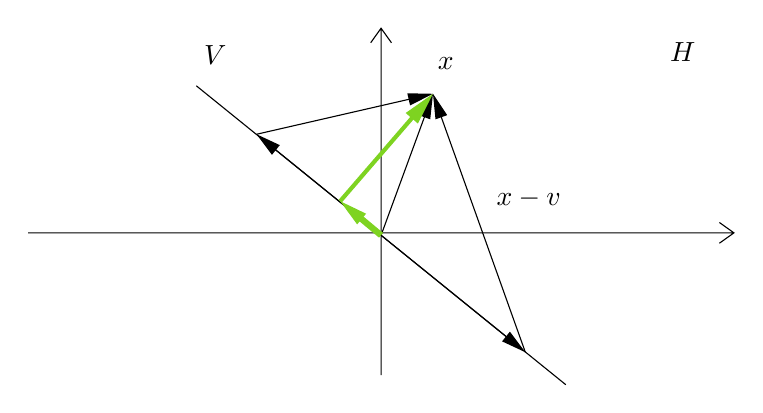
\begin{tikzpicture}[x=0.75pt,y=0.75pt,yscale=-1,xscale=1]
%uncomment if require: \path (0,198); %set diagram left start at 0, and has height of 198

%Straight Lines [id:da9073640143708681] 
\draw    (301,113.41) -- (242.55,66.01) ;
\draw [shift={(241,64.75)}, rotate = 399.03999999999996] [fill={rgb, 255:red, 0; green, 0; blue, 0 }  ][line width=0.08]  [draw opacity=0] (12,-3) -- (0,0) -- (12,3) -- cycle    ;
%Shape: Axis 2D [id:dp9737576348755399] 
\draw  (131,112.25) -- (471,112.25)(301,13.66) -- (301,180.75) (464,107.25) -- (471,112.25) -- (464,117.25) (296,20.66) -- (301,13.66) -- (306,20.66)  ;
%Straight Lines [id:da5543961945984461] 
\draw    (212,41.41) -- (390,185.41) ;
%Straight Lines [id:da7822239085129437] 
\draw    (301,113.41) -- (325.31,47.13) ;
\draw [shift={(326,45.25)}, rotate = 470.14] [fill={rgb, 255:red, 0; green, 0; blue, 0 }  ][line width=0.08]  [draw opacity=0] (12,-3) -- (0,0) -- (12,3) -- cycle    ;
%Straight Lines [id:da5022645915295285] 
\draw    (370.5,169.75) -- (326.67,47.13) ;
\draw [shift={(326,45.25)}, rotate = 430.33000000000004] [fill={rgb, 255:red, 0; green, 0; blue, 0 }  ][line width=0.08]  [draw opacity=0] (12,-3) -- (0,0) -- (12,3) -- cycle    ;
%Straight Lines [id:da8728054276938597] 
\draw    (241,64.75) -- (324.05,45.7) ;
\draw [shift={(326,45.25)}, rotate = 527.0799999999999] [fill={rgb, 255:red, 0; green, 0; blue, 0 }  ][line width=0.08]  [draw opacity=0] (12,-3) -- (0,0) -- (12,3) -- cycle    ;
%Straight Lines [id:da7420419315205793] 
\draw [color={rgb, 255:red, 126; green, 211; blue, 33 } ,draw opacity=1 ][line width=1.5]    (281.29,97) -- (323.38,48.28) ;
\draw [shift={(326,45.25)}, rotate = 490.83] [fill={rgb, 255:red, 126; green, 211; blue, 33 } ,fill opacity=1 ][line width=0.08]  [draw opacity=0] (15.6,-3.9) -- (0,0) -- (15.6,3.9) -- cycle    ;
%Straight Lines [id:da5034396510582315] 
\draw [color={rgb, 255:red, 126; green, 211; blue, 33 } ,draw opacity=1 ][line width=2.25]    (301,113.41) -- (285.9,100.84) ;
\draw [shift={(281.29,97)}, rotate = 399.77] [fill={rgb, 255:red, 126; green, 211; blue, 33 } ,fill opacity=1 ][line width=0.08]  [draw opacity=0] (13.44,-3.36) -- (0,0) -- (13.44,3.36) -- cycle    ;
%Straight Lines [id:da8018205092868931] 
\draw    (301,113.41) -- (368.95,168.49) ;
\draw [shift={(370.5,169.75)}, rotate = 219.03] [fill={rgb, 255:red, 0; green, 0; blue, 0 }  ][line width=0.08]  [draw opacity=0] (12,-3) -- (0,0) -- (12,3) -- cycle    ;

% Text Node
\draw (439,19.4) node [anchor=north west][inner sep=0.75pt]    {$H$};
% Text Node
\draw (214.5,20.9) node [anchor=north west][inner sep=0.75pt]    {$V$};
% Text Node
\draw (327.14,26.61) node [anchor=north west][inner sep=0.75pt]    {$x$};
% Text Node
\draw (355.43,90.04) node [anchor=north west][inner sep=0.75pt]    {$x-v$};


\end{tikzpicture}

\end{figure}
\FloatBarrier

$\displaystyle \overline{v}$ è la proiezione su $V$ di $x$, che indicheremo come $P_{V} x$, è l'elemento di minima distanza (\textit{se esiste}).
\begin{itemize}
\item in $\mathrm{dim} < +\infty $ esiste sempre (Gram-Schmidt).
\item in $\mathrm{dim} =\infty $ non è detto, servono ipotesi in più.
\end{itemize}

Nel caso di prima possiamo approssimare Heaviside con le approssimanti introdotte, ma non c'è \textit{la migliore}, questo ci dice che le funzioni continue non sono un sottospazio \textit{chiuso}.
\begin{theorem}
[delle Proiezioni] Sia $H$ di Hilbert, $V$ sottospazio vettoriale di $H$ \textbf{chiuso}\footnote{in senso topologico, deve contenere tutti i suoi punti di frontiera.}, $x\in H$. Allora $\exists !P_{V} x\in V$ tale che
\begin{equation*}
\Vert P_{V} x-x\Vert =\inf_{v\in V}\Vert v-x\Vert 
\end{equation*}
\textit{Lezione 2 (04/03/2021)}

\textbf{Inoltre:}
\begin{enumerate}
\item $\displaystyle x\in V\ \Leftrightarrow \ x=P_{V} x$
\item Definendo $\displaystyle Q_{V} x=x-P_{V} x\ \Rightarrow \ (Q_{V} x,v) =0\ \forall v\in V$

($\displaystyle \Longrightarrow \Vert x\Vert ^{2} =\Vert P_{V} x\Vert ^{2} +\Vert Q_{V} x\Vert ^{2}$ teorema di Pitagora)

cioè $\displaystyle Q_{V} x\in V^{\bot }$
\end{enumerate}
\end{theorem}
\begin{nb}
Se $\displaystyle \mathrm{dim} H\mathrm{=+\infty }$ non è detto che i sottospazi siano chiusi, a differenza di spazi a dimensione finita, però se
\begin{equation*}
\mathrm{dim} V< +\infty,\ V\subset H\ \ \Rightarrow \ V\ \text{chiuso}
\end{equation*}
e in ogni caso $\displaystyle V^{\bot }$è chiuso.
\end{nb}

\begin{dimostrazione}[Teorema delle Proiezioni]

\begin{itemize}
\item Esistenza\begin{equation*}
d=\inf_{v\in V}\Vert v-x\Vert,\ d\geqslant 0
\end{equation*}

ovvero, per definizione di $\displaystyle \inf$
\begin{enumerate}
\item $\displaystyle \Vert v-x\Vert \geqslant d,\ \forall v\in V$
\item $\displaystyle \forall \varepsilon \ \exists v_{\varepsilon } \in V$ tale che $\displaystyle \Vert v_{\varepsilon } -x\Vert \leqslant d+\varepsilon $ \ $ $
\end{enumerate}

uso la definizione per costruire una ``successione minimizzante''
\begin{equation}
(v_{n})_{n\in \mathbb{N}} \subset V:\ d\leqslant \Vert x-v_{n}\Vert \leqslant d+\frac{1}{n} \ \ \left( \varepsilon =\frac{1}{n},\ n\in \mathbb{N}\right)
\label{eq:teo-proiez-suc-min}
\end{equation}

voglio dimostrare che la successione converga, ma per farlo prima devo dimostrare che è una successione di Cauchy. Uso l'identità del parallelogramma riscritta nel seguente modo\begin{equation*}
\Vert a-b\Vert ^{2} =2\Vert a\Vert ^{2} +2\Vert b\Vert ^{2} -\Vert a+b\Vert ^{2}
\end{equation*}

con $\displaystyle a=v_{n} -x$, $\displaystyle b=v_{m} -x$, i termini dell'identità diventano:\begin{equation*}
\begin{array}{ l }
\Vert a-b\Vert ^{2} =\Vert v_{n} -v_{m}\Vert ^{2}\\
\Vert a+b\Vert ^{2} =\Vert v_{n} +v_{m} -2x\Vert ^{2} =4\bigg\Vert \underbrace{\frac{v_{n} +v_{m}}{2}}_{\in V} -x\bigg\Vert ^{2} \geqslant 4d^{2}
\end{array}
\end{equation*}

dove l'ultima disuguaglianza vale perché $\displaystyle \Vert v-x\Vert \geqslant d,\ \forall v\in V$ (definizione di $\displaystyle \inf$) e $\displaystyle \frac{v_{n} +v_{m}}{2} \in V$, essendo $\displaystyle V$ un sottospazio.

La norma di $\displaystyle a$ e di $\displaystyle b$ tenderà a $\displaystyle d$ per il teorema dei carabinieri e per \eqref{eq:teo-proiez-suc-min}. Sostituendo nell'identità\begin{align*}
0 & \leqslant \Vert v_{n} -v_{m}\Vert ^{2}\\
 & =2\Vert v_{n} -x\Vert ^{2} +2\Vert v_{m} -x\Vert ^{2} -4\left\Vert \frac{v_{n} +v_{m}}{2} -x\right\Vert ^{2}\\
 & \leqslant 2\Vert v_{n} -x\Vert ^{2} +2\Vert v_{m} -x\Vert ^{2} -4d^{2}\\
 & \xrightarrow[n,m\rightarrow \infty ]{} 2d^{2} +2d^{2} -4d^{2} =0
\end{align*}

Quindi la mia successione minimizzante è di Cauchy. Ma poiché $\displaystyle H$ è di Hilbert, ogni successione di Cauchy è convergente\begin{equation*}
v_{n}\xrightarrow{n\rightarrow \infty }\overline{v} \in H
\end{equation*}

e poiché $\displaystyle V$ è chiuso, $\displaystyle \overline{v} \in V$. Allora prendendo la definizione della mia successione \begin{equation*}
d\leqslant \Vert x-v_{n}\Vert \leqslant d+\frac{1}{n}
\end{equation*}

e facendone il limite per $\displaystyle n\rightarrow \infty $ ottengo\footnote{In questo passaggio è usata la continuità della norma (conseguenza banale della disuguaglianza triangolare)}\begin{equation*}
d\leqslant \Vert x-\overline{v}\Vert \leqslant d
\end{equation*}

Definisco la proiezione di $\displaystyle x$ su $\displaystyle V$: $\displaystyle \boxed{P_{V} x=\overline{v}}$
\item Unicità

Per assurdo\begin{equation*}
\overline{v},\overline{w} \in V,\ \ \Vert \overline{v} -x\Vert =\Vert \overline{w} -x\Vert =d
\end{equation*}

Usando l'identità del parallelogramma con $\displaystyle a=\overline{v} -x$, $\displaystyle b=\overline{w} -x$:\begin{equation*}
\Vert \overline{v} -\overline{w}\Vert ^{2} +\Vert \overline{v} +\overline{w} -2x\Vert ^{2} =4d^{2}
\end{equation*}

Sfruttando gli stessi passaggi dell'esistenza osservo che $\displaystyle \Vert \overline{v} +\overline{w} -2x\Vert ^{2} \geqslant 4d^{2}$. Allora perchè l'identità sia soddisfatta deve essere $\displaystyle \Vert \overline{v} -\overline{w}\Vert ^{2} \leqslant 0$ \begin{equation*}
\Rightarrow \ \ \Vert \overline{v} -\overline{w}\Vert ^{2} =0\ \ \Rightarrow \ \ \overline{v} =\overline{w}
\end{equation*}
\item Inoltre (punto 1)

conseguenza banale, se $\displaystyle x\in V$ \begin{equation*}
d=\inf_{v\in V}\Vert v-x\Vert =0
\end{equation*}

$\displaystyle \Rightarrow \ \Vert x-P_{V} x\Vert =0\ \Rightarrow \ x=P_{V} x$ 
\item Inoltre (punto 2)

$\displaystyle Q_{V} x=x-P_{V} x$

Osservo che $\displaystyle \forall v\in V,\ t\in \mathbb{R} \Longrightarrow (P_{V} x-tv) \in V$




\begin{figure}[H]
	\centering

\tikzset{every picture/.style={line width=0.75pt}} %set default line width to 0.75pt        

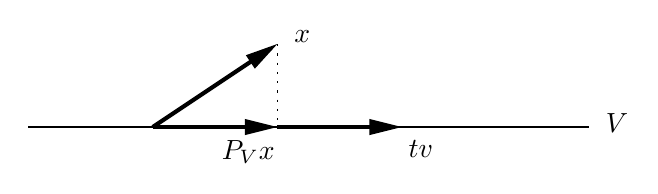
\begin{tikzpicture}[x=0.75pt,y=0.75pt,yscale=-1,xscale=1]
%uncomment if require: \path (0,98); %set diagram left start at 0, and has height of 98

%Straight Lines [id:da1966060419350555] 
\draw [color={rgb, 255:red, 0; green, 0; blue, 0 } ,draw opacity=1 ]   (90,60) -- (360,60) ;
%Straight Lines [id:da864357839898725] 
\draw [line width=1.5]    (150,60) -- (206,60) ;
\draw [shift={(210,60)}, rotate = 180] [fill={rgb, 255:red, 0; green, 0; blue, 0 }  ][line width=0.08]  [draw opacity=0] (15.6,-3.9) -- (0,0) -- (15.6,3.9) -- cycle    ;
%Straight Lines [id:da07495012975809501] 
\draw [line width=1.5]    (210,60) -- (266,60) ;
\draw [shift={(270,60)}, rotate = 180] [fill={rgb, 255:red, 0; green, 0; blue, 0 }  ][line width=0.08]  [draw opacity=0] (15.6,-3.9) -- (0,0) -- (15.6,3.9) -- cycle    ;
%Straight Lines [id:da21049925432833838] 
\draw [line width=1.5]    (150,60) -- (206.67,22.22) ;
\draw [shift={(210,20)}, rotate = 506.31] [fill={rgb, 255:red, 0; green, 0; blue, 0 }  ][line width=0.08]  [draw opacity=0] (15.6,-3.9) -- (0,0) -- (15.6,3.9) -- cycle    ;
%Straight Lines [id:da673978991154291] 
\draw  [dash pattern={on 0.84pt off 2.51pt}]  (210,20) -- (210,60) ;

% Text Node
\draw (182,65.4) node [anchor=north west][inner sep=0.75pt]    {$P_{V} x$};
% Text Node
\draw (272,65.4) node [anchor=north west][inner sep=0.75pt]    {$tv$};
% Text Node
\draw (217,12.4) node [anchor=north west][inner sep=0.75pt]    {$x$};
% Text Node
\draw (367,52.4) node [anchor=north west][inner sep=0.75pt]    {$V$};


\end{tikzpicture}

\end{figure}
\FloatBarrier
\begin{align*}
d^{2} & \leqslant \Vert -(P_{V} x-tv) +x\Vert ^{2} =\Vert Q_{V} x+tv\Vert ^{2}\\
 & =\Vert Q_{V} x\Vert ^{2} +2t(Q_{V} x,v) +t^{2}\Vert v\Vert ^{2}\\
 & =d^{2} +2t(Q_{V} x,v) +t^{2}\Vert v\Vert ^{2}\\
 & \\
 & \Rightarrow \ \ \Vert v\Vert ^{2} t^{2} +2(Q_{V} x,v) t\geqslant 0,\ \forall t\in \mathbb{R},\ \forall v\in V
\end{align*}

Per analogia con l'equazione di una parabola\begin{equation*}
at^{2} +bt+c\geqslant 0,\ \forall t\in \mathbb{R} \ \ \Rightarrow \ \ b^{2} -4ac\leqslant 0
\end{equation*}

Con $\displaystyle a=\Vert v\Vert ^{2},\ b=2(Q_{V} x,v)$

Ma se $\displaystyle c=0\ \Rightarrow \ b\ =0$, da cui la tesi.
\item Teorema di Pitagora\begin{equation*}
\Vert x\Vert ^{2} =\Vert P_{V} x+Q_{V} x\Vert ^{2} =\Vert P_{V} x\Vert ^{2} +2(P_{V} x,Q_{V} x) +\Vert Q_{V} x\Vert ^{2}
\end{equation*}

dove il prodotto scalare è nullo per l'ortogonalità appena dimostrata.
\end{itemize}
\end{dimostrazione}
\section{Operatori lineari}
\begin{definition}
[Operatore lineare] $\displaystyle H_{1},H_{2}$ di Hilbert, $\displaystyle L:H_{1}\rightarrow H_{2}$ è lineare se $\displaystyle L(\lambda u+\mu v) =\lambda L(u) +\mu L(v),\ u,v\in H_{1},\ \lambda,\mu \in \mathbb{R}$
\end{definition}
\begin{nb}
In spazi infinito dimensionali $\displaystyle L$ lineare $\displaystyle \nRightarrow $$\displaystyle L$ continuo, per cui lo richiederò come ipotesi.
\end{nb}
\begin{definition}
[Operatore limitato] $\displaystyle L$ (lineare) si dice limitato se $\displaystyle \exists c\geqslant 0$ t.c. $\displaystyle \Vert Lv\Vert _{H_{2}} \leqslant c\Vert v\Vert _{H_{1}} \forall v\in H_{1}$
\end{definition}
Osserviamo che 
\begin{equation*}
c\geqslant \frac{\Vert Lv\Vert _{H_{2}}}{\Vert v\Vert _{H_{1}}} =\left\Vert \frac{1}{\Vert v\Vert _{1}} Lv\right\Vert _{2} =\left\Vert L\left(\frac{v}{\Vert v\Vert _{1}}\right)\right\Vert _{2}
\end{equation*}
dove $\displaystyle \frac{v}{\Vert v\Vert _{1}}$ ha norma 1, quindi $\displaystyle L$ è limitato se e solo se
\begin{equation*}
\sup _{\Vert x\Vert =1}\Vert Lx\Vert _{2} =k< +\infty 
\end{equation*}
$\displaystyle k$ è la miglior costante di limitatezza e prende il nome di \textbf{norma operatoriale}.
\begin{theorem}
Sia $\displaystyle L$ un operatore lineare. Allora
\begin{equation}
L\ \text{continuo} \ \ \Leftrightarrow \ \ L\ \text{limitato}
\label{eq:continuo-limitato}
\end{equation}
\end{theorem}
\begin{dimostrazione}[di $\displaystyle (\Leftarrow)$]
$\displaystyle L$ limitato $\displaystyle \Rightarrow \Vert Lx\Vert _{2} \leqslant C\Vert x\Vert _{1},\ x=v-v_{0}$
\begin{equation*}
0\leqslant \Vert Lv-Lv_{0}\Vert _{2} =\Vert L(v-v_{0})\Vert _{2} \leqslant c\Vert v-v_{0}\Vert _{1}
\end{equation*}
(ho dimostrato così che $\displaystyle L$ è Lipschitz-continua).
\end{dimostrazione}
\begin{definition}
$\displaystyle \mathcal{L}(H_{1},H_{2}) =\{L:H_{1}\rightarrow H_{2}$ lineari e continui$\displaystyle \}$
\begin{equation*}
\Vert L\Vert _{\mathcal{L}(H_{1},H_{2})} =\text{(miglior costante di limitatezza)} =\sup _{\Vert x\Vert _{1} =1}\Vert Lx\Vert _{2}
\end{equation*}
\end{definition}
\begin{theorem}
$\displaystyle \mathcal{L}(H_{1},H_{2})$ è di Banach.
\end{theorem}
\textbf{Esempio importante (immersione)}

$\displaystyle H_{1} \subset H_{2}$ sottospazio (eventualmente con norme non equivalenti)

$\displaystyle L:\ \underbrace{x}_{\in H_{1}} \ \rightarrow \underbrace{x}_{\in H_{2}}$, $\displaystyle x$ è lo stesso elemento di due spazi con norme differenti. 

Data un'immersione $\displaystyle L(x) =x$, quando è continua? Per \eqref{eq:continuo-limitato}, è continua $\displaystyle \Leftrightarrow $ è limitata, ovvero $\displaystyle \Vert x\Vert _{H_{2}} \leqslant c\Vert x\Vert _{H_{1}} \forall x\in H_{1}$. In questo caso l'immersione prende il nome di \textbf{immersione continua.}

Un esempio pratico è lo spazio $\displaystyle C([ 0,1]) \subset L^{2}(0,1)$, nel primo usiamo come norma il max, nel secondo la norma $\displaystyle \left(\int | \cdot | ^{2}\right)^{1/2}$, quindi possiamo misurare gli elementi di $\displaystyle C([ 0,1])$ con entrambe le norme. La notazione per indicare l'immersione è
\begin{equation*}
\ C([ 0,1]) \hookrightarrow L^{2}(0,1)
\end{equation*}
Dimostriamo ora la limitatezza dell'immersione (e quindi la continuità)
\begin{equation*}
\Vert u\Vert _{L^{2}(0,1)} =\sqrt{\int ^{1}_{0} u^{2}(x) dx} \leqslant \sqrt{\left(\max_{[ 0,1]} u^{2}\right) \cdot \int ^{1}_{0} 1dx} =\max_{[ 0,1]}| u| 
\end{equation*}
\begin{definition}
[Funzionale] Sia $\displaystyle H_{1} =H$ spazio di Hilbert, $\displaystyle H_{2} =\mathbb{R}$, $\displaystyle L:H\rightarrow \mathbb{R}$ è detto funzionale.
\end{definition}
\begin{definition}
[Spazio duale] È detto spazio duale di $\displaystyle H$, denotato con $\displaystyle H^{*}$
\begin{equation*}
H^{*} =\mathcal{L}(H,\mathbb{R}) =\left\{L:H\rightarrow \mathbb{R} \ \text{funzionali lineari e continui}\right\}
\end{equation*}
con norma
\begin{equation*}
\Vert L\Vert _{H^{*}} =\Vert L\Vert _{*} =\sup _{\Vert v\Vert =1}| Lv| 
\end{equation*}
\end{definition}
\textbf{Esempio 1.}

Sia $\displaystyle H=L^{2}(0,1),\ L:L^{2}(0,1)\rightarrow \mathbb{R},\ Lv=\int ^{1/2}_{0} v(x) dx$. Verifico che $\displaystyle L\in H^{*}$, ovvero che sia lineare, ben definito e continuo (limitato). L'operatore è chiaramente lineare perchè definito con integrale, è ben definito e continuo perché
\begin{equation*}
| Lv| =\left| \int ^{1/2}_{0} v(x) dx\right| \leqslant \int ^{1/2}_{0}| v(x)| dx\leqslant \int ^{1}_{0}| v(x)| dx
\end{equation*}
Utilizzando la disuguaglianza di Holder posso maggiorare l'ultimo termine
\begin{equation*}
\leqslant \left(\int ^{1}_{0} 1^{2}\right)^{1/2}\left(\int ^{1}_{0} v^{2}\right)^{1/2} =\Vert v\Vert _{L^{2}(0,1)}
\end{equation*}
Quindi $\displaystyle L\in H^{*},\ \Vert L\Vert _{*} \leqslant 1$.



\textbf{Esempio 2.}

Sia $\displaystyle H$ spazio di Hilbert, $\displaystyle u\in H$ fissato. Definisco $\displaystyle L_{u} v=Lv=(u,v)$

$\displaystyle L:v\rightarrow (u,v)$ è lineare (per linearità del prodotto scalare), inoltre
\begin{equation*}
| Lv| =| (u,v)| \leqslant \Vert u\Vert \Vert v\Vert 
\end{equation*}
per Cauchy-Schwartz. Quindi $\displaystyle L$ è lineare e continuo (limitato) allora $\displaystyle L\in H^{*}$, e $\displaystyle \Vert L\Vert _{*} \leqslant \Vert u\Vert $. Ma possiamo anche osservare che 
\begin{equation*}
\Vert L\Vert _{*} =\sup _{\Vert v\Vert =1}| Lv| \geqslant \left| L\left(\frac{u}{\Vert u\Vert }\right)\right| =\frac{1}{\Vert u\Vert }(u,u) =\frac{1}{\Vert u\Vert }\Vert u\Vert ^{2} =\Vert u\Vert 
\end{equation*}
Quindi $\displaystyle \Vert L\Vert _{*} \leqslant \Vert u\Vert $, $\displaystyle \Vert L\Vert _{*} \geqslant \Vert u\Vert $ allora $\displaystyle \Vert L\Vert _{*} =\Vert u\Vert $. Il teorema che vedremo ora ci confermerà che questo non è solo un esempio, ma l'unico caso possibile.

\textit{Lezione 3 (18/03/2021)}
\begin{theorem}
[di rappresentazione di Riesz] Sia $H$ uno spazio di Hilbert, allora $\forall L\in H^{*}$ esiste un unico vettore $u\in H$ tale che
\begin{equation*}
Lv=(u,v),\ \ \forall v\in H
\end{equation*}
Inoltre
\begin{equation*}
\Vert u\Vert =\Vert L\Vert _{*}
\end{equation*}
\end{theorem}
\begin{oss}
Il teorema di rappresentazione di Riesz è in realtà un teorema di buona posizione, dimostra infatti che
\begin{equation*}
\langle\langle \ \text{dato} \ L\in H^{*} \ \text{trovare} \ u\in H\ \text{tale che} \ Lv=(u,v),\ \forall v\in H\ \rangle\rangle 
\end{equation*}
è ben posto: garantisce l'esistenza e unicità di $\displaystyle u$, inoltre dati $\displaystyle L_{1},L_{2}$ e le soluzioni $\displaystyle u_{1},u_{2}$
\begin{gather*}
(u_{1},v) =L_{1} v\\
(u_{2},v) =L_{2} v
\end{gather*}
Per il principio di sovrapposizione (il problema è lineare):
\begin{equation*}
(u_{1} -u_{2},v) =(L_{1} -L_{2}) v\ \ \Rightarrow \ \ \Vert u_{1} -u_{2}\Vert =\Vert L_{1} -L_{2}\Vert _{*}
\end{equation*}
il problema è stabile (dipende con continuità dai dati).
\end{oss}
\begin{dimostrazione}
L'ultima affermazione in realtà l'abbiamo già dimostrata nell'esempio 2.
\textit{Esistenza.}
\begin{itemize}
\item Caso $1$: $\mathrm{Ker} L=H$

ovvero $Lv=0,\forall v$, in tal caso scelgo $u=0$.
\item Caso $2$: $\mathrm{Ker} L\varsubsetneqq H$

ovvero esiste un vettore $z_{0} \in H$ che non appartiene al nucleo $Lz_{0} \neq 0$. L'idea geometrica è molto semplice, vogliamo usare il teorema delle proiezioni e scegliere come $u$ il vettore ortogonale al nucleo, normalizzato




\begin{figure}[H]
	\centering

\tikzset{every picture/.style={line width=0.75pt}} %set default line width to 0.75pt        

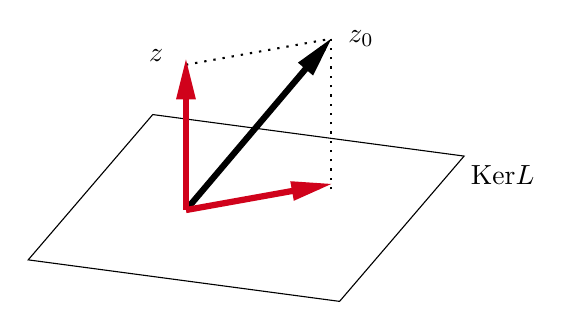
\begin{tikzpicture}[x=0.75pt,y=0.75pt,yscale=-1,xscale=1]
%uncomment if require: \path (0,152); %set diagram left start at 0, and has height of 152

%Straight Lines [id:da7968494763005547] 
\draw [color={rgb, 255:red, 0; green, 0; blue, 0 } ,draw opacity=1 ][line width=0.75]  [dash pattern={on 0.84pt off 2.51pt}]  (256,26) -- (326,13.44) ;
%Shape: Polygon [id:ds47696393353033595] 
\draw   (330,140) -- (180,120) -- (240,50) -- (390,70) -- cycle ;
%Straight Lines [id:da04367598648625459] 
\draw [line width=2.25]    (256,96) -- (322.12,18.01) ;
\draw [shift={(326,13.44)}, rotate = 490.29] [fill={rgb, 255:red, 0; green, 0; blue, 0 }  ][line width=0.08]  [draw opacity=0] (19.2,-4.8) -- (0,0) -- (19.2,4.8) -- cycle    ;
%Straight Lines [id:da8880773272488094] 
\draw [color={rgb, 255:red, 208; green, 2; blue, 27 } ,draw opacity=1 ][line width=2.25]    (256,96) -- (320.09,84.5) ;
\draw [shift={(326,83.44)}, rotate = 529.8299999999999] [fill={rgb, 255:red, 208; green, 2; blue, 27 } ,fill opacity=1 ][line width=0.08]  [draw opacity=0] (19.2,-4.8) -- (0,0) -- (19.2,4.8) -- cycle    ;
%Straight Lines [id:da3687846316598724] 
\draw [color={rgb, 255:red, 208; green, 2; blue, 27 } ,draw opacity=1 ][line width=2.25]    (256,96) -- (256,29.44) ;
\draw [shift={(256,23.44)}, rotate = 450] [fill={rgb, 255:red, 208; green, 2; blue, 27 } ,fill opacity=1 ][line width=0.08]  [draw opacity=0] (19.2,-4.8) -- (0,0) -- (19.2,4.8) -- cycle    ;
%Straight Lines [id:da07890995266380374] 
\draw [color={rgb, 255:red, 0; green, 0; blue, 0 } ,draw opacity=1 ][line width=0.75]  [dash pattern={on 0.84pt off 2.51pt}]  (326,86) -- (326,13.44) ;

% Text Node
\draw (392,73.4) node [anchor=north west][inner sep=0.75pt]    {$\mathrm{Ker} L$};
% Text Node
\draw (333,8.4) node [anchor=north west][inner sep=0.75pt]    {$z_{0}$};
% Text Node
\draw (237,17.4) node [anchor=north west][inner sep=0.75pt]    {$z$};


\end{tikzpicture}

\end{figure}
\FloatBarrier


Scegliamo quindi $H,V=\mathrm{Ker} L,x=z_{0}$, dobiamo verificare che $V$ è un sottospazio chiuso topologicamente per applicare le proiezioni.
\begin{itemize}
\item È un sottospazio, vogliamo dimostrare che\begin{equation*}
v_{1},v_{2} \in \mathrm{Ker} L\ \ \Rightarrow \ \ \lambda _{1} v_{1} +\lambda _{2} v_{2} \in \mathrm{Ker} L
\end{equation*}

ovvero che\begin{equation*}
Lv_{1} =Lv_{2} =0\ \ \Rightarrow \ \ L( \lambda _{1} v_{1} +\lambda _{2} v_{2}) =0
\end{equation*}

ma per \textbf{linearità} di $L$ è soddisfatta\begin{equation*}
L( \lambda _{1} v_{1} +\lambda _{2} v_{2}) =\lambda _{1} Lv_{1} +\lambda _{2} Lv_{2} =0
\end{equation*}
\item Che sia chiuso è leggermente più delicato, osserviamo intanto che per definizione\begin{equation*}
\text{chiuso} \ \ \Leftrightarrow \ \ \left\{\begin{array}{ l }
(v_{n})_{n} \subset \mathrm{Ker} L\\
v_{n}\rightarrow \overline{v} \in H
\end{array} \Rightarrow \overline{v} \in \mathrm{Ker} L\right\}
\end{equation*}nel nostro caso\begin{equation*}
(v_{n})_{n} \subset \mathrm{Ker} L\ \ \Leftrightarrow \ \ Lv_{n} =0
\end{equation*}è vero che $L\overline{v} =0$? Sì grazie alla \textbf{continuità}.
\end{itemize}

Allora possiamo applicare il teorema delle proiezioni\begin{equation*}
z=\frac{z_{0} -P_{\mathrm{Ker} L} z_{0}}{\Vert z_{0} -P_{\mathrm{Ker} L} z_{0}\Vert }
\end{equation*}con questa scelta, si ha $z\in (\mathrm{Ker} L)^{\perp }$ e $\Vert z\Vert =1$. Abbiamo\begin{equation*}
v\in H\ \ \ \ z\in (\mathrm{Ker} L)^{\perp }
\end{equation*}costruiamo $w\in \mathrm{Ker} L$ che sia combinazione di quei due\begin{equation*}
w=v-\frac{Lv}{Lz} z\ \ \Rightarrow \ \ Lw=L\left( v-\frac{Lv}{Lz} z\right) =Lv-\frac{Lv}{Lz} Lz=0
\end{equation*}Notiamo che dato che $w\in \mathrm{Ker} L,z\in (\mathrm{Ker} L)^{\perp }$ allora $(w,z) =0$, pertanto\begin{equation*}
0=(w,z) =\left( v-\frac{Lv}{Lz} z,z\right) =(v,z) -\frac{Lv}{Lz}\underbrace{(z,z)}_{\Vert z\Vert ^{2} =1}
\end{equation*}infine\begin{equation*}
Lv=Lz(z,v) =(\underbrace{(Lz) z}_{u},v),\ \ \forall v\in H
\end{equation*}
\end{itemize}

\textit{Unicità.}

Supponiamo che questo vettore $u$ non sia unico, cioè che ne esistano due $u_{1},u_{2} \in H$ tali che
\begin{gather*}
(u_{1},v) =Lv,\ \forall v\in H\\
(u_{2},v) =Lv,\ \forall v\in H
\end{gather*}
sottraiamo membro a membro
\begin{equation*}
(u_{1} -u_{2},v) =0,\ \ \forall v\in H
\end{equation*}
questo implica che $u_{1} -u_{2} =0$.\footnote{Questa ultima implicazione non può essere fatta con troppa leggerezza, infatti siamo in uno spazio astratto e l'unica cosa che abbiamo sono le definizioni e i teoremi. Il fatto che quella cosa valga per ogni $v$, significa in particolare che vale anche per $v=u_{1} -u_{2}$, degli altri infiniti $v$ non ci interessa. Con tale scelta
\begin{equation*}
0=( u_{1} -u_{2},u_{1} -u_{2}) =\Vert u_{1} -u_{2}\Vert ^{2}
\end{equation*}
Per la proprietà di annullamento della norma
\begin{equation*}
\Vert u_{1} -u_{2}\Vert ^{2} =0\ \ \Leftrightarrow \ \ u_{1} -u_{2} =0
\end{equation*}
Alternativamente per la proprietà di annullamento del prodotto scalare
\begin{equation*}
( u_{1} -u_{2},u_{1} -u_{2}) =0\ \ \Leftrightarrow \ \ u_{1} -u_{2} =0
\end{equation*}}
\end{dimostrazione}
\begin{definition}
La scrittura $a:H\times H\rightarrow \mathbb{R}$ denota una \textbf{forma bilineare} se
\begin{itemize}
\item fissato $u$,\begin{equation*}
v\mapsto a(u,v) \ \ \text{è lineare in} \ v
\end{equation*}
\item fissato $v$,\begin{equation*}
u\mapsto a(u,v) \ \ \text{è lineare in} \ u
\end{equation*}
\end{itemize}
\end{definition}
\begin{definition}
Inoltre
\begin{itemize}
\item $a$ si dice \textbf{simmetrica} se

\begin{equation*}
a(u,v) =a(v,u),\ \ \forall v,u\in H
\end{equation*}

in generale non lo sarà, ma un esempio ne è il prodotto scalare.
\item $a$ si dice \textbf{continua} (\textbf{limitata}) se

\begin{equation*}
\exists M:\ \ | a(u,v)| \leqslant M\Vert u\Vert \Vert v\Vert,\ \ \forall v,u
\end{equation*}
\item $a$ si dice \textbf{coerciva/coercitiva} se

\begin{equation*}
\exists \alpha  >0\ \text{(costante di coercività)} :\ \ a(u,u) \geqslant \alpha \Vert u\Vert ^{2}
\end{equation*}
\end{itemize}
\end{definition}
Il prodotto scalare è un caso particolare di forma bilineare simmetrica $a(u,v) =(u,v)$, vediamo quanto valgono le costanti $M$ e $\alpha $. Per Cauchy-Schwarz
\begin{equation*}
| (u,v)| \leqslant \Vert u\Vert \Vert v\Vert \ \ \Rightarrow \ \ M=1
\end{equation*}
Per definizione di norma indotta dal prodotto scalare
\begin{equation*}
(u,u) =\Vert u\Vert ^{2} \ \ \Rightarrow \ \ \alpha =1
\end{equation*}
Il teorema di Lax-Milgram generalizza queste nozioni e ci permette di risolvere\footnote{esistenza, unicità e dipendenza continua.} il seguente problema.\footnote{da qui nascono i metodi di Galerkin.}
\begin{definition}
[Problema Variazionale Astratto, PVA] Dato $L\in H^{*}$ trovare $u\in H$ tale che
\begin{equation*}
a(u,v) =Lv,\ \ \forall v\in H
\end{equation*}
dove $a$ è una forma bilineare.
\end{definition}
Nel caso di prodotto scalare $a(u,v) =(u,v)$, (PVA) diventa $(u,v) =Lv$ che è ben posto per il teorema di Riesz.
\begin{theorem}
[di Lax-Milgram] Siano
\begin{itemize}
\item $H$ spazio di Hilbert
\item $a$ forma bilineare continua e coerciva
\item $L\in H^{*}$
\end{itemize}

Allora $\exists !\ \overline{u} \in H$ soluzione di (PVA). Inoltre (\textbf{stima di stabilità})
\begin{equation*}
\Vert \overline{u}\Vert \leqslant \frac{1}{\alpha }\Vert L\Vert _{*}
\end{equation*}
dove $\alpha $ è la costante di coercività, ci interessa che sia più grande possibile.
\end{theorem}
\begin{oss}
La stabilità è utile considerando due dati vicini e due soluzioni vicine. Prendiamo ad esempio due soluzioni $u_{1},u_{2}$ soluzioni del (PVA) coi dati $L_{1} v,L_{2} v$
\begin{gather*}
a(u_{1},v) =L_{1} v,\ \ \forall v\in H\\
a(u_{2},v) =L_{2} v,\ \ \forall v\in H
\end{gather*}
Facciamo la differenza e usiamo la linearità
\begin{equation*}
a(u_{1} -u_{2},v) =(L_{1} -L_{2}) v
\end{equation*}
La stima di stabilità ci dice che
\begin{equation*}
\Vert u_{1} -u_{2}\Vert \leqslant \frac{1}{\alpha }\Vert L_{1} -L_{2}\Vert _{*}
\end{equation*}
Ovvero a \textit{dati vicini} sono associate \textit{soluzioni vicine}, a patto che $\alpha $ sia sufficientemente grande.
\end{oss}
\begin{dimostrazione}
Proponiamo un'overview dei passi della dimostrazione
\begin{enumerate}
\item[(0)] Riscrittura del problema in termini di $A$
\item[(1)] $A$ è lineare
\item[(2)] $A$ è continuo (ovvero limitato)
\item[(3)] $A$ è iniettivo (ovvero $\mathrm{Ker} A=\{0\}$)
\item[(3.5)] l'immagine $R(A)$ è un sottospazio chiuso, cosa \textbf{non} vera in generale
\item[(4)] $A$ è suriettivo (ovvero $R(A) =H$)
\end{enumerate}
Procediamo quindi con la dimostrazione
\begin{itemize}
\item[(0)]

Notiamo che la $v$ è una sorta di \textit{funzione test}, infatti vogliamo ottenere una cosa che vale per infiniti $v$. Al secondo membro del (PVA), per ipotesi $L\in H^{*}$, allora per Riesz $\exists !\ z\in H$ tale che $Lv=(z,v),\forall v$ e inoltre $\Vert z\Vert =\Vert L\Vert _{*}$. Vogliamo applicarlo anche al primo membro. Per definizione di forma bilineare, $\forall u$ fissato, l'applicazione $v\mapsto a(u,v)$ è lineare e continua in $v$, infatti\footnote{usando la continuità di $a$.}
\begin{equation*}
\text{continua} \ \ \Leftrightarrow \ \ | a(u,v)| \leqslant \underbrace{M\Vert u\Vert }_{C}\Vert v\Vert \leqslant C\Vert v\Vert 
\end{equation*}
allora per Riesz per ogni $u$ fissato $\exists !\ h=A(u) \in H$ tale che
\begin{equation*}
a(u,v) =(h,v),\ \ \forall v
\end{equation*}
cioè ho definito un'applicazione $A:H\rightarrow H$ tale che
\begin{equation*}
\boxed{a(u,v) =(A(u),v),\ \forall v\in H}
\end{equation*}
noi vogliamo dimostrare su $A$, ma abbiamo proprietà su $a$, questa relazione è la \textbf{chiave!}

Avendo così usato due volte il teorema di Riesz per passare da due operatori lineari a due prodotti scalari, il (PVA) diventa
\begin{equation*}
(A(u),v) =(z,v) \ \ \forall v\in H
\end{equation*}
Sottraiamo membro a membro e deduciamo, con la proprietà di annullamento del prodotto scalare
\begin{equation*}
(A(u) -z,v) =0,\ \forall v\in H\ \ \Rightarrow \ \ \boxed{A(u) =z}
\end{equation*}
risolvere (PVA) quindi \textit{è come} trovare l'operatore \textit{inverso} di $A$.



\item[(1)]

Dobbiamo sempre lavorare con il prodotto scalare di $A$ per qualcosa, in modo da usare la chiave trovata al passo precedente
\begin{equation*}
( A( \lambda u_{1} +\mu u_{2}),v) =a( \lambda u_{1} +\mu u_{2},v) =(*)
\end{equation*}
da qui è tutto automatico
\begin{align*}
(*) & =\lambda a(u_{1},v) +\mu a(u_{2},v)\\
 & =\lambda (A(u_{1}),v) +\mu (A(u_{2}),v)\\
 & =(\lambda A(u_{1}) +\mu A(u_{2}),v) \ \ \forall v\in H
\end{align*}
cioè $A( \lambda u_{1} +\mu u_{2}) =\lambda A(u_{1}) +\mu A(u_{2})$.

D'ora in poi useremo la \textbf{notazione}
\begin{equation*}
A(u) =Au
\end{equation*}


\item[(2)]

Notiamo che
\begin{equation*}
\Vert Au\Vert ^{2} =(Au,Au) =a(u,Au) \leqslant | a(u,Au)| \leqslant M\Vert u\Vert \Vert Au\Vert 
\end{equation*}
allora
\begin{equation*}
\Vert Au\Vert \leqslant M\Vert u\Vert 
\end{equation*}
Se $\Vert Au\Vert $ fosse stato $0$ non avrei avuto nulla dimostrare, per cui ho potuto semplificare.



\item[(3)]

È l'unico in cui non possiamo mettere il pilota automatico. Qui troveremo anche la stima di stabilità. Per farlo dobbiamo partire dalla coercività
\begin{equation*}
\alpha \Vert u\Vert ^{2} \leqslant a(u,u) =(Au,u) \leqslant | (Au,u)| \underbrace{\leqslant }_{\text{C.S.}}\Vert Au\Vert \Vert u\Vert \ \ \alpha  >0
\end{equation*}
Possiamo dividere per $u$ perché se fosse $0$ sarebbe soddisfatta già, otteniamo la stima di stabilità
\begin{equation*}
\Vert u\Vert \leqslant \frac{1}{\alpha }\Vert Au\Vert 
\end{equation*}
Nel nuovo (PVA) $Au=z$ e ricordiamo che $z$ era il vettore che rappresentava $L$ (come visto al passo 0)
\begin{equation*}
\Vert u\Vert \leqslant \frac{1}{\alpha }\Vert Au\Vert =\frac{1}{\alpha }\Vert z\Vert =\frac{1}{\alpha }\Vert L\Vert _{*}
\end{equation*}
Se $u\in \mathrm{Ker} A$ allora $Au=0$, usando la stima $\Vert u\Vert \leqslant 0$, allora $u=0$. Quindi $\mathrm{Ker} A=\{0\}$, ovvero $A$ è iniettivo.



\item[(3.5)]

L'immagine è un sottospazio, analogo a come visto prima.

Dimostriamo che è chiuso, ovvero che considerando ogni successione conenuta nell'immagine $(y_{n})_{n} \subset R(A)$ che tende a un certo valore $y_{n}\rightarrow \overline{y}$ allora quel valore sta nell'immagine $\overline{y} \in R(A)$\footnote{ricordiamo che la definizione è \textit{interessante} se consideriamo i punti del bordo in particolare.}.

Questi valori dell'immagine sono associati agli elementi del dominio $y_{n} =Au_{n}$, ci piacerebbe dire che $\overline{y} =A\overline{u}$, con $\overline{u} =\lim u_{n}$, \textbf{ma questo limite non è detto che esista! In un sacco di situazioni concrete salta!}

Ci rivolgiamo nuovamente alla completezza dello spazio, dimostrando che è una successione di Cauchy, usando la stima di stabilità del passo 3
\begin{equation*}
0\leqslant \Vert u_{n} -u_{m}\Vert \underbrace{\leqslant }_{(3)}\frac{1}{\alpha }\Vert A(u_{n} -u_{m})\Vert \underbrace{\leqslant }_{\text{lin.}}\frac{1}{\alpha }\Vert Au_{n} -Au_{m}\Vert =\frac{1}{\alpha }\Vert y_{n} -y_{m}\Vert 
\end{equation*}
la successione $y_{n}$ è convergente, quindi anche di Cauchy, allora l'ultimo termine tende a $0$, in particolare quindi anche $u_{n}$ è di Cauchy, ma essendo $H$ completo è anche convergente a un certo $\overline{u} \in H$.

Usanndo la continuità di $A$, $Au_{n}\rightarrow A\overline{u}$, quindi $\overline{y} =A\overline{u} \in R(A)$.



\item[(4)]

Supponiamo per assurdo che
\begin{equation*}
R(A) \varsubsetneqq H
\end{equation*}
cioè esiste $z_{0} \in H$, $z_{0} \notin R(A)$. Per il teorema delle proiezioni\footnote{che possiamo applicare avendo dimostrato che l'immagine $R(A)$ è un sottospazio chiuso al passo 3.5}
\begin{equation*}
z=\frac{z_{0} -P_{R(A)} z_{0}}{\Vert z_{0} -P_{R(A)} z_{0}\Vert } \ \ \Rightarrow \ \ z\in (R(A))^{\perp },\ \Vert z\Vert =1
\end{equation*}
A questo punto notiamo che
\begin{equation*}
z\in (R(A))^{\perp },\ \ Az\in R(A) \ \ \Rightarrow \ \ (z,Az) =0
\end{equation*}
Andando alla definizione di $A$
\begin{equation*}
(z,Az) =a(z,z) \geqslant \alpha \Vert z\Vert ^{2} =\alpha  >0
\end{equation*}
Ma ciò è assurdo, è quindi negata la supposizione iniziale e $R(A) =H$.
\end{itemize}
\end{dimostrazione}


\end{document}
